\documentclass[binding=0.6cm,oneside,noexaminfo]{sapthesis}
% Sapienza "Laurea Magistrale" thesis class. sapthesis.cls, the Sapienza logo
% (sapienzalogo.pdf) and sapthesis.bst are vendored next to this file, so the
% document compiles locally with no system-wide install and no biber.
\usepackage[utf8]{inputenc}
\usepackage[T1]{fontenc}
\usepackage{setspace}
\onehalfspacing

% "demo" makes \includegraphics draw a placeholder box instead of loading a
% file -- so this compiles with NO image files. Remove "demo" once you add the
% real images (and set \graphicspath to their folder).
\usepackage{graphicx}
\usepackage{float}        % [H] = pin a float exactly where it is placed
\usepackage{booktabs}     % \toprule \midrule \bottomrule
\usepackage{multirow}     % \multirow in results tables
\usepackage{array}
\usepackage{tabularx}     % stretching table + the custom "L" column below
\usepackage{enumitem}
\usepackage[hidelinks]{hyperref}
\usepackage[T1]{fontenc}
\usepackage[utf8]{inputenc}
\usepackage{lmodern}
\usepackage{microtype}
\usepackage{amsmath,amssymb,amsthm}
\usepackage{mathtools}
\usepackage{xcolor}
\usepackage{booktabs}
% geometry intentionally NOT loaded: sapthesis controls the page layout.
\usepackage{cleveref}
\usepackage{algorithm}
\usepackage{algpseudocode}
\usepackage{enumitem}
\usepackage{mdframed}
\usepackage{cleveref}     % \cref \Cref
\newtheorem{claim}{Claim}
\newtheorem{definition}{Definition}

%% ── Pretty shell-command listings ───────────────────────────────────────────
\usepackage{listings}
\definecolor{lstbg}{gray}{0.97}
\definecolor{lstframe}{gray}{0.78}
\definecolor{lstcomment}{rgb}{0.16,0.50,0.20}
\definecolor{lstkw}{rgb}{0.10,0.25,0.65}
\definecolor{lstnum}{gray}{0.55}
\lstdefinestyle{shell}{%
  basicstyle=\ttfamily\footnotesize,
  backgroundcolor=\color{lstbg},
  frame=single,
  rulecolor=\color{lstframe},
  framesep=7pt,
  xleftmargin=20pt,
  xrightmargin=6pt,
  numbers=left,
  numberstyle=\tiny\color{lstnum},
  numbersep=12pt,
  morecomment=[l]{\#},
  commentstyle=\color{lstcomment}\itshape,
  morekeywords={cd,export,cmake,make,cargo,adb,sudo,RUST_LOG,CXX,LD_LIBRARY_PATH},
  keywordstyle=\color{lstkw}\bfseries,
  showstringspaces=false,
  breaklines=true,
  breakatwhitespace=false,
  prebreak=\mbox{\textcolor{lstframe}{$\searrow$}},
  postbreak=\mbox{\textcolor{lstkw}{$\hookrightarrow$}\space},
  tabsize=2,
  captionpos=b,
  aboveskip=1.4em,
  belowskip=1.4em,
}
\lstset{style=shell}
\renewcommand{\lstlistlistingname}{Listing}
\renewcommand{\lstlistingname}{Listing}

%% ── Math notation (Frigo--Shelat style) ────────────────────────────────────
\newcommand{\GF}{\mathrm{GF}}
\newcommand{\FF}{\mathbb{F}}
\newcommand{\concat}{\mathbin{\|}}
\newcommand{\hipart}[1]{{#1}_{\mathrm{hi}}}
\newcommand{\lopart}[1]{{#1}_{\mathrm{lo}}}
\newcommand{\intcast}{\mathrm{int}}

%% ── Crypto primitives ──────────────────────────────────────────────────────
\newcommand{\SHA}{\mathrm{SHA256}}
\newcommand{\Poseidon}{\mathrm{Poseidon23}}
\newcommand{\prand}{\mathrm{rand\_bytes}}
\newcommand{\nowts}{\mathrm{now\_ts}}
\newcommand{\attrat}{\mathrm{attr\_at}}

%% Dilithium
\newcommand{\DilKG}{\mathrm{Dil.KeyGen}}
\newcommand{\DilSign}{\mathrm{Dil.Sign}}
\newcommand{\DilVerify}{\mathrm{Dil.Verify}}



%% ECDSA / P-256
\newcommand{\ECKG}{\mathrm{p256.KeyGen}}
\newcommand{\ECSign}{\mathrm{p256.Sign}}
\newcommand{\ECVerify}{\mathrm{p256.Verify}}   % already defined — keep one copy}{\mathrm{p256.Verify}}

%% Proof systems
\newcommand{\STARKProve}{\mathrm{STARK.Prove}}
\newcommand{\STARKVerify}{\mathrm{STARK.Verify}}
\newcommand{\LigeroProve}{\mathrm{Ligero.Prove}}
\newcommand{\LigeroVerify}{\mathrm{Ligero.Verify}}

%% Relation names
\newcommand{\Rel}[1]{\mathcal{R}_{#1}}
\newcommand{\RelSTARK}{\Rel{\mathsf{STARK}}}
\newcommand{\RelLigero}{\Rel{\mathsf{Ligero}}}
\newcommand{\RelOrch}{\Rel{\mathsf{Orch}}}

%% Protocol verdicts
\newcommand{\accept}{\ensuremath{\mathsf{accept}}}
\newcommand{\reject}{\ensuremath{\mathsf{reject}}}

%% ── Theorem environments ────────────────────────────────────────────────────
\newtheorem{remark}{Remark}

%% ── Relation box style ──────────────────────────────────────────────────────
\mdfdefinestyle{relationbox}{%
  linecolor=black!40, linewidth=0.8pt,
  innerleftmargin=10pt, innerrightmargin=10pt,
  innertopmargin=9pt, innerbottommargin=9pt,
  backgroundcolor=gray!4,
}

%% ── Algorithmic customisation ───────────────────────────────────────────────
\algrenewcommand\algorithmicrequire{\textbf{Input:}}
\algrenewcommand\algorithmicensure{\textbf{Output:}}
\algnewcommand{\Parse}{\textbf{parse}\;}
\algnewcommand{\Rejects}{\textbf{return}\;\reject}
\algnewcommand{\Accepts}{\textbf{return}\;\accept}

\hypersetup{colorlinks=true,linkcolor=blue!60!black,citecolor=green!40!black}

\newcolumntype{L}{>{\raggedright\arraybackslash}X}

\title{Post-quantum transition of device bounded\newline anonymous credentials for the EUDI Wallet}
\author{Leonardo Rufini}
\IDnumber{2008161}
\course{Corso di Laurea Magistrale in Engineering in Computer Science}
\courseorganizer{Dipartimento di Ingegneria Informatica, Automatica e Gestionale}
\AcademicYear{2025/2026}
\copyyear{2026}
\advisor{Prof. Ivan Visconti}
\authoremail{leo.rufini.459@gmail.com}

%% ── Running header: show the CHAPTER title instead of the current section ───
%% Re-issues sapthesis' SAP@mainstyle verbatim, changing only the odd-left head
%% to \leftmark (chapter) and neutralising the section mark.
\makeatletter
\fancypagestyle{SAP@mainstyle}{%
  \pagestyle{fancy}%
  \renewcommand{\chaptermark}[1]{\markboth{\ifnum \c@chapter>0 \thechapter.\ ##1 \else ##1 \fi}{}}%
  \renewcommand{\sectionmark}[1]{}% sections must NOT change the running header
  \fancyhf{}%
  \fancyhead[OR]{\small\bfseries\thepage}%
  \fancyhead[OL]{\small\bfseries\nouppercase{\leftmark}}% chapter, not section
  \if@twoside
    \fancyhead[ER]{\small\bfseries\nouppercase{\leftmark}}%
    \fancyhead[EL]{\small\bfseries\thepage}%
  \fi
  \renewcommand{\headrulewidth}{0.4pt}%
  \renewcommand{\footrulewidth}{0pt}%
}
\makeatother

\begin{document}

\frontmatter

\maketitle


% \begin{abstract}
% I would like to express my sincere gratitude to my advisor, Prof. Ivan Visconti.
% He introduced me to the fascinating world of advanced cryptography and, 
% together   with Prof. Andrea Vitaletti, shown me the complex system of blockchains.
% It was the most exciting time in my academic career.



% \end{abstract}


\begin{abstract}
\label{abstract}
In 2026, member states of the European Union are expected to have running
their own EUDI wallet applications instances compliant with the ARF
architecture guidelines. The goal of the ARF architecture is to provide privacy-preserving 
anonymous credentials to the users, but the current implementation fails.
In the meantime, in 2024 the European Union has published a roadmap for the post 
quantum digital transition of members digital infrastructures.

No implementation of anonymous credentials for EUDI wallet is post quantum secure at the moment,
with cryptologist and mathematician in top publications claiming that is not possible to
build a post quantum anonymous credential scheme with the actual technologies, given
hardware constraints and advanced requirements. So we asked ourselves: is it 
possible to build a post quantum device bounded anonymous credential scheme with the actual technologies, 
giving hardware constraints and technical difficulties? The answer is \textbf{yes}, it is
possible. 

Moreover, in this thesis we present a post quantum anonymous credentials model 
that can be deployed with the actual technologies and legacy infrastructures, with 
NIST standardized post quantum signature schemes. We went further and implemented the full
model and run it into android devices in order to benchmark the performance and the experimental
results
are surprising. We also present some optimizations that could be implemented in order to 
further improve the performance of the scheme, and we show how to implement them with the 
actual technologies.

\end{abstract}

\tableofcontents
\listoffigures
\listoftables
\lstlistoflistings

\mainmatter

\chapter{Introduction}
\label{introduction}
Anonymous credentials are a powerful tool for preserving privacy in digital interactions
between users and service providers. Anonymous credentials were introduced by David Chaum in 1982~\cite{chaum1982blind}, 
and later formalized by Camenisch and Lysyanskaya in 2001~\cite{camenisch2001efficient,sigschemes2004}. They allow users to prove their identity or 
attributes without revealing any additional information about themselves. 

The usual (simplified) model of anonymous credentials consists of three parties: 
\begin{itemize}
\item The \textbf{issuer}, a central entity who is responsible for issuing credentials to users and eventually revoking them;
\item The \textbf{user}, who asks credentials to the issuer and holds them, and eventually use them to prove their identity or attributes to verifiers.
\item The \textbf{verifier}, who is responsible for verifying the user's credentials without learning any additional information about the user.
\end{itemize}
A basic scheme of how this entity interacts with each other is represented in figure~\ref{fig:AnonymousCredentials}.

\begin{figure}[htbp]
    \centering
    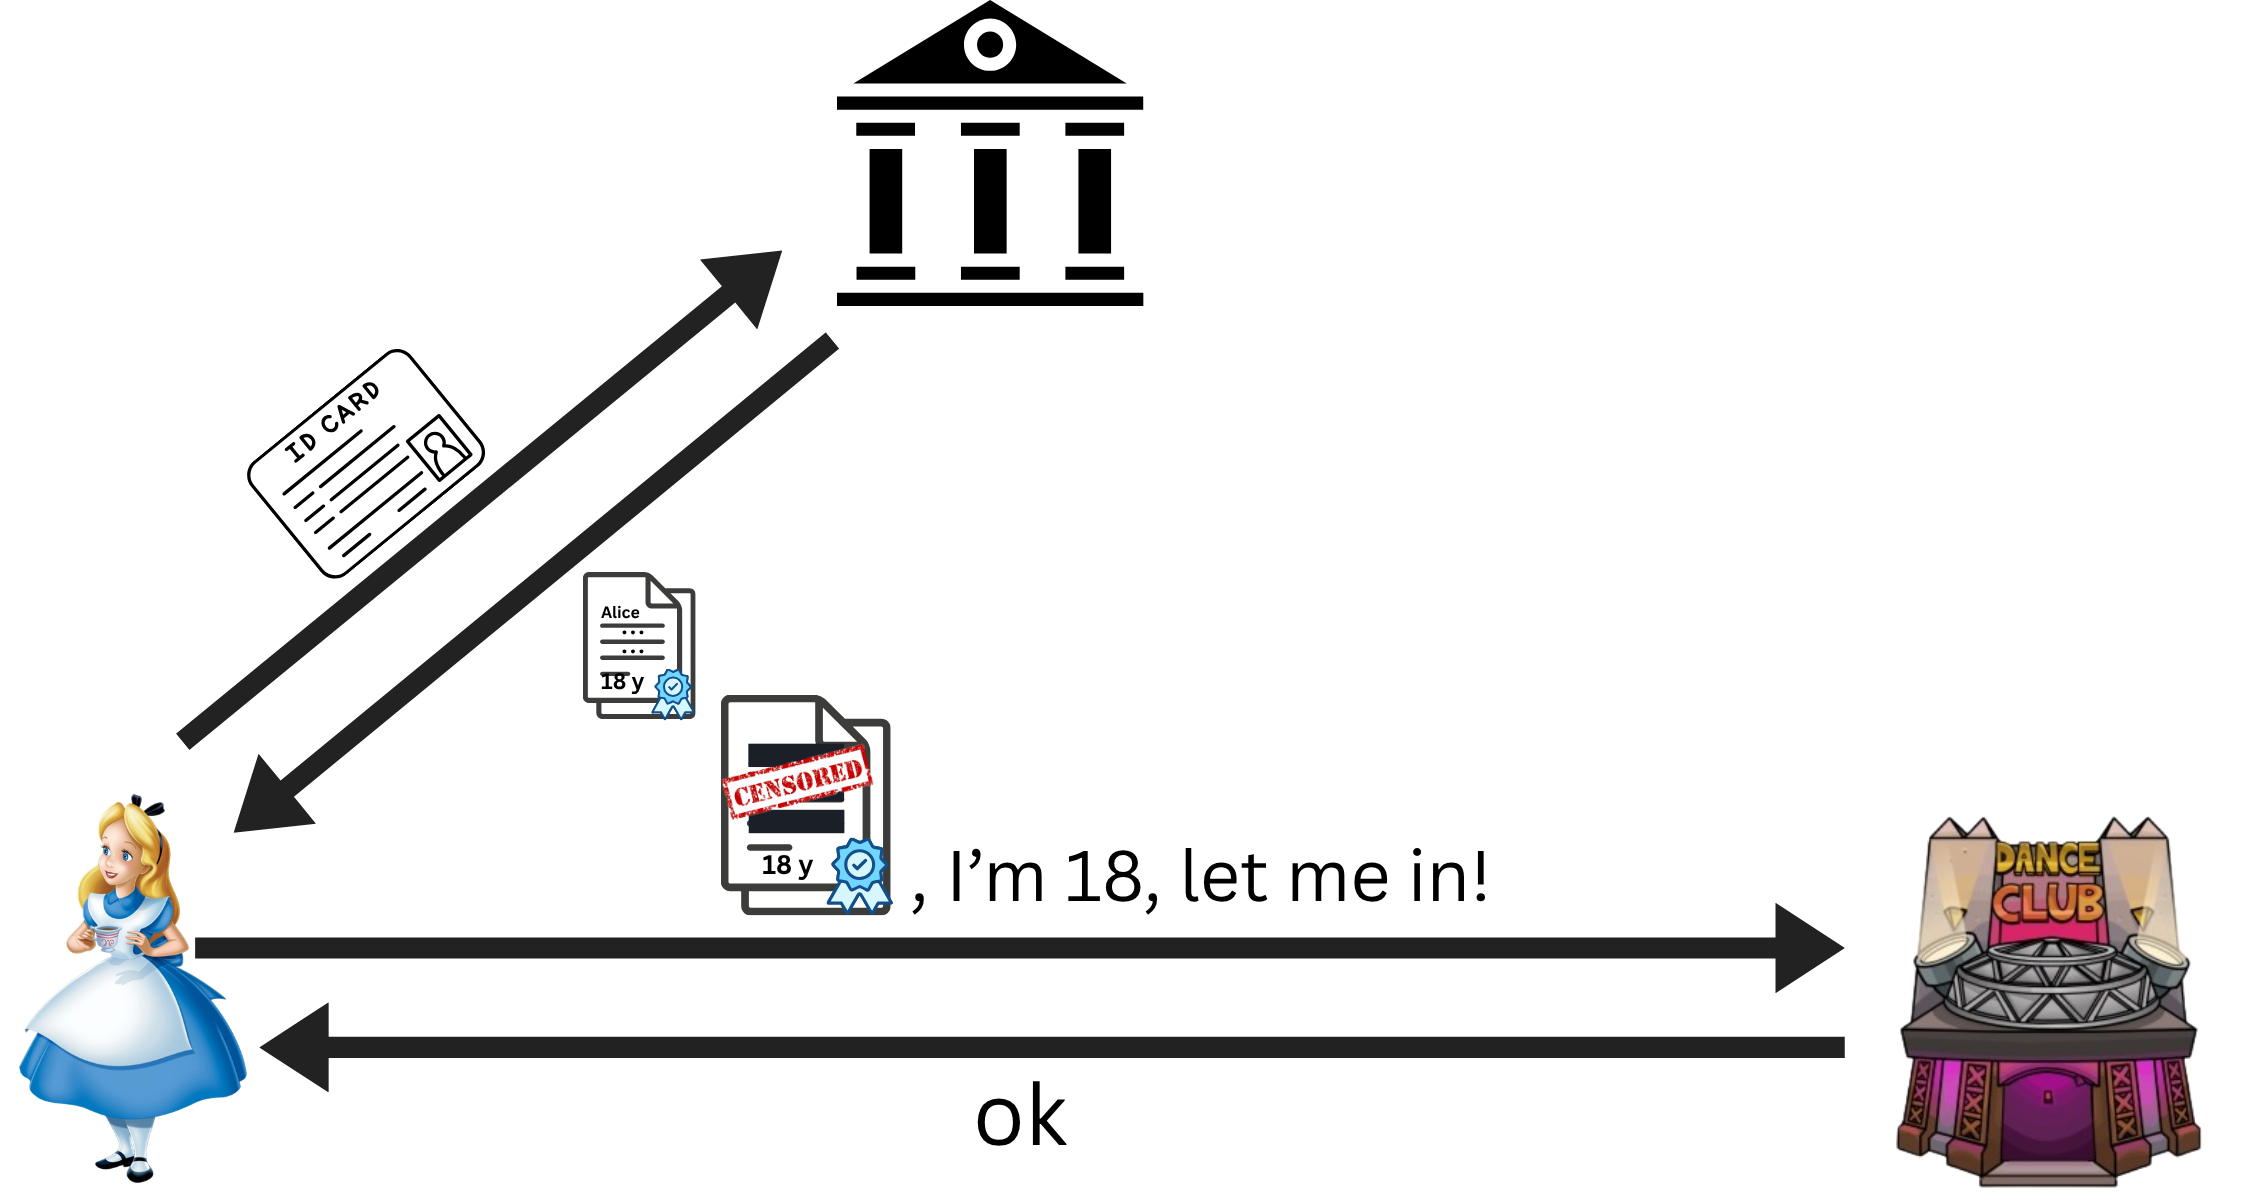
\includegraphics[width=0.8\textwidth]{figures/AnonymousCredentials.png}
    \caption{Basic scheme of anonymous credentials.}
    \label{fig:AnonymousCredentials}
\end{figure}

In the first approach~\cite{lysyanskaya2002signature},
the issuer was signing user's credentials using a secure protocol that protects user's attributes.
Credential(s) are then showed to a verifier via zero-knowledge proof of knowledge of a credential(s)
whose attributes satisfy some predicate.

Systems based on anonymous credentials have been studied and adopted over the years by big tech companies like Microsoft~\cite{paquin2013u-prove},
IBM~\cite{10.1145/586110.586114}, and are in continuous study and development by the scientific community,
facing challenges like performance improvements, revocation lists, legacy infrastructures and hardware constraints, and more recently, post quantum security.


\section{Post Quantum Transition}
\label{PostQuantumTransition}
The European union on 11 April  2024 has published a roadmap for the
post quantum digital transition of members digital infrastructures~\cite{EuropeanCommission2024PQC}.

The roadmap is a comprehensive plan that outlines the steps that each European Union member state should take in order to turn
their current infrastructure's cryptography to post-quantum secure cryptography. 
The roadmap includes a timeline for the transition, as well as a list of actions that will be taken to ensure a smooth transition.

The timeline is organized into three major phases:

\begin{enumerate}
    \item \textbf{By the end of 2026}: Initial national PQC transition roadmaps have been established by all Member States, PQC transition planning 
    and pilots for high- and medium-risk use cases have been initiated;
    \item \textbf{By the end of 2030}: The PQC transition for high-risk use cases has been completed, PQC transition planning and pilots for medium-risk
     use cases have been completed. Quantum-safe software and firmware upgrades are enabled by default.
    \item \textbf{By the end of 2035}: The PQC transition for medium-risk use cases has been completed. The PQC transition for low-risk use cases has been completed as much as feasible.
\end{enumerate}

As previously said, this roadmap has been published by the European Commission in 2024. The recent advances in the field of post-quantum computing
due to hardware improvements, artificial intelligence acceleration and advances in research have made the Q-day closer then expected, and the transition to post-quantum cryptography 
more urgent. 

On 30 March 2026, Google published a drastic advance in post-quantum cryptography: they reduced consistently the amount of time, resources and qbits needed to break  
elliptic curves based cryptography~\cite{cryptoeprint:2026/625}. In the meanwhile, between April and March 2026, big tech companies like Google~\cite{Adkins2026Google} 
and Cloudflare~\cite{Westerbaan2026Cloudflare} have announced that they will accelerate the transition to post-quantum cryptography,
lowering the timeline for the full transition to 2029, instead of 2035.

\section{Overview}
\label{overview}
In this thesis, we present a post-quantum anonymous credentials model that can be deployed with the actual technologies and legacy protocols.
We require the issuer to adopt a slightly modified version of dilithium NIST standardized post quantum signature scheme, and to slightly leverage the credentials structure in order 
to accommodate the larger size of post quantum signatures and public keys, as well as modification to the mdoc structure in order to involve a commitment
of the device public key instead of the device public key itself. 

We also provide a full open source implementation of the model. We runned our solution
implementation on different devices in different circumstances, and we provide a full 
analysis of the experimental results, showing that our solution is practical and can be 
deployed in the EUDI wallet with the actual technologies, and variation between our 
solution's performance and other realistic privacy preserving solutions are small enough 
to be acceptable in the EUDI wallet context.

In the following sections, we are going to show cryptographic primitives which are the foundations of our work~\ref{preliminaries}, we present an overview of the EUDI wallet~\ref{eudiw}, 
we perform a full analysis of the actual state of the art on device bounded anonymous 
credentials~\ref{stateoftheart}, then we explain how our solution faces and solves the challenges, performing an important advance on the actual state of the art ~\ref{oursolution}.
We show how we implemented our solution, giving a reference to our github repository~\ref{implementation}, and we present our experimental results~\ref{results}, future works that we plan to 
do~\ref{sec:future-work} and conclusion~\ref{sec:conclusion}.

\chapter{Preliminaries}
\label{preliminaries}
In this chapter, we review the basic mathematical concepts and cryptographic 
background of the thesis. We first discuss the relevant information about cryptography
and post-quantum cryptography, then hash functions, 
lattices-based cryptography, zero-knowledge proofs and commitment schemes.

\section{Group Theory}
\label{groupth}
In this section we discuss some basic concepts of group theory.
\begin{definition}[\textbf{Group}~\cite{Hoffstein2008Cryptography}]
  A group consists of a set $G$ and a rule, which we denote by $\star$,
  for combining two elements $a, b \in G$ to obtain an element $a \star b \in G$. The
  composition operation $\star$ is required to have the following three properties:
\end{definition}
\begin{itemize}
  \item \textbf{Closure Law}: For all $a,b \in G$, we have that $a\star b \in G$;
  \item \textbf{Identity Law}: There is an $e \in G$ such that 
  $e \star a = a \star e = a$ for all $a \in G$;
  \item \textbf{Inverse Law}: For every $a \in G$, there is an (unique)
  $a^{-1} \in G$ satisfying $a \star a^{-1} = a^{-1} \star a = e$;
  \item \textbf{Associative Law}: $a \star (b \star c) = (a \star b) \star c$ for all $a, b, c \in G$;
\end{itemize}
If, in addition, composition satisfies the
\begin{itemize}
    \item \textbf{Commutative Law}: For all $a, b \in G$, we have $a \star b = b \star a$.
\end{itemize}
then  the group is called a \textbf{commutative} group or an \textbf{abelian} group.

\begin{definition}[\textbf{Ring}~\cite{Huang2025GroupTheory}]
  A ring $R$ is a set that has two operations, addition and multiplication. 
  Let us denote addition and multiplication by $+$ and $\cdot$, respectively. 
  They satisfy the following properties:
\end{definition}
\begin{enumerate}
  \item \textbf{Additive commutativity}: $a + b = b + a$ for all $a, b \in R$;
  \item \textbf{Additive associativity}: $a + (b + c) = (a + b) + c$ for all $a, b, c \in R$;
  \item \textbf{Additive identity}: There exists an element $0 \in R$ such that $a + 0 = 0 + a = a$ for all $a \in R$;
  \item \textbf{Additive inverse}: For every $a \in R$, there exists an element $-a \in R$ such that $a + (-a) = (-a) + a = 0$;
  \item \textbf{Multiplicative associativity}: $a \cdot (b \cdot c) = (a \cdot b) \cdot c$ for all $a, b, c \in R$;
  \item \textbf{Distributivity}: $a \cdot (b + c) = (a \cdot b) + (a \cdot c)$ and $(a + b) \cdot c = (a \cdot c) + (b \cdot c)$ for all $a, b, c \in R$.
\end{enumerate}

Now we will introduce another important mathematical concept, which is the one
of polynomial ring, which will be used in the next sections to introduce the 
lattice problem and the dilithium signature scheme.

\begin{definition}[\textbf{Polynomial Ring}~\cite{Menezes1996Handbook}]
  If $R$ is a commutative ring, then a polynomial in the indeterminate
  $x$ over the ring $R$ is an expression of the form $$R[x] = \{a_0 + a_1x + ... + a_nx^n: n \ge 0, a_i \in R, \forall i \in \{0,1,...,n\}\}$$  
\end{definition}

The polynomial quotient ring is a class of rings in the form:$$R[x]/(f(x))$$
where $f(x)$ is some polynomial in $R[x]$.

\section{Cryptography and Post-Quantum Resistance}
\label{generalcrypto}
In this section we discuss some basic concepts of cryptography and post-quantum resistance.

Cryptography is the study of mathematical techniques related to aspects of information security 
such as confidentiality, data integrity, entity authentication, and data origin authentication~\cite{Menezes1996Handbook}.

Often, security of cryptographic schemes is defined with respect to different types of adversaries
which are classified based on their computational power and cheating capabilities, and in the
literature are called adversarial models. The most common adversarial models are show in table ~\ref{tab:adversary_types}.
\begin{table}[H]
  \centering
  \caption{Main cryptographic adversarial models~\cite{Li2024Comprehensive}.}
  \label{tab:adversary_types}
  \renewcommand{\arraystretch}{1.3}
  \begin{tabularx}{\textwidth}{|l|L|}
    \hline
    \textbf{Adversary Type} & \textbf{Description} \\ \hline
    Passive                  & Can read, copy, and analyze data. The goal is to learn confidential information. \\ \hline
    Active                   & Can read, modify, delete, and inject data. \\ \hline
    Man-in-the-middle (MITM) & Joins invisibly in a conversation between recipients. Can be passive and actively modifying conversation. \\ \hline
    Honest-but-curious       & Performs protocol correctly and attempts to learn confidential information. \\ \hline
    Fail-stop                & Can halt protocol at any time. \\ \hline
    Malicious                & Deviates from protocol entirely. \\ \hline
    Byzantine                & Coordinated malicious agents in a distributed system. \\ \hline
  \end{tabularx}
\end{table}

\subsection{Signature Schemes}

The main cryptographic primitives used for anonymous credentials systems are
signature schemes. 

\begin{definition}[\textbf{Digital Signature}~\cite{Nia2014Introduction}]
  Digital Signature is a cryptographic primitive which is
  fundamental in authentication, authorization and non-
  repudiation.
\end{definition}

A signature scheme is defined mainly by three primitive functions:
\begin{itemize}
  \item \textbf{Key Generation}: a probabilistic algorithm that generates a pair of keys, a public key and a private key;
  \item \textbf{Signing}: a probabilistic algorithm that takes as input a message and a private key, and outputs a signature;
  \item \textbf{Verification}: a deterministic algorithm that takes as input a message, a signature and a public key, and outputs a boolean value indicating whether the signature is valid or not.
\end{itemize}

As shown in Figure~\ref{fig:digsig}, when the original message is
generated by user and sent for signing, the message is
hashed and after performing key generation algorithm,
digital signature is generated and is appended to
message as “digital signature”.


\begin{figure}[ht]
  \centering
  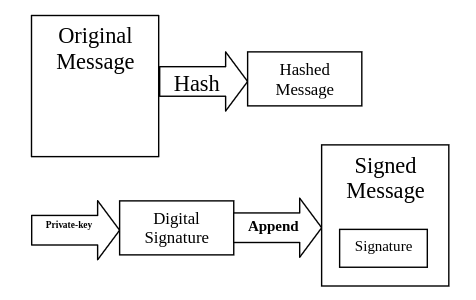
\includegraphics[width=1\textwidth]{figures/digsig.png}
  \caption{Steps of generating digital signature~\cite{Nia2014Introduction}.}
  \label{fig:digsig}
\end{figure}

In particular, the actual most efficient and widely adopted
signature scheme is ECDSA~\cite{AlZubaidie2019Efficient}, which 
stands for Elliptic Curve Digital Signature Algorithm.

\subsection{ECDSA}
ECDSA is a public key signature scheme based on the algebraic structure of 
elliptic curves over finite fields. Smartphone's secure element and
credentials issuers adopt this type of signature scheme right now.
In this section we will have a detailed overview on how ECDSA works.

\paragraph{Domain parameters}Parameters known to every party:
\begin{itemize}
  \item Elliptic curve $E$ over a finite field $\mathbb{Z}_p$
  (in our case, P-256);
  \item Numer $n = \#E(\mathbb{Z}_p)$, number of points on the curve;
  \item A generator $P\in E(\mathbb{Z})_p$;
  \item A collision-resistant hash function $H$ whose output has the same
  bitlength as $n$ (In our case, $H = $SHA256);
\end{itemize}

\paragraph{Key generation}Steps needed for Alice to generate her keypair:
\begin{itemize}
  \item Select $a \in [1,n-1]$ at random and compute $A = aP$;
  \item Alice's public key will be $A$ and her private key will be $a$;
\end{itemize}

\paragraph{Signature} To sign a message $M \in \{0,1\}^*$, Alice does the following:
\begin{enumerate}
  \item Compute $m = H(M)$ and interpret $m$ as an integer;
  \item Select a per-message secret $k \in [1,n-1]$ at random;
  \item Compute $R = kP$, then compute the $x$-coordinate of $R$, denoted as 
  $r = x(R) \mod n$ and check that $r \neq 0$. If $r = 0$, go back to step 2;
  \item Compute $s = k^{-1}(m + ar) \mod n$ and check that $s \neq 0$. If $s = 0$, go back to step 2;
  \item Alice's signature on $M$ is the pair $(r,s)$, where $r,s \in [1,n-1]$.;
\end{enumerate}
Notice that $k$ should be securely deleted after it has been used.

\paragraph{Verification} To verify a signature $(r,s)$ on a message $M$, 
Bob need to check that $s = k^{-1}(m + ar) \mod n$ holds, where $m = H(M)$ and $k$ is 
the per-message secret used by Alice to generate the signature. Bob doesn't know neither $k$ nor $a$.

Now we do the following mathematical transformations:
$$s = k^{-1}(m + ar) \mod n$$ $$\iff k \equiv s^{-1}(m + ar) \mod n$$
$$\iff k \equiv s^{-1}m + (s^{-1}r)a (\mod n)$$$$\iff k \equiv u_1 + u_2a (\mod n)$$
where $u_1 = s^{-1}m \mod n$ and $u_2 = rs^{-1} \mod n$. 

Proceedings:$$k \equiv u_1 + u_2a (\mod n)$$
$$\iff kP = (u_1 + u_2a)P$$ $$\iff kP = u_1P + u_2A$$ $$\iff R = V$$ where $V = u_1P + u_2A$;

Now recall that $R = V \iff x(R) = x(V)$ meaning that:

Bob can verify that the signature is valid by just checking
if the $x$-coordinate of $R$ is equal to the $x$-coordinate of $V$.

To verify a signature $(r,s)$ on a message $M$, Bob does the following:

\begin{enumerate}
  \item Retrieve Alice's public key $A$;
  \item Check that $r,s \in [1,n-1]$;
  \item Compute $m = H(M)$;
  \item Compute $u_1 = ms^{-1} \mod n$ and $u_2 = rs^{-1} \mod n$;
  \item Compute $V = u_1P + u_2A$ and verify that $V \neq \infty$;
  \item Finally, Bob accepts the signature ($M,(r,s)$) if and only if $x(R) = x(V)$.
\end{enumerate}

The problem with ECDSA is that elliptic curve cryptography is based on the
discrete logarithm problem, which can be solved in polynomial time by a 
quantum computer using Shor's algorithm~\cite{Shor1997Polynomial}.

In order for our thesis to be post-quantum secure, we need to adopt a 
post-quantum secure signature scheme.

Since Shor's algorithm has been discovered in 1997, many post-quantum
signature schemes have been proposed and some of them have been standardized
by NIST. In this table we represent the main NIST standardized post-quantum 
signature schemes, their underlying problem and a brief explanation of how 
they work~\ref{tab:pqc_signatures}.

\begin{table}[H]
  \centering
  \caption{NIST Standardized Post-Quantum Signature Schemes~\cite{NIST_FIPS_204}.}
  \label{tab:pqc_signatures}
  \small
  \renewcommand{\arraystretch}{1.3}
  \begin{tabularx}{\textwidth}{|l|l|L|L|}
    \hline
    \textbf{Scheme} & \textbf{Standard} & \textbf{Underlying Problem} & \textbf{Brief Explanation} \\ \hline
    \textbf{ML-DSA} (Dilithium)~\cite{NIST2024FIPS204} & FIPS 204       & Module Learning with Errors (MLWE) \& Module Short Integer Solution (MSIS) & Based on the ``Fiat-Shamir with Aborts'' framework. It creates a signature by generating a commitment and response, applying rejection sampling to ensure the output does not leak information about the private key. \\ \hline
    \textbf{SLH-DSA} (SPHINCS+)~\cite{NIST2024FIPS205} & FIPS 205       & Collision and pre-image resistance of cryptographic hash functions       & A stateless hash-based signature scheme. It uses a hyper-tree of Merkle trees to authenticate underlying one-time (WOTS+) and few-time (FORS) signature key pairs. \\ \hline
    \textbf{FN-DSA} (FALCON)~\cite{Prest2024Falcon}    & Draft FIPS 206 & NTRU Lattice Problem                                                     & Uses a hash-and-sign framework with fast-Fourier sampling over NTRU lattices. It produces highly compact signatures, though the signing process requires complex floating-point arithmetic. \\ \hline
  \end{tabularx}
\end{table}

In Section~\ref{dilithium} we are going to discuss in depth the Dilithium signature scheme, 
which is the one we adopted for our post-quantum anonymous credentials model.

\section{Hash Functions}
\label{hashfunctions}
Hashing  is  a  fundamental  concept  in 
cryptography,  playing  a  vital  role  in  ensuring 
data  integrity, authenticity, and  security.

\begin{definition}[\textbf{Hash Function}~\cite{inproceedings}]
  A hash function is a mathematical function that takes in input data
  of arbitrary size and maps them into a fixed-size output, known as
  hash value.
\end{definition}

\subsection{Cryptographic Hash Functions}
\label{cryptohashfunction}

In cryptography, a particular family of hash functions called 
\textbf{cryptographic hash functions} is used in order to ensure 
data  integrity,  secure  information,  and  enable 
efficient data retrieval.

There are several properties that a cryptographic hash function must satisfy:
\begin{itemize}
  \item \textbf{Deterministic output}: The same input will always produce the same output;
  \item \textbf{Collision resistance}: It should be computationally infeasible to find two 
  different inputs that produce the same output;
  \item \textbf{Pre-image resistance}: Given a hash value, it should be computationally infeasible 
  to find the original input;
  \item \textbf{Second pre-image resistance}: Given an input and its hash value, it should 
  be computationally infeasible to find a different input that produces the same hash value;
  \item \textbf{Avalanche effect}: A small change in the input should produce a significantly 
  different output.
\end{itemize}

\subsection{SHA-2 Family}
\label{sha2} 
The Secure Hash Algorithm 2 (SHA-2) family is a set of cryptographic hash functions
published by the National Institute of Standards 
and Technology (NIST) in 2002~\cite{NIST2002FIPS1802}.
The SHA-2 architecture comprises the following key components:
\begin{itemize}
  \item \textbf{Hash function}: The core functionality that process a message
  and generates a fixed size output, iteratively applying compression functions;
  \item \textbf{Message schedule}: The process of dividing the input message into 
  fixed-size blocks and preparing them for processing;
  \item \textbf{Compression function}: The function that process a fixed-size block
  and a current state in order to produce a new state;
  \item \textbf{Padding scheme}: The process of adding extra bits to the input message 
  to ensure that its length is a multiple of the block size.
\end{itemize}
In the SHA-2 family, the most commonly used hash functions are SHA-256 and SHA-512, 
which produce 256-bit and 512-bit hash values, respectively.


\subsection{Poseidon Hash Function}
\label{poseidon}
The Poseidon hash functions are hash functions designed  for the use in 
verifiable computation protocols. 
There are several different version of the specification:
\begin{itemize}
  \item First version: \textbf{Usenix Poseidon}~\cite{Grassi2021Poseidon};
  \item Second version: \textbf{Eurocrypt Poseidon}~\cite{cryptoeprint:2023/323};
  \item Third version: \textbf{Poseidon22}~\cite{10.1007/978-3-031-37679-5_8}, which is
  an optimized, faster version.
\end{itemize}
His key design goals are:
\begin{itemize}
  \item \textbf{ZK-friendliness}: Efficient inside arithmetic circuits (low R1CS/constraint cost).
  \item \textbf{Security}: Cryptographically strong against preimage, collision, and other standard attacks.
  \item \textbf{Flexibility}: Parameterizable for different field sizes, security levels, and performance needs.
\end{itemize}
In particular, in our work we are going to use the Poseidon2 (also called Poseidon23) version, 
which is the one that is used in the zk-dilithium STARK zero-knowledge 
proof system.

\section{Commitment Schemes}
\label{commitments}
A commitment scheme is a cryptographic primitive that allows a party to commit to a value 
while keeping it hidden, with the ability to reveal the committed value later. 
Commitment schemes are widely used in various cryptographic protocols, including zero-knowledge proofs, 
secure multi-party computation, and digital signatures. In the picture~\ref{fig:commitment}
a simple representation of a commitment scheme is shown.

\begin{figure}
  \centering
  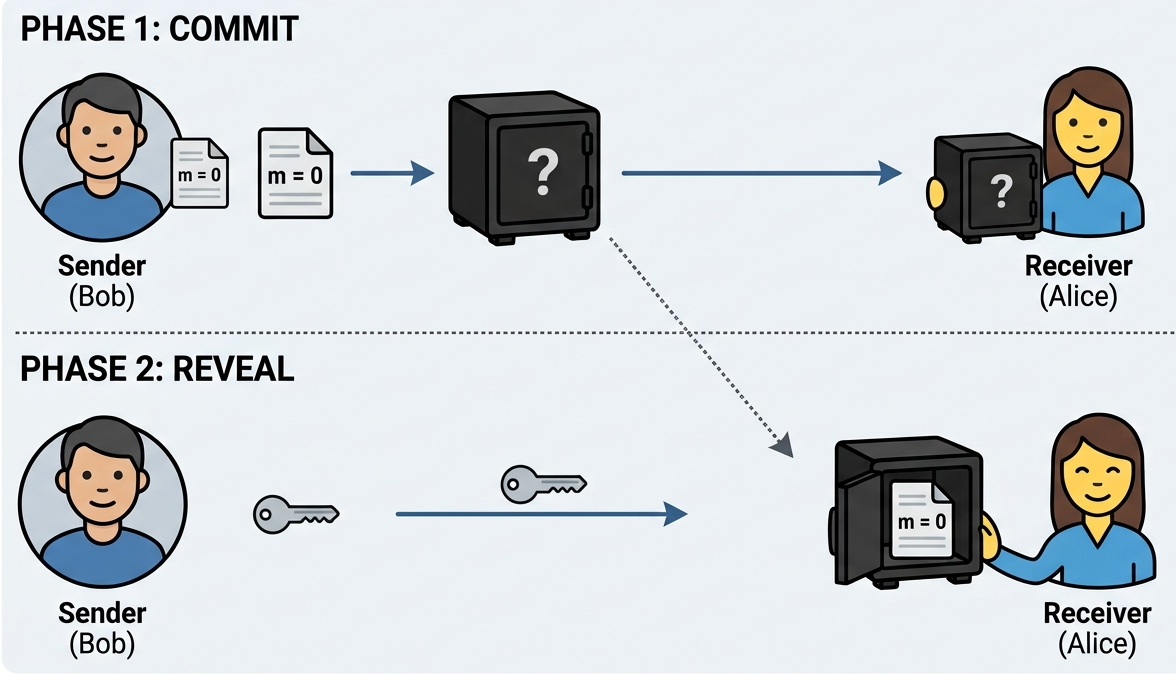
\includegraphics[width=0.8\textwidth]{figures/commitment.png}
  \caption{Commitment scheme representation.}
  \label{fig:commitment}
\end{figure}

Commitment schemes have two main properties:

\begin{itemize}
      \item \textbf{Binding}: The binding property dictates that once the commitment is sent, the committer cannot alter the underlying 
      message~\cite{Damgard1999}.We need the commitment to be associated to a single credential in order not to allow a malicious
      prover to build the two different proofs over two different credentials;
      \item \textbf{Hiding}: The hiding property ensures that when a commitment is sent, the receiver learns absolutely nothing about 
      the underlying secret value~\cite{Damgard1999}. We need our commitment to be hiding, and in particular to involve some randomness,
      because if the commitment is deterministic, then the prover's commitment across different presentations of the same credential
      would be the same, and this would allow the verifier to link different presentations of the same credential.
\end{itemize}

\section{MAC}
\label{mac}

MAC (Message Authentication Code) is a cryptographic primitive that provides data 
integrity and authenticity. It is a short piece of information used to authenticate 
a message and to provide integrity and authenticity assurances on the message~\cite{Paar2024}. 

A MAC algorithm takes as input a secret key and a message, and outputs a MAC value (also called a tag). 
The MAC value is then sent along with the message to the receiver, who can use the same secret key to 
verify the authenticity and integrity of the message. A simple representation of a how a MAC is used
is shown in figure~\ref{fig:mac}.

\begin{figure}
  \centering
  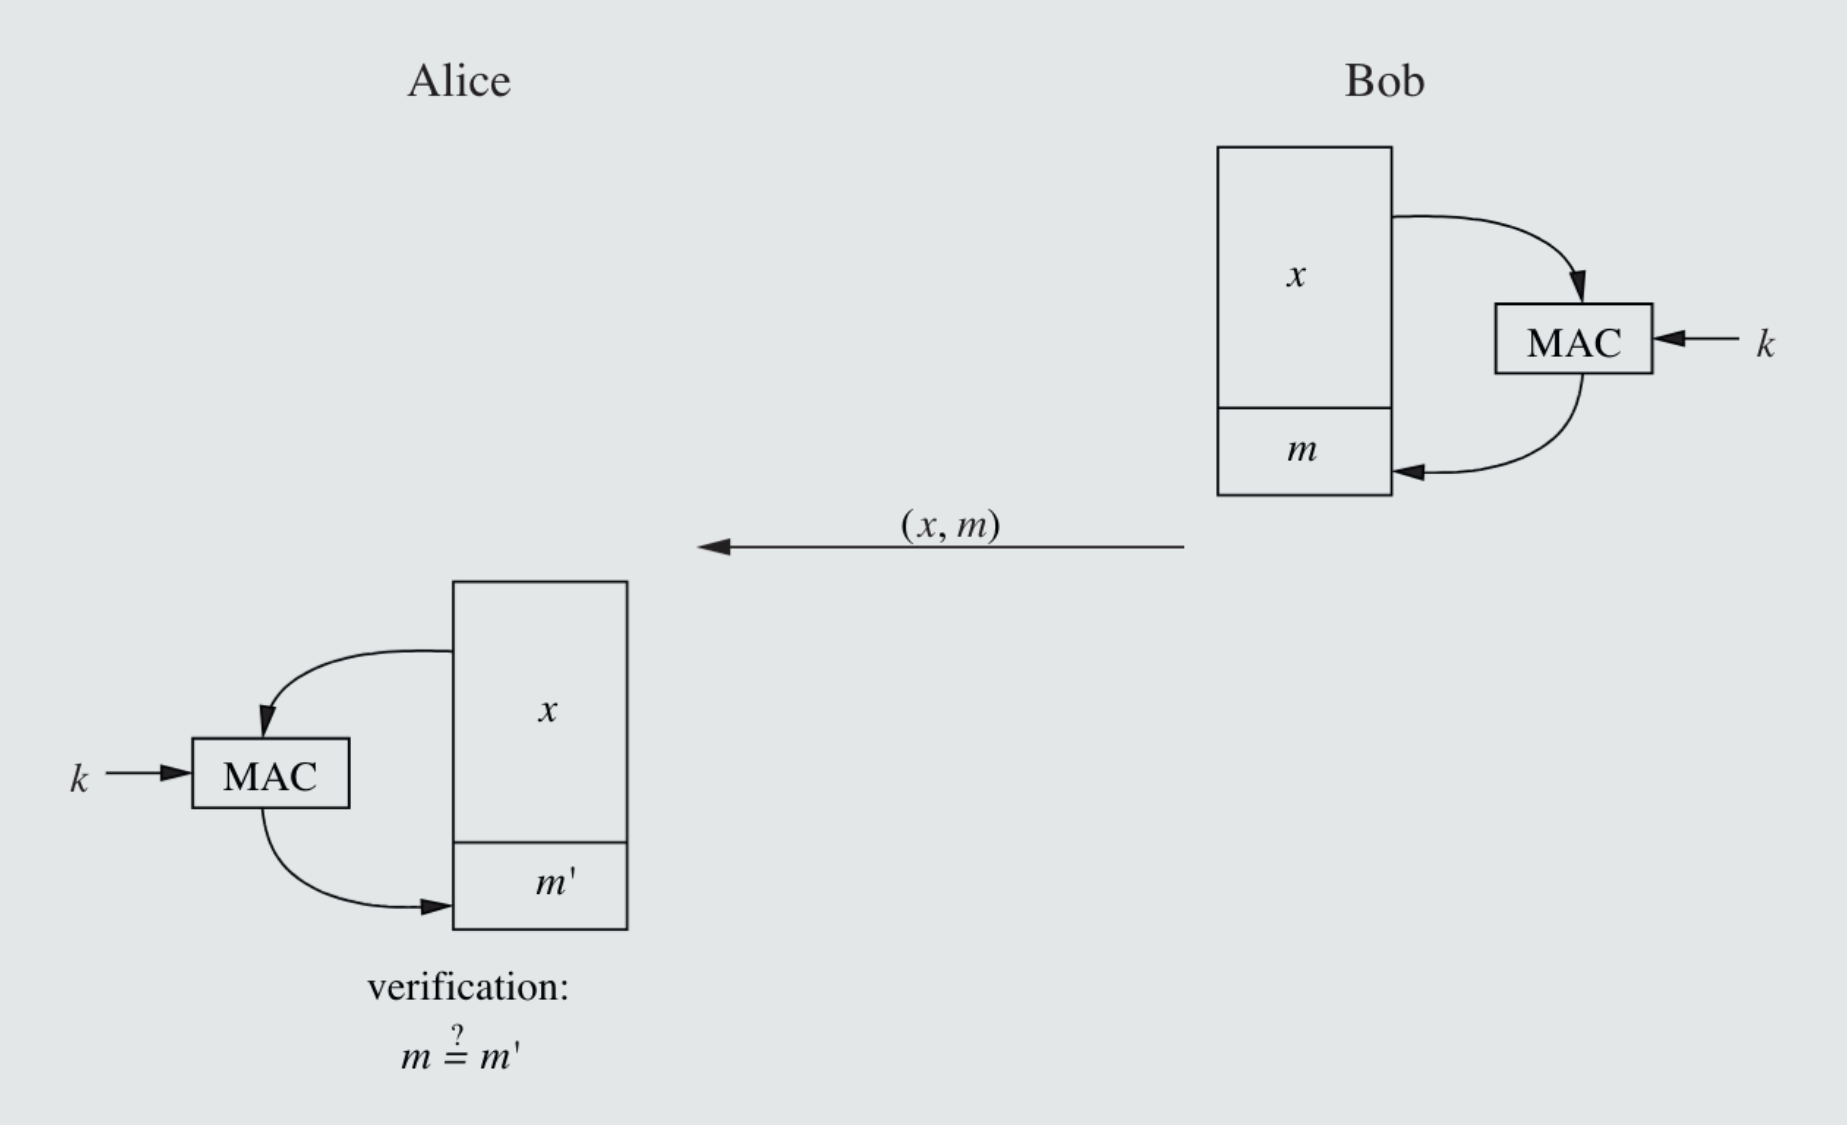
\includegraphics[width=0.8\textwidth]{figures/mac.png}
  \caption{MAC representation.}
  \label{fig:mac}
\end{figure}

The most basic MAC construction that we will take in consideration
in this thesis is the information-theoretic secure MAC.
Computed on a message $m$, the information-theoretic secure MAC is defined as: $$m = a*m + b (\mod n)$$
where $a$ and $b$ are secret keys, and the operations are performed in a finite field $\mathbb{F}_q$.

\section{Lattice Problem}
Notice that $\mathbb{Z}_q = \{0, 1, \ldots, q-1\}$ and $x \in_{R}S$ means that $x$ is sampled uniformly at random from the set $S$.

\label{lattice}
\begin{definition}[\textbf{Lattice}]
  Let $v_1,...,v_n\in \mathbb{R}^m$ be a set of linearly independent vectors.
  The lattice L generated by $v_1,...,v_n$ is the set of linear combinations of
  $v_1,...,v_n$ with coefficients in $\mathbb{Z}$:$$L = \{a_1v_1 + a_2v_2+\cdots +a_nv_n : a_i \in \mathbb{Z} \}$$
\end{definition}
Informally, a lattice is a set of points in m-dimension space with periodic structure.
A simple 2-dimensional representation of a lattice is shown in figure~\ref{fig:lattice}.
\begin{figure}
  \centering
  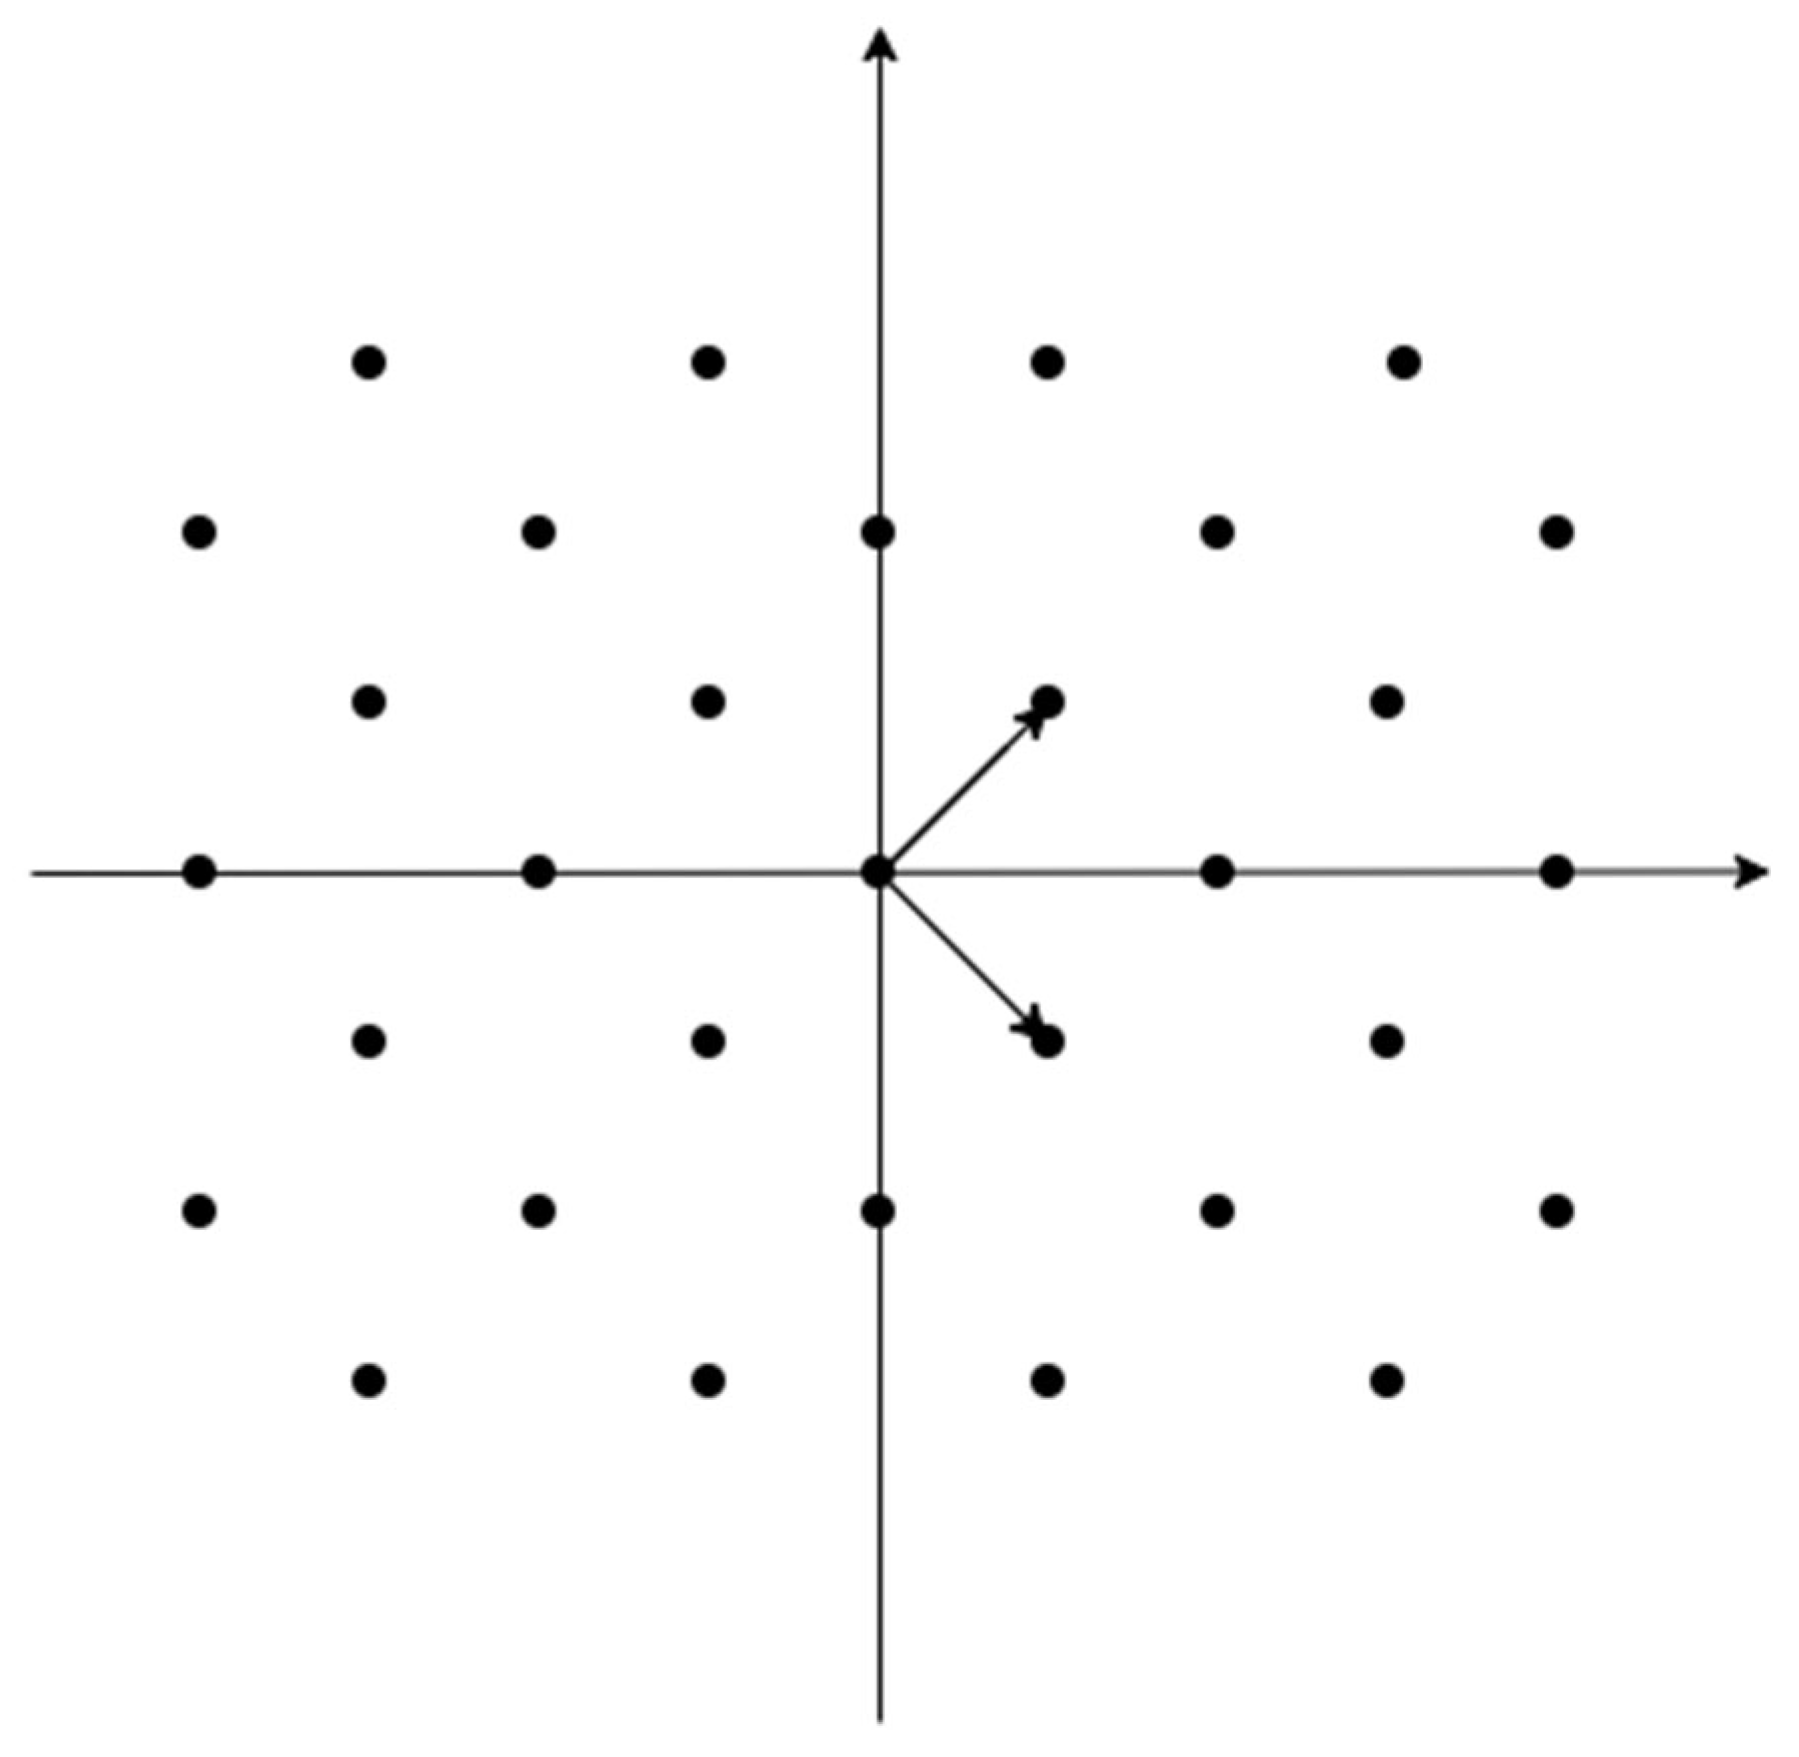
\includegraphics[width=0.7\textwidth]{figures/lattice.png}
  \caption{A simple 2-dimensional lattice}
  \label{fig:lattice}
\end{figure}

Suppose that $v_1,...,v_n$ is a basis for a lattice L and that $w_1,...,w_n\in L$
is another collection of vectors in L.

We can write each $w_j$ as linear combination of the basis vectors:
$$w_1 = a_{1,1}v_1 + a_{1,2}v_2+\cdots +a_{1,n}v_n$$
$$w_2 = a_{2,1}v_1 + a_{2,2}v_2+\cdots + a{2,n}v_n$$
$$\vdots$$
$$w_n = a_{n,1}v_1 + a_{n,2}v_2+\cdots + a_{n,n}v_n$$

Suppose now that we want to express $v_i$ in terms of $w_j$, then we
should invert the matrix 
$$A = \begin{pmatrix} a_{1,1} & a_{1,2} & \cdots & a_{1,n} \\ a_{2,1} & a_{2,2} & \cdots & a_{2,n} \\ \vdots & \vdots & \ddots & \vdots \\ a_{n,1} & a_{n,2} & \cdots & a_{n,n} \end{pmatrix}$$
Since we are dealing with lattices, we need the coefficients of $A^{-1}$ to be integers.
Hence, we will have $det(A) = det(A^{-1}) = \pm 1$.
Conversely, if $det(A) = \pm 1$, then $A^{-1}$ has integer coefficients by theory
of adjoint matrix.
So we can state that any two bases for a lattice L are related by a matrix having 
integer coefficients and determinant $\pm 1$.

Recalling the definition of Euclidean norm as $$||v|| = \sqrt{\sum_{i = 1}^{n}v_i^2},\ v \in \mathbb{R}^n$$
there are 2 fundamental problems in lattice-based cryptography~\cite{Hoffstein2008Cryptography}:
\begin{definition}[\textbf{Shortest Vector Problem (SVP)}]
  Find a shortest non-zero vector
  in a given lattice L, i.e. a non zero vector that minimizes the Euclidean norm $||t||$.
\end{definition}

\begin{definition}[\textbf{Closest Vector Problem (CVP)}]
  Given a vector $w \in \mathbb{R}^m$ that is not
  in $L$, find a vector $v \in L$ that is closest to $w$, i.e. a vector $v \in L$ that minimizes 
  the Euclidean norm $||w-v||$.
\end{definition}

\subsection{Short Integer Solution (SIS)}
\label{sis}

\begin{definition}[\textbf{SIS}$_{n,m,q,\beta}$~\cite{Ajtai1996Generating}]
  Let $n, m, q$ be positive integers and $\beta \ll {q\over 2}$ a real bound. Given a uniformly random matrix $\mathbf{A} \in \mathbb{Z}_q^{n \times m}$, find a \emph{non-zero} integer vector $\mathbf{z} \in \mathbb{Z}^m$ such that
  $$Az = 0 \pmod{q} \quad \text{and} \quad z \in [-\beta, \beta]^m.$$
\end{definition}

$\mathbf{A}$ is a random matrix with $n$ rows and $m$ columns, where $n < m$; we are looking for a short, non-trivial combination of its columns that sums to zero modulo $q$. When $\beta$ is much smaller than $q$, finding such a vector is believed to be computationally hard even for quantum computers. The SIS assumption is the foundation for collision-resistant hash functions 
and for the \emph{unforgeability} of lattice-based signatures, including Dilithium.

\subsection{Module-SIS (M-SIS)}
\label{msis}

The \textbf{Module-SIS} problem is the algebraic generalization of SIS to polynomial rings, which is the setting used by Dilithium (ML-DSA).

\begin{definition}[\textbf{M-SIS}$_{n,k,\ell,q,\beta}$~\cite{Langlois2015Worst}]
  Given $a_1,a_2,\cdots,a_{\ell}\in_{R}\mathbb{R}^k_q$ where ($\ell > k$), find $z_1,z_2,\cdots,z_{\ell}\in \mathbb{R}_q$ such
  that $a_1z_1 + a_2z_2 + \cdots + a_{\ell}z_{\ell} = 0$ where $\|z_i\|_{\infty} \le \beta$ and
  not all $z_i$ are $0$.
\end{definition}

The key advantage of working over a polynomial ring is \emph{compactness}: a single polynomial in $R_q$ of degree $n-1$ packs $n$ integers, so keys and signatures are much smaller than in plain SIS with the same security level. M-SIS is at least as hard as SVP on ideal lattices, which inherit the worst-case hardness guarantees of standard SIS~\cite{Langlois2015Worst}. The unforgeability of Dilithium signatures reduces to M-SIS.

\subsection{Learning With Errors (LWE)}
\label{lwe}

\begin{definition}[\textbf{LWE}$_{n,m,q,\beta}$~\cite{Regev2005Lattices}]
  Let $n, m$ be positive integers ,$q$ be a prime number and $\beta \ll {q\over 2}$. Let $s\in_{R} \mathbb{Z}^n_q$ and
  $e \in_{R}[-\beta,\beta]^m$.

  Given $A\in_{R} \mathbb{Z}^{m\times n}_q$ and $b = As + e\ (mod\ q)\in \mathbb{Z}^m_q$, find $s$.

\end{definition}

Intuitively, the problem looks like a noisy system of linear equations: if there were no errors $e_i$, recovering $\mathbf{s}$ would be easy. Adding small errors makes the problem hard. Regev showed~\cite{Regev2005Lattices} that LWE is as hard as approximating certain lattice problems in the worst case, even for quantum algorithms. LWE underlies the \emph{hiding} property of lattice-based encryption and key-encapsulation mechanisms, and contributes to the binding property of Dilithium commitments.

\subsection{Module-LWE (M-LWE)}
\label{mlwe}

Exactly as M-SIS generalizes SIS, \textbf{Module-LWE} generalizes LWE to the polynomial ring $R_q = \mathbb{Z}_q[x]/(x^n+1)$.

\begin{definition}[\textbf{M-LWE}$_{n,k,\ell,q,\beta}$~\cite{Langlois2015Worst}]
  Let $s\in_{R} \mathbb{R}^{\ell}_q$ and $e\in_{R}S^k_{\beta}$ where $k > \ell$ and $\beta \ll {q\over 2}$.
  Let $a_1,a_2,\cdots,a_k\in_{R}\mathbb{R}^{\ell}_q$ and $b_i = a^T_is + e_i\in \mathbb{R}$ for $i = 1,\cdots,k$.
  Given the $a_i$ and $b_i$, determine $s$.
\end{definition}

M-LWE inherits the worst-case hardness of LWE, now over module lattices~\cite{Langlois2015Worst}. In Dilithium (ML-DSA), the public key is an M-LWE sample $\mathbf{t} = \mathbf{A}\mathbf{s}_1 + \mathbf{s}_2$: recovering the secret vectors $(\mathbf{s}_1, \mathbf{s}_2)$ from $(\mathbf{A}, \mathbf{t})$ is exactly an instance of M-LWE, so the scheme's key indistinguishability and simulation security both rest on this assumption.

\subsection{Dilithium}
\label{dilithium}
In this section we are going to provide a simplified version of the Dilithium signature scheme,
in order to give a complete overview of the cryptographic primitives used in our post-quantum anonymous credentials model.

We will focus on the key generation, signing and verification algorithms, and we will provide a brief overview of the security properties of the scheme,
relying on reductions on previously defined lattice problems, in particular M-SIS and M-LWE.

This simplified version has been taken from Prof. Menezes' book~\cite{Menezes1996Handbook}.

\paragraph{Notation and parameters} In the table~\ref{tab:mldsa_parameters} we summarize the main notation and parameters used in the Dilithium signature scheme specification
that we are going to show. The parameters are defined in the Dilithium NIST specification~\cite{NIST2024FIPS204} and are chosen to achieve a specific security level, as defined in the NIST post-quantum cryptography standardization process.

\begin{table}[H]
  \centering
  \caption{FIPS 204 parameter sets for Dilithium (ML-DSA).}
  \label{tab:mldsa_parameters}
  \small
  \renewcommand{\arraystretch}{1.3}
  \begin{tabularx}{\textwidth}{|c|X|c|c|c|}
    \hline
    \textbf{Parameter} & \textbf{Description} & \textbf{ML-DSA-44} & \textbf{ML-DSA-65} & \textbf{ML-DSA-87} \\ \hline
    $q$ & Prime modulus & $2^{23} - 2^{13} + 1$ & $2^{23} - 2^{13} + 1$ & $2^{23} - 2^{13} + 1$ \\ \hline
    $n$ & Ring degree for $R_q = \mathbb{Z}_q[x]/(x^n + 1)$ & 256 & 256 & 256 \\ \hline
    $(k, \ell)$ & Dimensions of matrix $A$ & (4,4) & (6,5) & (8,7) \\ \hline
    $\eta$ & Coefficient bound for $s_1, s_2$ & 2 & 4 & 2 \\ \hline
    $\gamma_1$ & Coefficient bound for $y$ & $2^{17}$ & $2^{19}$ & $2^{19}$ \\ \hline
    $\tau$ & Number of 1's in $c$ & 39 & 49 & 60 \\ \hline
    $\beta$ & $\beta = \tau\eta$ & 78 & 196 & 120 \\ \hline
    $\gamma_2$ & HighBits/LowBits parameter & $(q - 1)/88$ & $(q - 1)/32$ & $(q - 1)/32$ \\ \hline
    $\alpha$ & $\alpha = 2\gamma_2$ & $(q - 1)/44$ & $(q - 1)/16$ & $(q - 1)/16$ \\ \hline
    $\lambda$ & Collision strength of $\tilde{c}$ & 128 & 192 & 256 \\ \hline
    $d$ & Number of dropped bits from $t$ & 13 & 13 & 13 \\ \hline
    $\omega$ & Maximum number of 1's in hint vector & 80 & 55 & 75 \\ \hline
    $\Lambda$ & Security level & $\approx 128$ & $\approx 192$ & $\approx 256$ \\ \hline
  \end{tabularx}
\end{table}

Moreover, we define the following notation that we are going to adopt in the Dilithium signature scheme specification:
\begin{itemize}
  \item $\mathbb{Z}_q$ is the set of integers modulo $q$;
  \item $R_q$ is the ring $\mathbb{Z}_q[x]/(x^n + 1)$;
  \item $S_{\eta}$ is the set of polynomials in $R_q$ with coefficients in $[-\eta, \eta]$;
  \item $S_{\gamma_1}$ is the set of polynomials in $R_q$ with coefficients in $(-\gamma_1, \gamma_1]$;
  \item $(k, \ell)$ are the dimensions of the matrix $A$, with $k > \ell$;
  \item $B_{\tau}$ is the set of polynomials in $S_1$, exactly $\tau$ of whose coefficients are $\pm 1$;
  \item $\beta = \tau\eta$.
\end{itemize}

Now we will proceed to show how the three key generation, signature and verification algorithms works.

\paragraph{Key generation} To generate a key pair, the following steps are performed:
\begin{enumerate}
  \item Select $A\in R_q^{k\times \ell}$ uniformly at random;
  \item Sample $s_1\in_{R}S_{\eta}^{\ell}$ and $s_2\in_{R}S_{\eta}^{k}$ uniformly at random;
  \item Compute $t = As_1 + s_2$;
\end{enumerate}
The generation is terminated. Alice's public key is $(A, t)$ and her private key is $(s_1, s_2)$.
Notice that computing $s_1$ from $(A, t)$ is an instance of the \textbf{M-LWE problem}.

\paragraph{Signature}To sign a message $M \in \{0, 1\}^*$, the following steps are performed:
\begin{enumerate}
  \item Found = false;
  \item While not Found:
  \begin{enumerate}
    \item Sample $y\in_{R}S_{\gamma_1}^{\ell}$ uniformly at random;
    \item Compute $w = Ay$ and $w_1 = HighBits(w)$;
    \item Compute $c = H(M\|w_1)$;
    \item Compute $z = y + cs_1$;
    \item If LowBits($w - cs_2$) are sufficiently small then found = true;
    \end{enumerate}
  \item Output the signature $\sigma = (z, c)$.
\end{enumerate}
Signing a message might take several iterations, but with careful parameter selection
there is an high probability that the LowBits are sufficiently small.
This rejection project is needed in order to ensure that the verifier
is actually able to verify the signature while not being able to compute $w$.

\paragraph{Verification} To verify a signature $\sigma = (z, c)$ on a message $M$, the following steps are performed:
\begin{enumerate}
  \item Obtain an authentic copy of Alice's public key $(A, t)$;
  \item Compute $w' = Az - ct$ and $w'_1 = HighBits(w')$;
  \item Compute $c' = H(M\|w'_1)$;
  \item If $c' = c$ then accept the signature, otherwise reject it.
\end{enumerate}

M-SIS guarantees unforgeability: It ensures that an adversary who does not know the secret key cannot manufacture a fake signature that a verifier will accept.



\section{Zero-Knowledge Proofs}
\label{zkproofs}
In this section we are going to provide a brief overview of the zero-knowledge proofs, 
which are a fundamental building block of our post-quantum anonymous credentials model.
We are also going to provide a brief overview of the main zero-knowledge proof systems 
that are used in our model.

\begin{definition}[\textbf{Zero-knowledge proof}]
  A zero-knowledge proof, or ZKP, is a cryptographic method that allows a/multiple verifier(s) 
  to verify a statement’s truth without revealing information beyond the statement itself. 
\end{definition}

Zero-knowledge proofs were formally introduced in 1985 by Goldwasser, Micali
and Rackoff~\cite{Goldwasser1989Knowledge}, who defined the three fundamental properties of zero-knowledge proofs:
\begin{itemize}
  \item \textbf{Completeness}: The completeness property ensures that
  an honest prover can always convince an honest verifier;
  \item \textbf{Soundness}: The soundness property ensures that a 
  dishonest prover cannot convince a verifier of a false statement, except with
  negligible probability;
  \item \textbf{Zero-knowledge}: The zero-knowledge property ensures that the verifier 
  learns nothing about the statement being proven, except for its validity.
\end{itemize}
Zero-knowledge proofs are a widely adopted tool in the actual cryptography landscape,
finding their application in many different fields, such as privacy-preserving authentication,
blockchain, and secure multi-party computation.

During the last decades, many different zero-knowledge proof systems have been proposed,
each of them with different properties and trade-offs, and different underlying mathematical problems.

In the table~\ref{tab:zk_systems_trusted_setup}, we summarize the main zero-knowledge proof systems that are used
in the actual cryptography landscape, with their underlying mathematical problem and need of trusted setup,
emphasizing their post-quantum security.

\begin{table}[H]
  \centering
  \caption{Trusted Setup and Post-Quantum Security Status of Core Zero-Knowledge Frameworks.}
  \label{tab:zk_systems_trusted_setup}
  \footnotesize
  \renewcommand{\arraystretch}{1.3}
  \begin{tabularx}{\textwidth}{|>{\raggedright\arraybackslash}p{0.11\textwidth}|>{\raggedright\arraybackslash}p{0.16\textwidth}|L|>{\raggedright\arraybackslash}p{0.19\textwidth}|>{\centering\arraybackslash}p{0.09\textwidth}|}
    \hline
    \textbf{Framework} & \textbf{Authors \& Release} & \textbf{Underlying Problem} & \textbf{Trusted Setup} & \textbf{PQ Sec.} \\ \hline
    \textbf{STARK}~\cite{BenSasson2018STARK} & Ben-Sasson et al.\ (2018) & Interactive Oracle Proofs (IOP) \& Fast Reed-Solomon Proximity Testing (FRI) & None (Transparent) & Secure \\ \hline
    \textbf{LIGERO}~\cite{Ames2017Ligero}    & Ames et al.\ (2017)       & Hardness of decoding random linear codes / Interleaved Reed-Solomon Codes & None (Transparent) & Secure \\ \hline
    \textbf{Groth16}~\cite{cryptoeprint:2016/260} & Groth (2016)         & Discrete Logarithm \& Bilinear Pairings on Elliptic Curves (over QAPs) & Required (Circuit-Specific) & Vulnerable \\ \hline
    \textbf{Plonk}~\cite{Gabizon2019Plonk}   & Gabizon et al.\ (2019)    & Polynomial Commitment Schemes (KZG Pairings) \& Grand Product Arguments & Required (Universal \& Updatable) & Vulnerable \\ \hline
    \textbf{RISC Zero}~\cite{RiscZero2026}   & RISC Zero Team (2022)    & RISC-V ISA Emulation \& STARK Protocol (DEEP-ALI) & None (Transparent) & Secure \\ \hline
    \textbf{Halo 2}~\cite{Hopwood2021Halo2}  & Hopwood et al.\ (2021)   & Discrete Logarithm over Cycles of Elliptic Curves (Pasta Curves) / IPA & None (Transparent) & Vulnerable \\ \hline
  \end{tabularx}
\end{table}

For our implementation of post-quantum anonymous credentials, we are going to use the Ligero and STARK zero-knowledge proof systems, 
which are both post-quantum secure and have public libraries adapted to our needs.

\subsection{Ligero}
\label{Ligero}
Ligero is a zero-knowledge proof system proposed in 2017 by Ames et al.~\cite{Ames2017Ligero}.
Ligero is based on the following advanced cryptographic techniques:
\begin{itemize}
  \item \textbf{MPC-in-the-Head}~\cite{10.1145/1250790.1250794}: MPC-in-the-Head, which stands for Multi-Party Computation in the Head, is
  a cryptographic protocol which allows a prover to build a zero-knowledge proof by simulating a multi-party computation (MPC) protocol in 
  their own head, without actually communicating with other parties. The prover generates multiple views of the computation, each corresponding 
  to a different party's perspective, and then commits to these views. The verifier can then challenge the prover to reveal all but one view, 
  allowing them to check the correctness of the computation without learning any sensitive information. Repeating the process a certain amount
  of times allows the verifier to establish that the success probability of a cheating prover is negligible. A visual representation of the 
  MPC-in-the-Head technique is shown in figure~\ref{fig:mpcinthehead}. 
  \item \textbf{Interleaved Reed-Solomon Codes}~\cite{Ames2017Ligero}: Reed-Solomon codes function by mapping a message of length $k$ to
  the coefficients of a polynomial $P(x)$ of degree at most $k-1$, which is then evaluated at $n$ distinct points ($n > k$). This generates
  an $n$-length codeword where the inherent algebraic redundancy ensures that any two distinct codewords differ in at least $n - k + 1$
  positions. In Ligero, the prover encodes witness values into a matrix whose rows are Reed-Solomon codewords; this \emph{interleaved}
  structure enables efficient batch verification through random column sampling, which detects any cheating prover with high probability
  by exploiting the large minimum distance of the code.
\end{itemize}

\begin{figure}
  \centering
  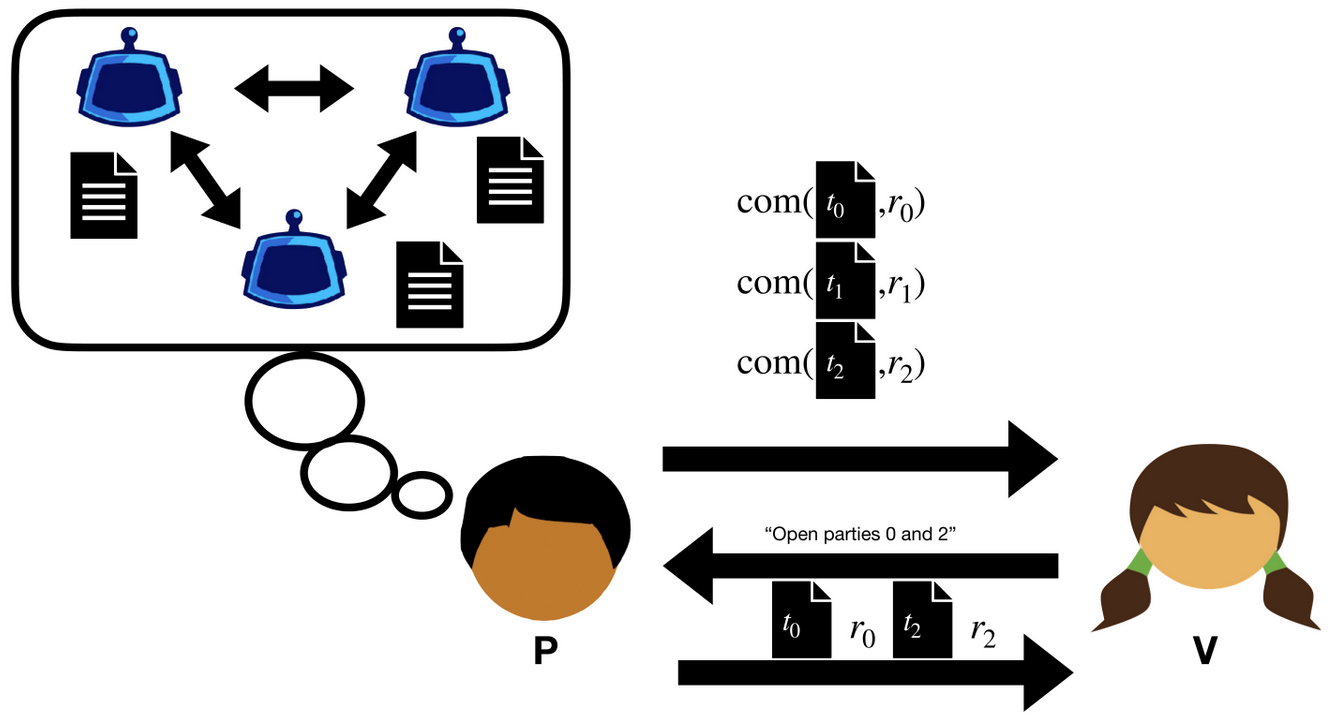
\includegraphics[width=0.7\textwidth]{figures/MPC-in-the-head.png}
  \caption{MPC-in-the-Head protocol.}
  \label{fig:mpcinthehead}
\end{figure}

The Ligero zk proof system does not require a trusted setup, and
is based on the following cryptographic assumptions:
\begin{itemize}
  \item \textbf{Collision-resistant hash functions}: Hash functions explained in section~\ref{cryptohashfunction};
  \item \textbf{Linear error-correcting codes}: Error-correcting codes are mathematical constructs that enable the 
  detection and correction of errors in data transmission or storage. They work by adding redundancy to the original data, 
  allowing the receiver to identify and correct errors without needing retransmission. In the context of Ligero, 
  linear error-correcting codes are used to ensure that even if some parts of the proof are tampered with or lost, 
  the verifier can still reconstruct the original information and verify its correctness;
  \item \textbf{Merkle trees}: Merkle trees are cryptographic data structures that consist of a binary tree of hash 
  values, where each leaf node represents a data block and each non-leaf node is the hash of its child nodes, as represented
  in image~\ref{fig:merkletree}. Merkle trees in Ligero are used to efficiently perform vector commitments;
\end{itemize}
All of these assumptions are quantum-resistant; therefore, Ligero is a post-quantum secure zero-knowledge proof system.

\begin{figure}
  \centering
  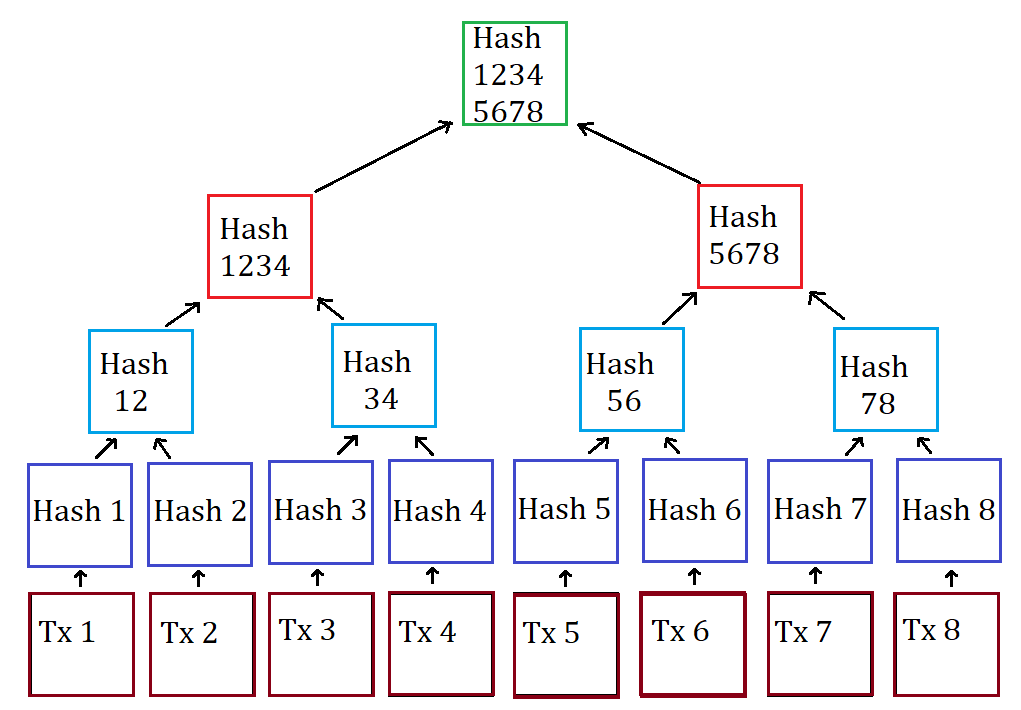
\includegraphics[width=0.7\textwidth]{figures/Merkle-tree.png}
  \caption{Merkle tree graphic representation.}
  \label{fig:merkletree}
\end{figure}

\paragraph{Protocol Workflow}
The following steps describe how a prover demonstrates knowledge of a valid witness for an arithmetic circuit of size $C$ over a finite field:
\begin{enumerate}
    \item \textbf{Matrix Layout:} The prover arranges the circuit's wire assignments into an $m \times n$ matrix, where $m, n \approx \sqrt{C}$.
    \item \textbf{Encoding and Commitment:} Each row is encoded via the linear code. The prover builds a Merkle tree over the columns of this extended matrix and sends the root to the verifier.
    \item \textbf{Linear Constraint Check:} The verifier sends random challenges to test if the linear and quadratic constraints of the circuit hold.
    \item \textbf{Proximity Testing:} The verifier samples random columns to ensure that the matrix rows are actually close to valid codewords.
\end{enumerate}

\paragraph{Asymptotic Efficiency and Trade-offs}
Ligero offers a favourable efficiency profile for a proof system with no trusted setup~\cite{Ames2017Ligero}:
\begin{itemize}
    \item \textbf{Proof Size:} $\mathcal{O}(\sqrt{|C|})$, which is a notable trade-off relative to the $\mathcal{O}(1)$ proof sizes of preprocessing SNARKs such as Groth16~\cite{cryptoeprint:2016/260}, but avoids the costly trusted setup phase entirely.
    \item \textbf{Prover Time:} $\mathcal{O}(|C|)$, making the prover linear in the circuit size and compatible with any sufficiently large finite field.
    \item \textbf{Verification Time:} $\mathcal{O}(\sqrt{|C|} \cdot \log |C|)$, sublinear in the circuit size and dominated by Merkle path verifications for the sampled columns.
\end{itemize}

\paragraph{Non-Interactive Variant}
The Ligero protocol as described above is interactive. 
In practice, the interactive challenges from the verifier are replaced by outputs of a cryptographic hash function modeled 
as a random oracle, following the Fiat-Shamir transform~\cite{FiatShamir1987}. This transformation yields a non-interactive 
argument of knowledge that preserves soundness and zero-knowledge in the random oracle model, and is the approach 
adopted in all practical Ligero implementations, including the one used in this work.

\subsection{STARK}
\label{STARK}
STARK is a zero-knowledge proof system proposed in 2018 by Ben-Sasson et al.~\cite{BenSasson2018STARK}.
The acronym stands for \emph{Scalable Transparent ARgument of Knowledge}.
STARKs are based on the following advanced cryptographic techniques:
\begin{itemize}
  \item \textbf{Algebraic Intermediate Representation (AIR)}~\cite{BenSasson2018STARK}: A computation of
  $n$ steps is encoded as an \emph{execution trace}, a matrix whose rows represent the register state at
  each step. Correctness of the computation is expressed as a set of polynomial constraints over the trace
  -- \emph{boundary constraints} that fix the initial and final states, and \emph{transition constraints}
  that assert consistency between consecutive rows. Proving the computation correct reduces to proving that
  these constraint polynomials vanish over the trace domain.
  \item \textbf{Fast Reed-Solomon IOP of Proximity (FRI)}~\cite{BenSasson2018FRI}: FRI is the core
  sub-protocol used to prove that a committed polynomial has bounded degree, without evaluating it
  everywhere. It works by recursively halving the polynomial's degree over $\mathcal{O}(\log n)$ rounds,
  each round producing a smaller commitment verified via Merkle tree. Random spot-checks by the verifier
  ensure that any cheating prover is caught with overwhelming probability.
\end{itemize}

The STARK proof system does not require a trusted setup, and is based on the following cryptographic
assumptions:
\begin{itemize}
  \item \textbf{Collision-resistant hash functions}: Hash functions explained in section~\ref{cryptohashfunction};
  \item \textbf{Merkle trees}: Merkle trees, as represented in figure~\ref{fig:merkletree}, are used throughout
  the STARK protocol as a vector commitment scheme, binding the prover to the execution trace and to each
  intermediate FRI oracle;
  \item \textbf{Reed-Solomon codes}: The low-degree extension of the execution trace over a larger evaluation
  domain encodes the witness as a Reed-Solomon codeword, and FRI proximity testing detects any deviation
  from a valid codeword.
\end{itemize}
All of these assumptions are quantum-resistant; therefore, STARK is a post-quantum secure zero-knowledge
proof system.

\paragraph{Protocol Workflow}
The following steps describe how a prover demonstrates that a computation of length $n$ was carried out correctly:
\begin{enumerate}
  \item \textbf{Trace Commitment:} The prover builds the execution trace matrix and evaluates each column
  polynomial over a larger domain (low-degree extension). The extended evaluations are committed via a Merkle tree.
  \item \textbf{Constraint Composition:} The verifier sends random challenges; the prover combines all
  constraint polynomials into a single composition polynomial and commits to it with a second Merkle tree.
  \item \textbf{FRI Protocol:} The prover runs FRI on the composition polynomial to prove its degree is
  within the expected bound, sending one Merkle root per folding round.
  \item \textbf{Query Phase:} The verifier samples random positions; the prover opens the trace, composition,
  and all FRI oracles at those positions with Merkle authentication paths.
\end{enumerate}

\paragraph{Asymptotic Efficiency and Trade-offs}
STARKs achieve the following asymptotic complexities~\cite{BenSasson2018STARK}:
\begin{itemize}
  \item \textbf{Proof Size:} $\mathcal{O}(\log^2 n)$, poly-logarithmic in the trace length, which is
  significantly smaller than Ligero's $\mathcal{O}(\sqrt{n})$ for large computations.
  \item \textbf{Prover Time:} $\mathcal{O}(n \log n)$, quasi-linear, dominated by the FFTs needed for the
  low-degree extension and FRI folding rounds.
  \item \textbf{Verification Time:} $\mathcal{O}(\log^2 n)$, dominated by the Merkle path verifications
  across the FRI rounds.
\end{itemize}

\paragraph{Non-Interactive Variant}
The STARK protocol as described above is interactive.
In practice, the interactive challenges from the verifier are replaced by outputs of a cryptographic hash
function modeled as a random oracle, following the Fiat-Shamir transform~\cite{FiatShamir1987}. This
transformation yields a non-interactive argument of knowledge that is the standard form used in all
practical STARK libraries, including Winterfell~\cite{FacebookWinterfell}, which is the backend adopted
in this work.



\chapter{EUropean Digital Identity Wallet}
\label{eudiw}
In 2021, the European Commission proposed to adopt a framework for a European Digital Identity~\cite{EuropeanCommission2021EUDI}.
In 2024, the European Commission decided to establish an Architecture Reference Framework (ARF)~\cite{EuropeanCommission2024EUDIARF},
which consisted of a set of guidelines and properties that each instance of the wallet application should satisfy.
This general framework is needed since the commission left freedom to each member state to implement their own 
instance of the application, due to different possible credentials structures (for example, French and German national 
identity cards have different structures and/or attributes) and infrastructures (for example, some member states have 
already a national identity card with an embedded chip, while others don't).

In the following section, we are going to analyze the architecture of the EUDI wallet application,to give a complete 
overview of Architecture Reference Framework, and to analyze the vulnerabilities of the proposed implementation.

\section{Cryptographic Foundations}
\label{eudi:crypto}
The entire ecosystem is built on a \textbf{Public Key Infrastructure (PKI)}. The main primitives and standards are the
following:
\begin{itemize}[noitemsep]
  \item \textbf{Elliptic-Curve Cryptography (ECC)} is the preferred choice for mobile-device performance. The relevant
        presentation standards, ISO/IEC~18013-5~\cite{iso18013-5} and SD-JWT~VC~\cite{sdjwtvc}, rely respectively on the
        \textbf{COSE} (CBOR Object Signing and Encryption) and \textbf{JOSE} (JSON Object Signing and Encryption)
        frameworks.
  \item \textbf{RSA} is also supported, together with \textbf{X.509} certificates~\cite{rfc5280} and the ETSI standards
        used for qualified electronic signatures.
\end{itemize}
For signing documents and transactions the ARF explicitly references the ETSI \emph{AdES} (Advanced Electronic
Signature) profiles, namely \textbf{XAdES}, \textbf{PAdES}, \textbf{CAdES} and \textbf{JAdES}, depending on the data
format being signed.

It is important to stress already at this point that, although the PKI is format-agnostic in principle, the
\emph{device-binding} keys -- the keys that anchor a credential to a specific device -- must reside in the device's
secure hardware, which in practice today only supports ECDSA over the NIST P-256 curve. This constraint is central to
our solution, discussed in \cref{oursolution}.

\section{Functionalities}
\label{eudi:functionalities}
At a high level, the functionalities offered by a Wallet Unit can be grouped into four categories:
\begin{itemize}[noitemsep]
  \item \textbf{Secure identification and authentication}, ensuring that users can present person identification data
        (PID) in a trusted environment, both online and in proximity.
  \item \textbf{Exchanging qualified and non-qualified user attributes} through secure and verifiable electronic
        attestations of attributes (EAAs).
  \item \textbf{Electronic signing of documents or data}, allowing users to create legally recognised qualified
        electronic signatures and seals.
  \item \textbf{Generation and use of pseudonyms} for authentication, to enhance privacy and prevent tracking.
\end{itemize}
A further, emerging use case is the wallet acting as a \emph{strong customer authentication} device for payments,
discussed in \cref{eudi:payments}.

Now we will discuss in depth each of these functionalities, describing the involved actors and the protocols used to implement them.

\subsection{Identification and Authentication}
\label{eudi:auth}
\textbf{Description.} Users can identify and authenticate to online and offline services while using
\emph{selective disclosure} of attributes or attestations.

\textbf{Actors.} User; Wallet Unit (a smartphone application); Relying Party (the service requesting data); PID Provider.

\textbf{Protocols.} Two complementary protocols are used:
\begin{itemize}[noitemsep]
  \item \textbf{ISO/IEC~18013-5}~\cite{iso18013-5} for \emph{proximity} flows. The Wallet Unit and the Relying Party set
        up a communication channel using a QR code or NFC and then communicate over BLE, NFC or Wi-Fi Aware. The standard
        provides confidentiality and authenticity for all exchanged data, as well as Relying Party authentication.
        \Cref{fig:proximity} sketches the proximity flow.
  \item \textbf{OpenID4VP}~\cite{openid4vp} for \emph{remote} (including cross-device) flows. It defines the message
        structures, transaction flows and an HTTP-based interface for presenting attestations from a Wallet Unit to a
        Relying Party, again providing confidentiality, authenticity and Relying Party authentication.
        \Cref{fig:remote} sketches the remote, cross-device flow.
\end{itemize}

\begin{figure}[ht]
  \centering
  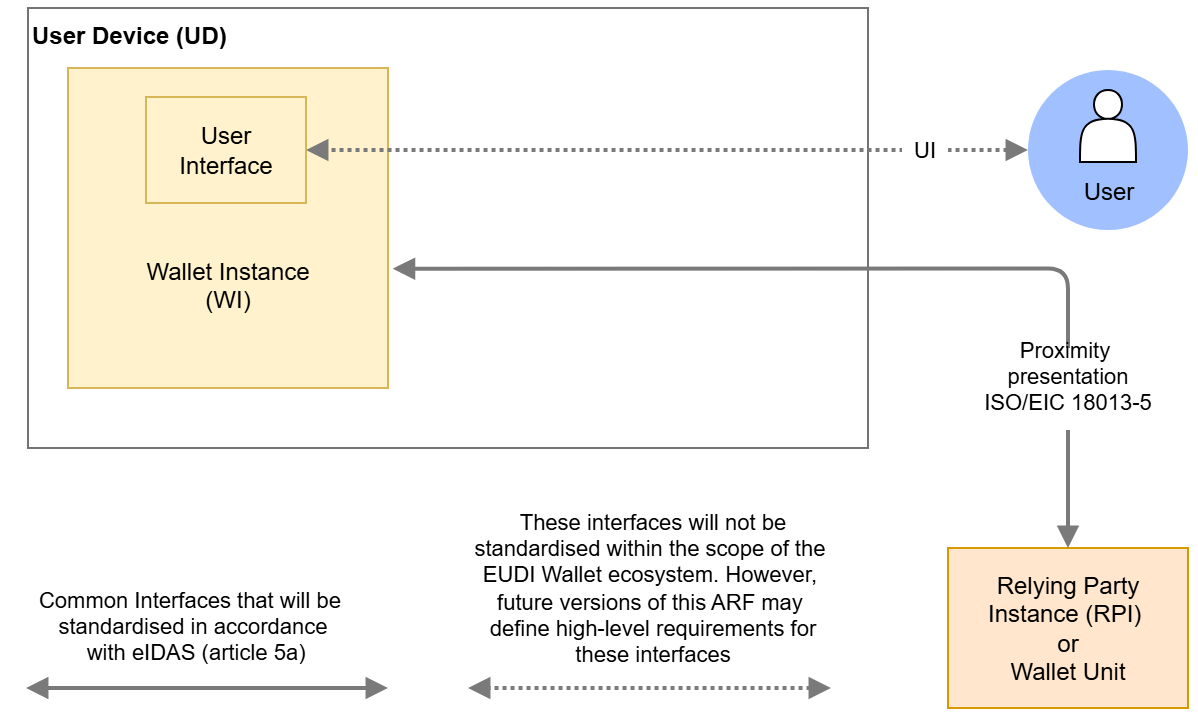
\includegraphics[width=0.85\textwidth]{figures/Figure_3_Proximity_Flow.png}
  \caption{Proximity presentation flow (ISO/IEC 18013-5). Adapted from the ARF~\cite{EuropeanCommission2024EUDIARF}.}
  \label{fig:proximity}
\end{figure}

\begin{figure}[ht]
  \centering
  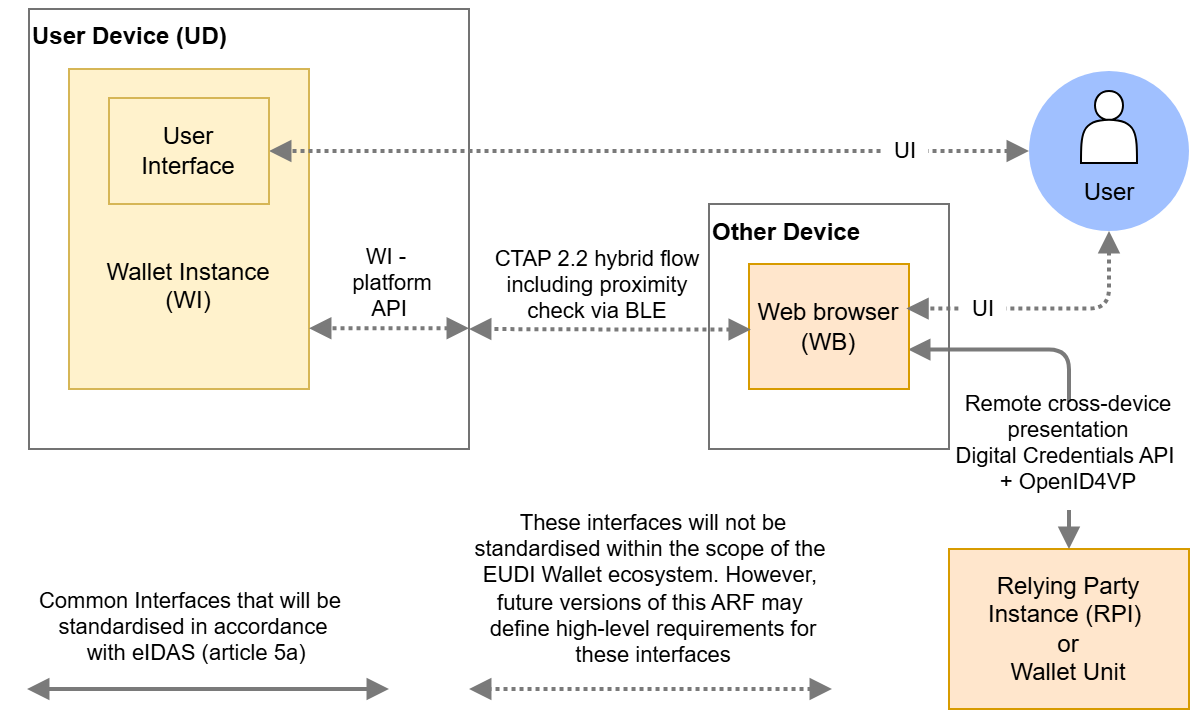
\includegraphics[width=0.85\textwidth]{figures/Figure_5_Remote_Cross-Device_Flow.png}
  \caption{Remote, cross-device presentation flow (OpenID4VP). Adapted from the ARF~\cite{EuropeanCommission2024EUDIARF}.}
  \label{fig:remote}
\end{figure}

In both protocols, \textbf{device binding} is achieved by including a cryptographic public key in the PID or attestation
and signing it; the corresponding private key is protected by a Wallet Secure Cryptographic Application/Device
(WSCA/WSCD) or keystore inside the Wallet Unit. Although the proximity and remote protocols differ in their details, at a
high level they both implement \textbf{Relying Party authentication} as illustrated in \cref{fig:rpauth}.

\begin{figure}[ht]
  \centering
  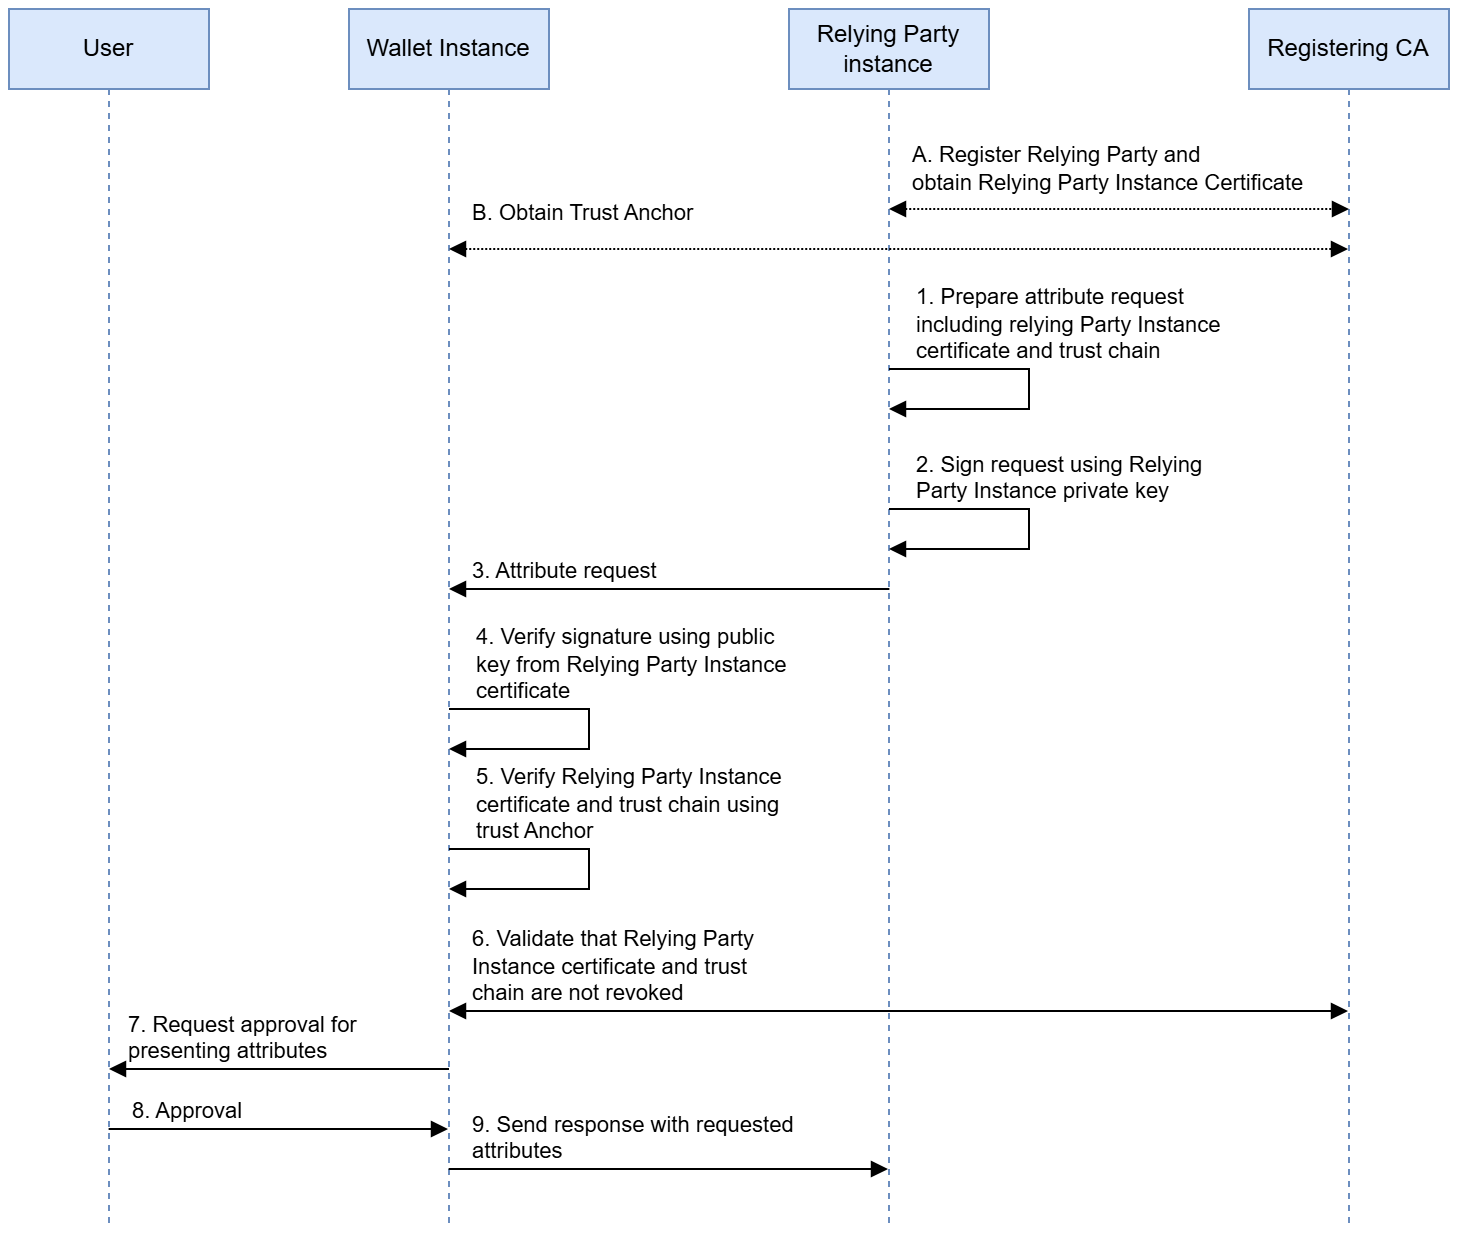
\includegraphics[width=0.8\textwidth]{figures/Figure_13_Relying_Party_Authentication.png}
  \caption{Relying Party authentication, common to the proximity and remote flows. Adapted from the ARF~\cite{EuropeanCommission2024EUDIARF}.}
  \label{fig:rpauth}
\end{figure}

\subsection{Exchanging User Attributes}
\label{eudi:attributes}
\textbf{Description.} The wallet lets a user request, store and share Electronic Attestations of Attributes -- EAA,
PuB-EAA and QEAA. The wallet supports \emph{selective disclosure}, so that the user can share only a subset of the
attributes contained in an attestation.

\textbf{Actors.} User; Wallet Unit; Relying Party; Attestation Provider (QEAA, PuB-EAA or EAA), the entity issuing the
attestation.

\textbf{Protocol.} \emph{SD-JWT~VC}~\cite{sdjwtvc} (Selectively Disclosable JSON Web Token Verifiable Credentials) is a
special form of JWT that is selectively disclosable. It specifies the JSON encoding of attributes and metadata together
with rules that prevent collisions of claim names; a proof mechanism that ensures the authenticity and integrity of a
PID or attestation while allowing selective disclosure of individual attributes; and an \emph{optional} security
mechanism enabling device binding of PIDs and attestations. \Cref{fig:sdjwt} illustrates the structure of an
SD-JWT~VC.

\begin{figure}[ht]
  \centering
  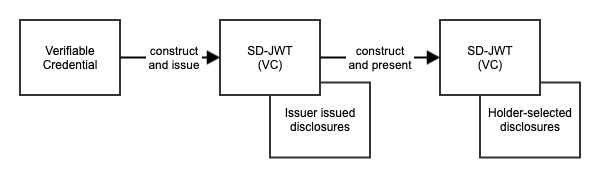
\includegraphics[width=0.85\textwidth]{figures/SD-JWT-VC.png}
  \caption{Structure and selective-disclosure mechanism of an SD-JWT VC. Adapted from the SD-JWT VC specification~\cite{sdjwtvc}.}
  \label{fig:sdjwt}
\end{figure}

\paragraph{How attestations are added.} For mobile driving licenses (mDL) the Attestation Rulebook explicitly references
the ISO/IEC~18013-5 model, the same used for identification. Other attestations are obtained as follows: the user first
verifies that the provider is trusted (it appears on an official Trusted List or List of Trusted Entities); the provider
authenticates the user, typically reusing the OpenID4VP authentication flow; the provider validates the Wallet Instance
through its Wallet Instance Attestation; the user reviews and approves the attestation; and finally the wallet verifies
the provider's signature on the attestation and stores it.

\paragraph{How attestations are stored.} The ARF mandates a small set of standardised formats:
\begin{itemize}[noitemsep]
  \item \textbf{CBOR}, used by ISO/IEC~18013-5. It is mandatory for mDLs and may be used for any other attestation if the
        provider remains compliant with the standard.
  \item \textbf{JWT}, used by SD-JWT~VC. No credential is required to be expressed in this format, but wallet support is
        mandatory.
  \item \textbf{W3C Verifiable Credentials Data Model v2.0}~\cite{w3cvcdm}, an optional format valid only for
        non-qualified EAAs and still under development.
\end{itemize}
\Cref{tab:formats} summarizes the three formats and their proof mechanisms.

\begin{table}[ht]
  \centering
  \caption{Attestation formats and proof mechanisms supported by the ARF.}
  \label{tab:formats}
  \small
  \begin{tabularx}{\textwidth}{@{}l L L L@{}}
    \toprule
    \textbf{Feature} & \textbf{ISO/IEC 18013-5 / 23220-2} & \textbf{SD-JWT VC} & \textbf{W3C VCDM v2.0} \\
    \midrule
    Data format    & CBOR (binary)            & JSON Web Token (JSON)        & JSON-LD (linked data) \\
    Proof type     & Embedded (salted hashes) & Embedded (salted hashes)     & Detached or embedded \\
    Key use case   & Proximity (e.g.\ mDL)    & Remote (e.g.\ remote ident.) & General (requires profiling) \\
    Wallet support & Mandatory                & Mandatory                    & Optional \\
    \bottomrule
  \end{tabularx}
\end{table}

\paragraph{How selective disclosure works.} Both ISO/IEC~18013-5 and SD-JWT~VC realize selective disclosure through the
\emph{salted-hash} technique combined with device and user binding:
\begin{itemize}[noitemsep]
  \item \textbf{Salted hashes.} The issuer signs a token in which each attribute is replaced by a salted hash of its
        value rather than its clear text (e.g.\ the hash of \texttt{family\_name:\,Rossi} together with a random salt).
        To disclose an attribute, the user reveals the clear value and the salt; the verifier recomputes the hash and
        checks that it matches the one inside the signed token.
  \item \textbf{Device binding.} The attestation embeds a public key whose private counterpart never leaves the WSCD.
        The provider/verifier issues a random challenge that the device signs, proving that it holds the private key
        bound to the attestation.
  \item \textbf{User binding.} Before disclosure, the wallet shows the user which attributes are about to be sent and
        requires local authentication (PIN, biometrics, etc.).
\end{itemize}
Zero-knowledge proofs, which would allow attributes to be proven without revealing the underlying field, are not yet
part of the supported mechanisms; their status is discussed later in the analysis.

\subsection{Qualified Electronic Signatures (QES)}
\label{eudi:qes}
\textbf{Description.} The wallet lets users create legally recognised qualified electronic signatures and seals for
legally binding transactions and document signing.

\textbf{Actors.} User; Wallet Unit; a \emph{local QSCD} (a local tamper-resistant device that produces signatures) or a
remote \emph{QESRC} provider (Qualified Electronic Signature Remote Creation).

\textbf{Protocol.} Communication between the Wallet Unit and the QSCD/WSCD takes place through a \emph{Secure
Cryptographic Interface}. All parties in the ecosystem that handle cryptographic keys -- Wallet Providers, PID and
Attestation Providers, Trusted List/LoTE Providers, Providers of Registration Certificates and Access Certificate
Authorities -- typically rely on a certified \textbf{Hardware Security Module (HSM)} to generate and manage private and
secret keys. In other words, the security of this functionality rests almost entirely on \emph{hardware} components,
which perform key generation and management, user authentication, and the production of signatures and seals; the choice
of the actual key-generation protocol is delegated to the wallet implementer.

\subsection{Pseudonyms}
\label{eudi:pseudonyms}
\textbf{Description.} Users can present a pseudonym to a Relying Party in situations where the Relying Party does not need
to learn the user's identity, which helps users avoid being tracked across services.

\textbf{Actors.} User; Wallet Unit; Relying Parties.

\textbf{Protocol.} The ARF distinguishes three kinds of pseudonyms:
\begin{itemize}[noitemsep]
  \item \emph{Verifiable} pseudonyms, which let the user prove ownership;
  \item \emph{Attested} pseudonyms, a sub-type of verifiable pseudonyms in which a third party attests that the pseudonym
        belongs to the user;
  \item \emph{Scope rate-limited} pseudonyms, a sub-type that guarantees the user controls at most a fixed number (the
        \emph{rate}) of pseudonyms for a given scope.
\end{itemize}
\textbf{W3C WebAuthn}~\cite{webauthn} specifies a class of verifiable pseudonyms known as \emph{passkeys}. The protocol
has two phases:
\begin{enumerate}[noitemsep]
  \item \textbf{Registration.} The user generates a public/private key pair, stores both keys in a secure device (the
        \emph{Authenticator}), and registers the public key with the desired Relying Party.
  \item \textbf{Authentication.} When the user wishes to authenticate, the service sends a challenge consisting of a
        random value; the user signs it with the private key held by the Authenticator and returns the signature; the
        service verifies the signature against the registered public key and, if the signature and the origin match,
        grants access.
\end{enumerate}
Pseudonyms are stored encrypted in a local secure area of the device. \Cref{fig:webauthn} illustrates the WebAuthn
authentication scheme.

\begin{figure}[ht]
  \centering
  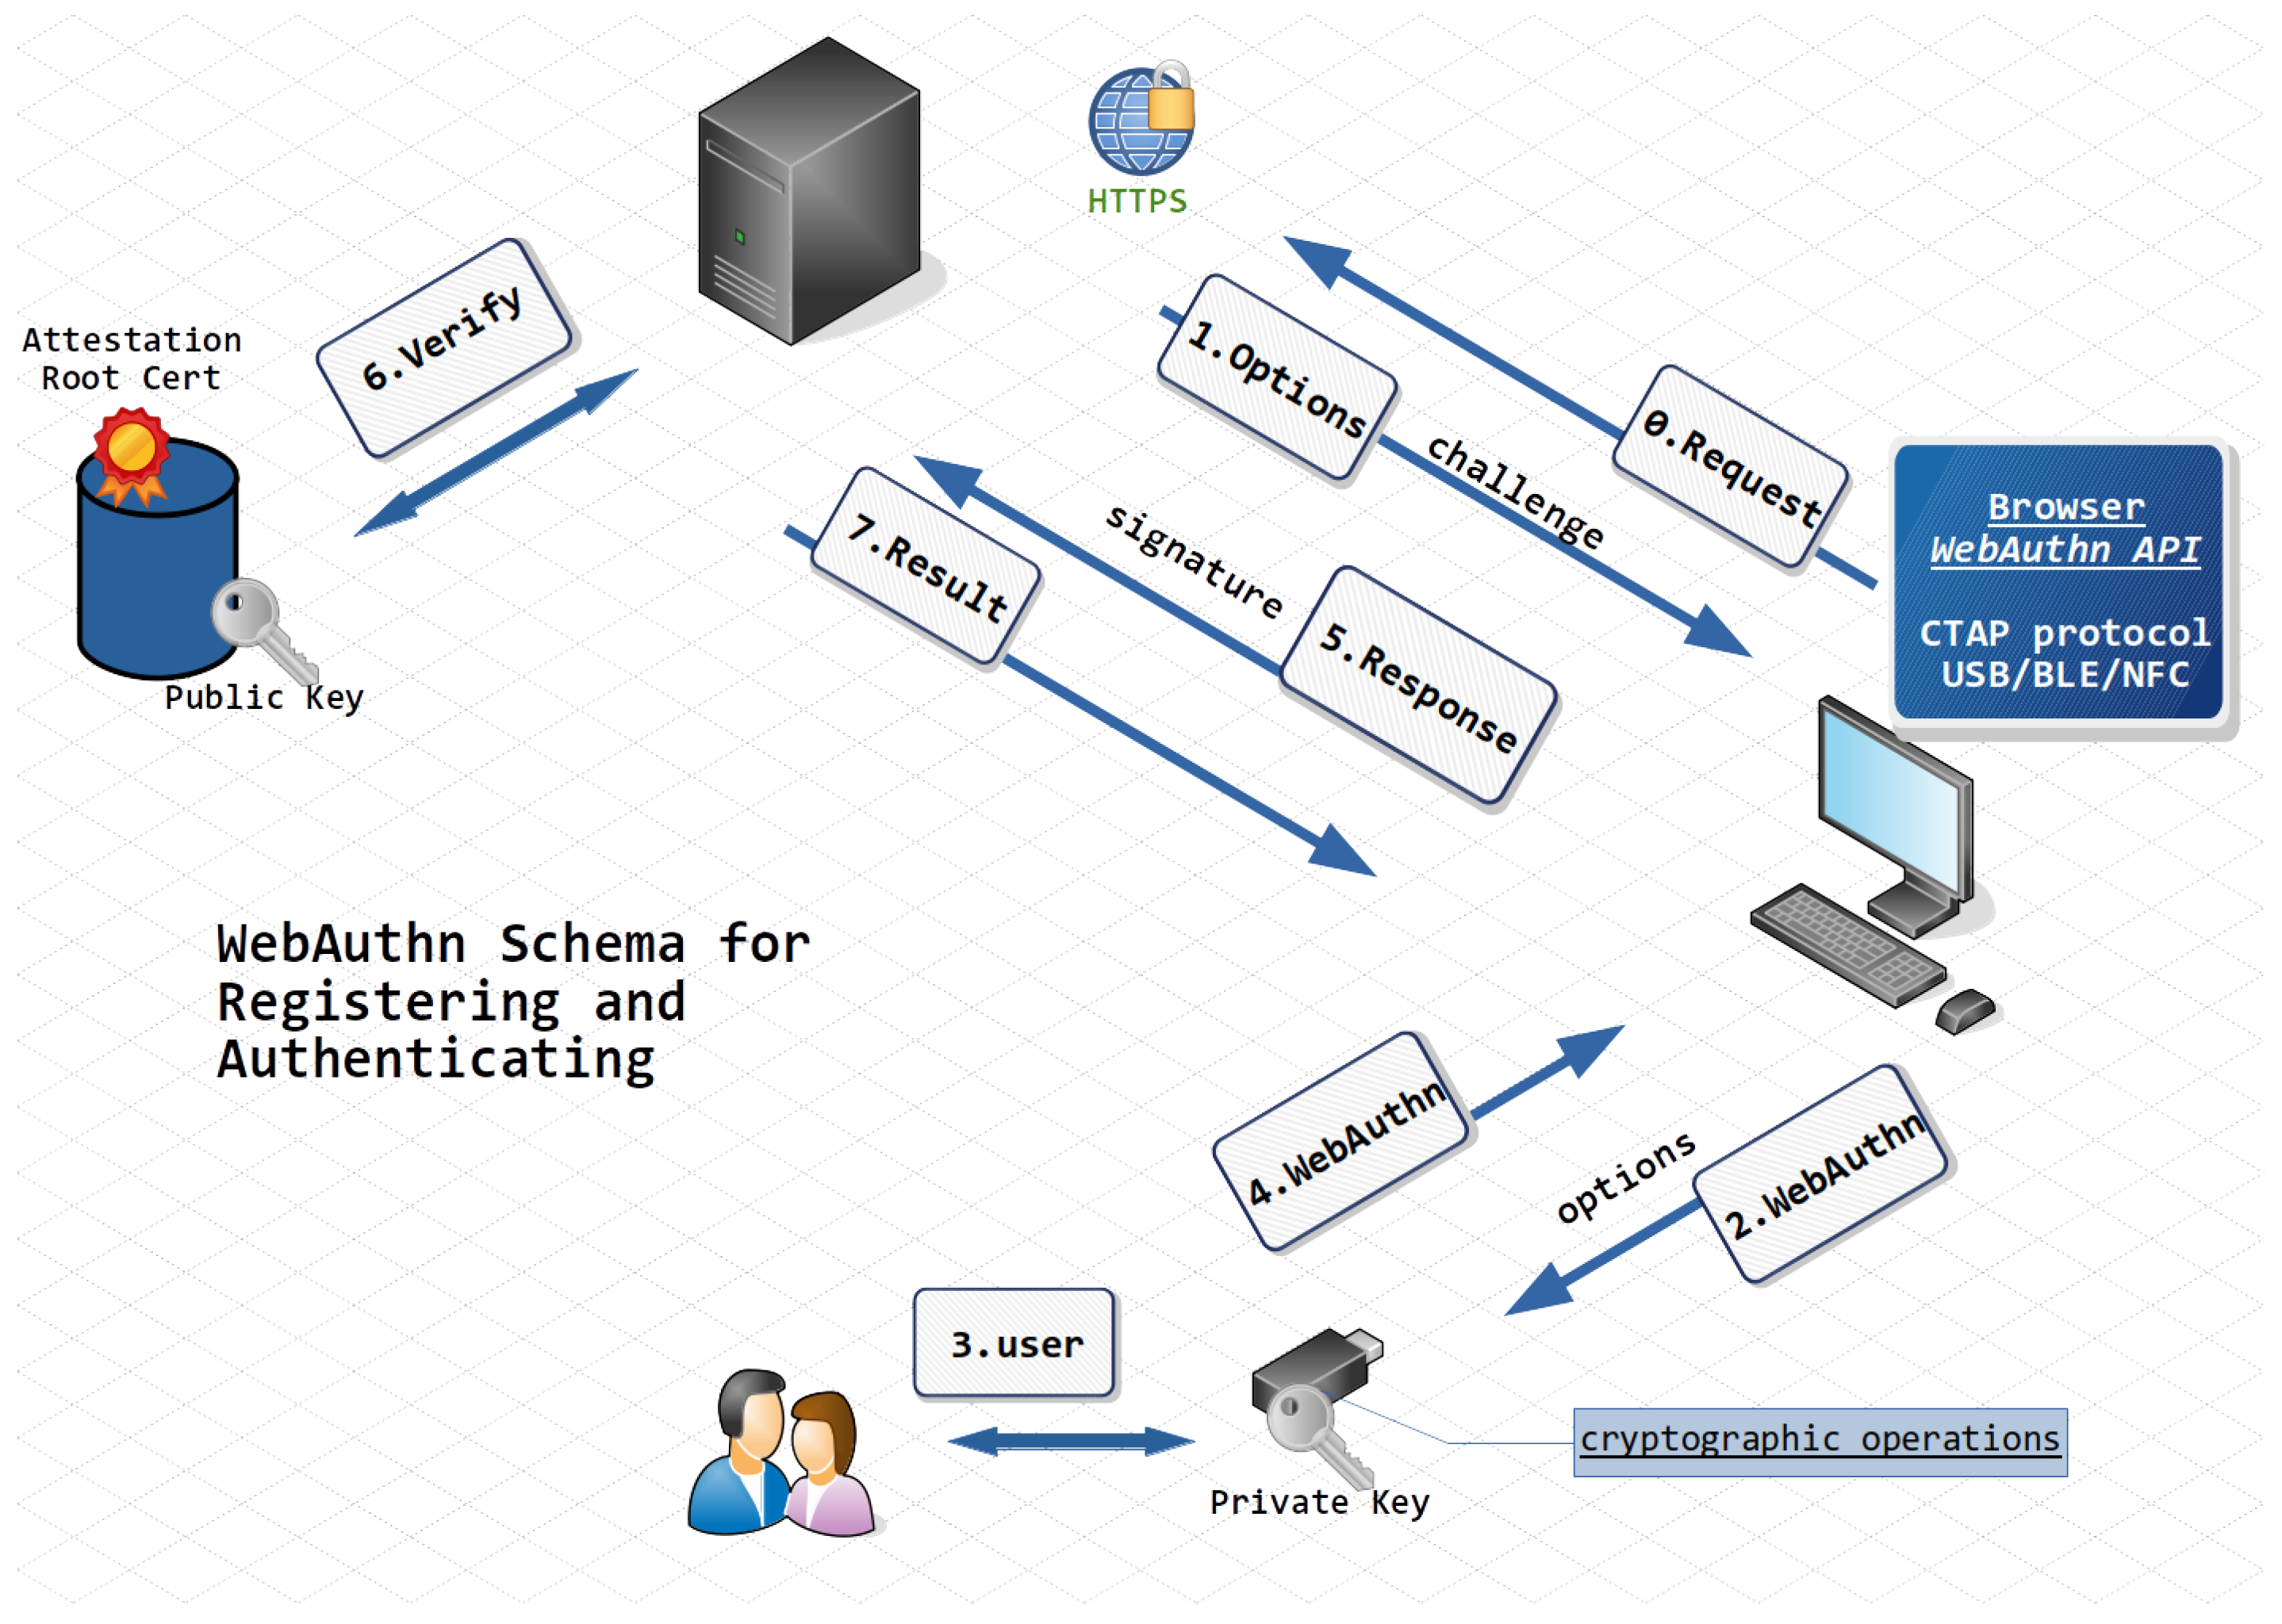
\includegraphics[width=0.8\textwidth]{figures/webauthn.png}
  \caption{W3C WebAuthn authentication scheme used for verifiable pseudonyms (passkeys). Adapted from~\cite{webauthn}.}
  \label{fig:webauthn}
\end{figure}

\subsection{Payments}
\label{eudi:payments}
The EUDI Wallet acts as an \emph{authenticator} that lets the user authorise payments. Unlike, for example, Google
Wallet -- which typically stores a tokenized version of a physical card -- the EUDI Wallet does not store a card number.
Instead, it is issued a \textbf{Strong User Authentication (SUA)} attestation: a verified digital document that links the
Wallet Unit to a specific bank account or payment service. This SUA attestation is \emph{device-bound}, i.e.\
cryptographically tied to the secure hardware (WSCD/WSCA) of the user's phone.

When a payment is made, the merchant (acting as a Relying Party) sends the wallet a request containing the transactional
data. The user reviews the request on screen and, upon consent, the wallet signs that specific data with its internal
keys to authorise the payment. The process is designed to satisfy the \textbf{Strong Customer Authentication (SCA)}
requirements of the EU payment-services framework (PSD2/PSD3)~\cite{psd2}. The payment life cycle therefore has three
phases: \emph{registration} (linking the wallet to the bank via an SUA attestation), \emph{authentication} (approving a
transaction by signing the amount and payee) and \emph{termination} (unlinking by revoking the SUA attestation).

\section{Roles}
\label{roles}

\begin{figure}[H]
  \centering
  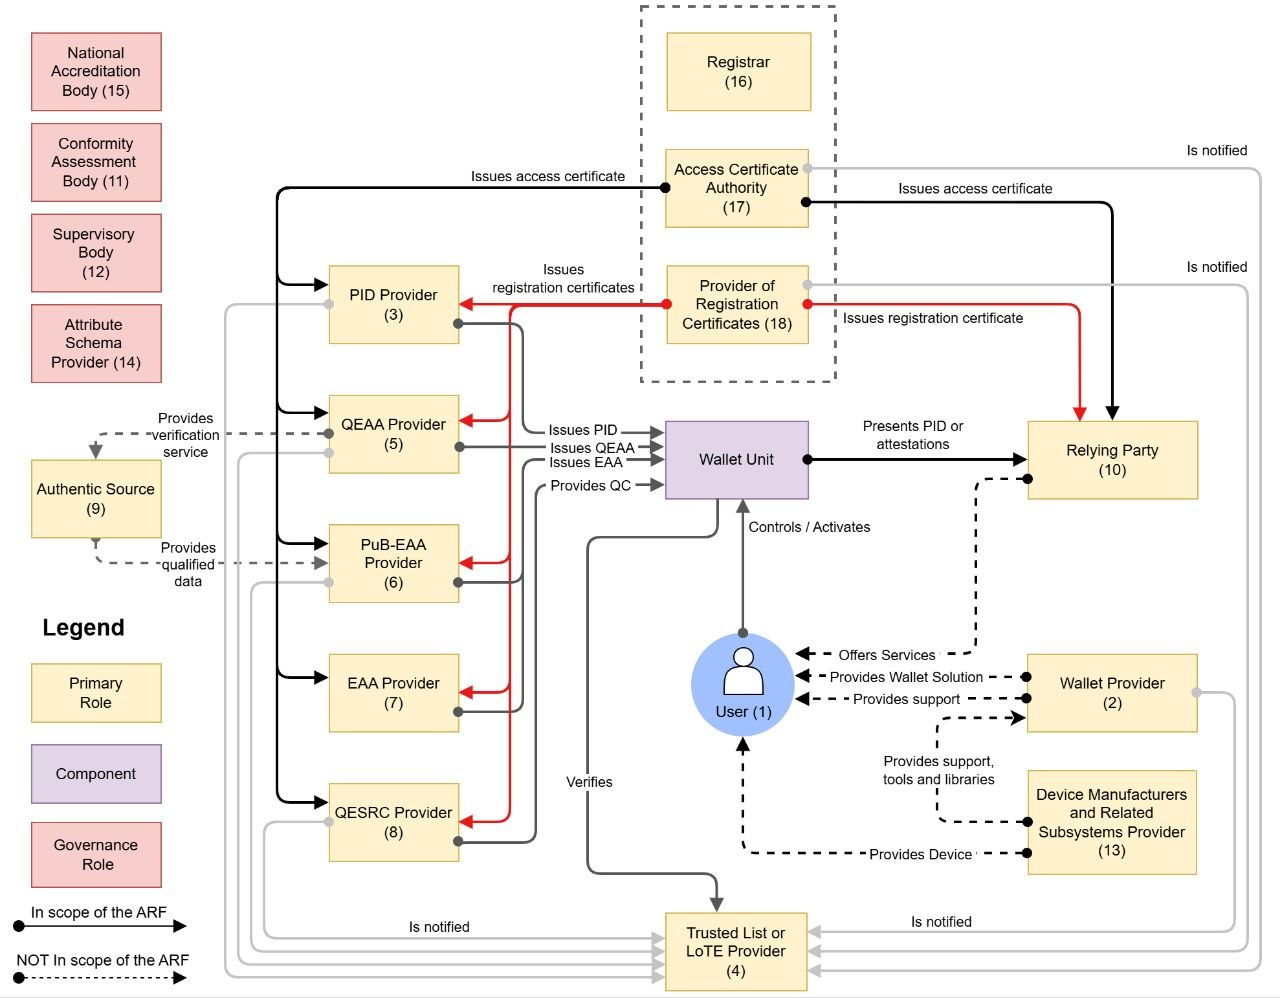
\includegraphics[width=0.6\textwidth]{figures/Pasted image 20260224155454.png}
  \caption{EUDI Architecture Reference Framework roles and responsibilities. Adapted from~\cite{EuropeanCommission2024EUDIARF}.}
  \label{fig:arfroles}
\end{figure}

\begin{table}[htbp]
    \centering
    \caption{Roles and Responsibilities within the EUDI Wallet Ecosystem}
    \label{tab:roles}
    \small
    \begin{tabularx}{\textwidth}{@{}l L l@{}}
        \toprule
        \textbf{Role} & \textbf{Primary Responsibility} & \textbf{Section} \\
        \midrule
        \textbf{User of Wallet Unit} & Manage, store, and present PIDs/attestations. & \href{https://eudi.dev/latest/architecture-and-reference-framework-main/\#32-users-of-wallet-units}{ARF Section 3.2} \\
        \textbf{Wallet Provider} & Make the certified Wallet Solution available to Users. & \href{https://eudi.dev/latest/architecture-and-reference-framework-main/\#33-wallet-providers}{ARF Section 3.3} \\
        \textbf{PID Provider} & Issue Person Identification Data (PID) to Users. & \href{https://eudi.dev/latest/architecture-and-reference-framework-main/\#34-person-identification-data-pid-providers}{ARF Section 3.4} \\
        \textbf{Trusted List/LoTE Provider} & Maintain, manage, and publish Trusted Lists and/or Lists of Trusted Entities. & \href{https://eudi.dev/latest/architecture-and-reference-framework-main/\#35-trusted-list-or-lote-provider}{ARF Section 3.5} \\
        \textbf{QEAA Provider} & Issue Qualified Electronic Attestations of Attributes (QEAAs). & \href{https://eudi.dev/latest/architecture-and-reference-framework-main/\#36-qualified-electronic-attestation-of-attributes-qeaa-providers}{ARF Section 3.6} \\
        \textbf{PuB-EAA Provider} & Issue EAAs on behalf of a public sector body. & \href{https://eudi.dev/latest/architecture-and-reference-framework-main/\#37-eaa-issued-by-or-on-behalf-of-a-public-sector-body-responsible-for-an-authentic-source-pub-eaa-providers}{ARF Section 3.7} \\
        \textbf{EAA Provider} & Issue Non-Qualified Electronic Attestations of Attributes (EAAs). & \href{https://eudi.dev/latest/architecture-and-reference-framework-main/\#38-non-qualified-electronic-attestation-of-attributes-eaa-providers}{ARF Section 3.8} \\
        \textbf{QESRC Provider} & Provide Qualified Electronic Signature Remote Creation services. & \href{https://eudi.dev/latest/architecture-and-reference-framework-main/\#39-qualified-electronic-signature-remote-creation-qesrc-providers}{ARF Section 3.9} \\
        \textbf{Authentic Source} & Act as the definitive repository for specific attributes. & \href{https://eudi.dev/latest/architecture-and-reference-framework-main/\#310-authentic-sources}{ARF Section 3.10} \\
        \textbf{Relying Party (RP)} & Request and receive attributes from a Wallet Unit. & \href{https://eudi.dev/latest/architecture-and-reference-framework-main/\#311-relying-parties-relying-party-instances-and-intermediaries}{ARF Section 3.11} \\
        \textbf{CAB} & Certify Wallet Solutions and audit Trust Service Providers. & \href{https://eudi.dev/latest/architecture-and-reference-framework-main/\#312-conformity-assessment-bodies-cab}{ARF Section 3.12} \\
        \textbf{Supervisory Body} & Review the proper functioning of ecosystem actors. & \href{https://eudi.dev/latest/architecture-and-reference-framework-main/\#313-supervisory-bodies}{ARF Section 3.13} \\
        \textbf{Device Manufacturers} & Provide the underlying platform (hardware, OS, secure elements). & \href{https://eudi.dev/latest/architecture-and-reference-framework-main/\#314-device-manufacturers-and-related-subsystems-providers}{ARF Section 3.14} \\
        \textbf{Attestation Scheme Provider} & Define and publish the Attestation Rulebooks and schemes. & \href{https://eudi.dev/latest/architecture-and-reference-framework-main/\#315-attestation-scheme-providers-for-qeaas-pub-eaas-and-eaas}{ARF Section 3.15} \\
        \textbf{NAB} & Accredit CABs according to EU regulations. & \href{https://eudi.dev/latest/architecture-and-reference-framework-main/\#316-national-accreditation-bodies}{ARF Section 3.16} \\
        \textbf{Registrar} & Manages the registration of Providers and Relying Parties. & \href{https://eudi.dev/latest/architecture-and-reference-framework-main/\#317-registrars}{ARF Section 3.17} \\
        \textbf{Access CA} & Issue access certificates for authentication. & \href{https://eudi.dev/latest/architecture-and-reference-framework-main/\#318-access-certificate-authorities}{ARF Section 3.18} \\
        \textbf{Provider of Reg. Certs} & Issue certificates detailing registration status and scope. & \href{https://eudi.dev/latest/architecture-and-reference-framework-main/\#319-providers-of-registration-certificates}{ARF Section 3.19} \\
        \bottomrule
    \end{tabularx}
\end{table}

\clearpage

\section{The Concept of Level of Assurance (LoA) High}
\label{loa}
In the context of the eIDAS 2.0 framework and digital identity systems, the Level of Assurance (LoA) represents the degree 
of confidence in the claimed identity of a person. It is a critical metric used to determine how much a Relying Party can trust
that the user presenting a credential is indeed the person they claim to be.

The technical specifications and procedures for these levels are strictly regulated by Commission Implementing Regulation (EU) 
2015/1502.
\subsection{Definition of LoA High}
The LoA High is the highest tier of security defined under the eIDAS regulation. It is designed to protect against attackers
with a high attack potential. According to the standard, a "High" level provides a near-absolute degree of certainty in the 
identity of the user, making it mandatory for sensitive operations such as accessing critical government services or opening 
financial accounts.

\subsection{Key Security Requirements}
To achieve a High Level of Assurance, several technical and organizational criteria must be met:
\begin{itemize}
      \item \textbf{Secure Cryptographic Hardware:} The cryptographic keys (specifically those associated with the Person Identification Data or PID) must be managed within a Wallet Secure Cryptographic Device (WSCD). This device is legally required to comply with the requirements of LoA High, ensuring that keys are protected against unauthorized duplication or tampering.
      \item \textbf{Common Criteria Certification:} A core determinant for LoA High is the certification of the secure element. It must typically reach a Common Criteria (CC) evaluation level of AVA\_VAN.5. This specific level certifies that the device can resist sophisticated, state-level attacks performed by highly capable adversaries.
      \item \textbf{Dynamic Authentication:} The authentication process must be dynamic, meaning the proof generated by the wallet must change for every session. This prevents replay attacks, where an intercepted proof could be used by an unauthorized party.
      \item \textbf{Multi-Factor Authentication (MFA):} LoA High requires the use of at least two authentication factors from different categories, such as "possession" (the device) and "inherence" (biometrics like fingerprints or facial recognition).
\end{itemize}

\subsection{LoA High in the EUDI Wallet Ecosystem}
Within the EUDI Wallet, the PID is the only attestation that is strictly required by regulation to be issued and managed at LoA High. While other Electronic Attestations of Attributes (EAAs) may use lower levels, the infrastructure of the Wallet must support the High tier to ensure the integrity of the user's core identity. The transition to post-quantum-safe Zero-Knowledge Proofs (ZKPs) is also being explored as a method to maintain this high level of assurance in a future where quantum computers could threaten classical ECC-based security.

\section{Zero-knowledge Proofs in the ARF}
\label{eudi:zkp}
Citing ARF developer guide at section \href{https://eudi.dev/latest/architecture-and-reference-framework-main/#74353-zero-knowledge-proofs}{7.4.3.5.3 Zero-knowledge proofs},
Unlike Relying Party linkability, attestation Provider linkability cannot be fully eliminated when using attestation formats based on salted hashes. The only viable mitigation, they say,
is to adopt Zero-Knowledge Proofs (ZKPs) as a verification mechanism instead of relying on salted-attribute hashes.

Furthermore, navigating the ARF developers guide, we found the following statements:
Zero-Knowledge Proof (ZKP) mechanisms for verifying personal information are highly promising and essential for ensuring privacy in various use cases. They enable Users to prove 
statements such as "I am over 18" without disclosing any personal data, offering a robust solution for privacy-preserving authentication and verification.

However, the integration of ZKPs in the EUDI Wallet ecosystem is still under discussion and development, due to the complexity of implementing ZKP solutions in secure hardware and the 
lack of support in currently available secure hardware (WSCDs). As with Relying Party linkability, organizational and enforcement measures can help deter Attestation Providers from 
colluding and tracking Users. Additionally, many Attestation Providers are subject to regular audits, making it easier to detect collusion and tracking compared to Relying Parties.

% Ecc...
\section{Vulnerabilities}
\label{vulnerabilities}
In this section we are going to analyze the main vulnerabilities of the EUDI wallet found by us, and
known in the scientific community.

\paragraph{Linkability}
Presentations are signed with (and reveal) PKu; PKu and EAArevoc\_id persist
across sessions; salted hashes stay constant across presentations. Misactors
(RPs, APs, WPs, supervisory bodies, external) can correlate repeat
interactions and link them to attributable data.

\paragraph{Information leakage through salted-hash selective disclosure}
Proving a predicate such as "Age over 18" with salted hashes forces disclosure 
of the WHOLE field, i.e. the full date of birth. 
Likewise proving nationality may leak the full address / city of
residence. The selective-disclosure mechanism lacks granularity: it can only
reveal or hide a whole attribute, never a derived predicate.
Note on the proposed mitigation: the spec suggests the issuer pre-bakes
boolean fields (e.g. "adult: yes/no"). This mitigation is clearly unworkable: 
it does not scale to arbitrary thresholds (over 19, over 20, ...).

\paragraph{No backup/recovery mechanism}
The system provides no backup/recovery. If the wallet device is
lost, the user loses access to all his credentials, pseudonyms ecc. 
Moreover, if the device gets broken, Keys are trapped inside the 
Secure Element and cannot be moved out (QESRC keys cannot leave the SE).

\paragraph{Secure element as a single point of failure}
All security rests on a single hardware Secure Element. There is
no multi-party computation to remove this single point of failure, neither in
the ARF nor in the Longfellow (Frigo et al.)

\paragraph{Post-quantum insecurity}
The entire system is not post-quantum secure actually. Issuer signature, device
binding signature, and all the cryptography is based on elliptic curves, 
which are known to be broken by quantum computers.

\paragraph{Detectability of wallet actions via passive network monitoring}
EUDIW communication runs over ordinary Internet networks and inherits their
threat model. A passive Machine-in-the-Middle can monitor wallet usage
without modifying traffic.\newline

A tons of other vulnerabilities have been found and studied in the
EUDI wallet, some of them will be discussed in the next sections.

\chapter{Literature overview}
\label{stateoftheart}
In this section we are going to analyze the state of the art in the field of anonymous credentials,
with a particular focus on device-bound anonymous credentials and on the EUDI wallet application,
which are the most relevant for our use case. We will analyze the main papers and solutions proposed 
in the scientific community, and we will discuss their advantages and disadvantages, as well as their 
applicability to the EUDI wallet use case.

\section{Anonymous Credentials from ECDSA}
\label{ecdsaanonymouscredentials}
In this~\cite{cryptoeprint:2024/2010} paper, the authors M. Frigo and A. Shelat point out the difficulty
of building anonymous credentials scheme, given by existing infrastructures that does not allow the 
implementation of schemes like BBS+, and hardware constraints due to device binding property requirements.

Their solution is to move from the standard model proposed in the ARF architecture with salted hash technique,
implementing zero knowledge proofs with Ligero framework for arbitrary efficient computation over credentials.
The whole system was built upon American credentials, but results were so promising that a team
is working on the European implementation of the same framework~\cite{longfellow-eu}.

The zk technology adopted by Frigo and Shelat to prove the knowledge of a credential is Ligero, which is 
a zk proof system based on the MPC-in-the-head paradigm. The authors managed to optimize the prover time
over heavy circuits like ECDSA signature verification circuit or sha256 preimage circuit, via a combination
of various techniques, such as sum-check protocols to avoid NTT transforms, reed-solomon error correction 
codes, cross field MAC and other techniques.

The result is an anonymous credentials systems that can build zero knowledge proof over arbitrary
computations in pretty efficient time (look at the table below~\ref{tab:prover_verifier_perf}), building a post-quantum secure proof upon post-quantum insecure legacy systems, without
requiring any party to change their actual infrastructures. Their non-interactive protocol lacks of
non-deniability property over presentations, and their code is quite complex and has been reviewed by
experts and bugs have been found, with report available online~\cite{TrailOfBits2025GoogleLongfellow}. In general, 
being a 20'000 line of codes software it is more prone to bugs and vulnerabilities.
\begin{table}[htbp]
\centering
\caption{Prover and Verifier Execution Times Across Various Platforms}
\label{tab:prover_verifier_perf}
\begin{tabular}{lrr}
\toprule
\textbf{Platform} & \textbf{Prover (ms)} & \textbf{Verifier (ms)} \\
\midrule
amd\_64     & 526 & 252 \\
cloud      & 589 & 286 \\
Pixel 9    & 931 & 508 \\
iPhone 15+ & 437 & 229 \\
Mac M4 Air & 294 & 142 \\
\bottomrule
\end{tabular}
\end{table}

\section{Control is Nothing Without Trust a First Look into Digital Identity Wallet Trends}
\label{controlisnothingwithouttrust}
In this paper~\cite{Ansaroudi2023Control} by Ansaroudi et al., the authors describe the main 
functional and non functional requirements for digital identity wallets.
\paragraph{Functional requirements}
\begin{itemize}
      \item  The main functional requirements for which they are developed 
      are to store, manage (review, remove), and share (explicitly selecting 
      what data to store/combine and share into/outside the wallet.) 
      the identity or its related data;
      \item Identity wallets also provide secure storage for 
      cryptographic material associated with the data;
      \item The wallet may additionally have functionalities for recovery and back up;
\end{itemize}
The EUDI-ARF covers the aforementioned requirements along with other
functionalities such as the creation of (qualified) electronic signatures/seals that
demand the provision of interfaces to the services providing the functionality,
requiring identification with an eIDAS high LoA.
\paragraph{Non-functional requirements}
\begin{itemize}
      \item \textbf{Representation}: Identity subjects must be able to be represented by any number of digital identities;
      \item \textbf{Delegation (of control)/Provability}: Identity subjects must have the ability to control how their identity data is used and extend this control on their choice;
      \item \textbf{Decentralization}: A digital identity data must not be represented, controlled or whatever by a centralized system;
      \item \textbf{Security}: Identity subjects must secure their identity data;
      \item \textbf{Verifiability and authenticity}: Identity subjects are required to provide verifiable proof of the authenticity of their digital identity information;
      \item \textbf{Privacy and minimal disclosure}: Identity subjects must protect the privacy of their digital identity data and share the minimum digital identity data required for any interaction;
      \item \textbf{Transparency}: Identity subjects and all other stakeholders must have easy access to and verify information necessary to understand the incentives, rules, policies, and  algorithms under which agents and other components of the ecosystems operate.
\end{itemize}
The paper then proceeds with a series of comparison between different existing wallets
based on the property previously cited.
\section{A Brief Note on Cryptographic Pseudonyms for Anonymous Credentials}
\label{cryptographicpseudonyms}
The paper~\cite{Mayrhofer2025BriefNote} by Mayrhofer, Lehmann and shelat focuses on how pseudonyms
should be realized for the upcoming EUDI wallet, a functionality that the ARF lists (see~\cref{eudi:pseudonyms})
but does not yet pin down at the cryptographic level.

The main argument in favour of pseudonyms is that they make a user \emph{anonymous but still accountable}.
Unlike an account created at a relying party with arbitrary, self-claimed attributes, an EUDI pseudonym gives
the relying party the guarantee that the pseudonym is backed by a credential that was actually issued to a real
end user. A secondary benefit is resistance to bulk account creation by troll or bot farms, since the number of
pseudonyms a user can derive for a given service can be bounded. The authors also stress that pseudonyms only
add privacy when they are coupled with selective disclosure, otherwise the disclosed attributes would re-identify
the user anyway. They classify pseudonyms in three families:
\begin{itemize}[noitemsep]
  \item \textbf{Verifiable} pseudonyms, verifiably derived from a user-controlled key;
  \item \textbf{Certified} pseudonyms, verifiably derived from a user holding a certain credential;
  \item \textbf{Scope-exclusive} pseudonyms, derived for a given scope and enforced to be unique per scope.
\end{itemize}

The actors involved are the holder, the wallet, the holder key, the PID provider and the relying party. Over these
actors the authors identify the security and privacy requirements a pseudonym scheme should meet: \emph{soundness}
(a holder can create pseudonyms only if it owns an underlying EUDI credential), \emph{unforgeability} (a malicious
holder cannot fabricate a pseudonym), \emph{unlinkability}, \emph{unobservability} (the PID provider must not be able
to trace the usage of a pseudonym), \emph{selective disclosure}, \emph{scope-exclusiveness} (a relying party is
guaranteed that a user can only derive a single pseudonym for its scope) and \emph{transferability} between wallet
instances.

\paragraph{Construction.} At issuance the credential carries a new high-entropy attribute, the \emph{pseudonym seed}
($pns$), which is never disclosed directly. To present a pseudonym to a relying party, the wallet computes the
pseudonym identifier as $nym = \mathrm{PRF}_{pns}(scp, idx)$, where $scp$ identifies the relying party (e.g.\ its
domain) and $idx$ is an integer that upper-bounds the number of pseudonyms per scope. The holder then sends only the
non-identifying attributes and $nym$, together with a zero-knowledge proof that (i) it holds a valid credential and
knows the device holder key when device binding is required, (ii) the credential includes a commitment to $pns$, and
(iii) $nym$ was computed as the PRF keyed on $pns$ with input $scp$ and the optional, possibly hidden, $idx$.
Transferability of a set of pseudonyms then reduces to transferring $pns$ after re-provisioning the holder's core
credentials on the new device.

\section{Device-Bound Anonymous Credentials With(out) Trusted Hardware}
\label{devboundancred}
The work of Friedrichs et al.~\cite{Friedrichs2025DeviceBound} tackles the problem of binding anonymous credentials
to a physical device so that they cannot be duplicated or shared among colluding users (the non-transferability
property), while preserving the user's privacy even when the device's secure element is remote or compromised. As the
authors point out, device binding ties a credential to a key held inside a secure element (SE), and every presentation
requires a fresh contribution of the SE. Despite being a basic requirement of any real credential, this aspect has
received little attention so far.

The paper highlights three challenges that motivate it. First, hardware limitations: many current smartphones do not
embed an SE certified at \emph{LoA High}, which pushes the regulation towards remote HSMs that, however, aggravate the
privacy risks. Second, trust in the hardware: SEs are black-box components, so a malicious manufacturer or attacker
could subvert their code and embed subliminal channels to track users. Third, existing constructions compatible with
BBS rely on the honesty of the SE for privacy, which is hard to vet.

To reason about these cases the authors introduce two flavours of the primitive: a \emph{context-aware} variant (DBAC),
where the local SE learns the context of the presentation, suitable for trusted local hardware; and a
\emph{context-blind} variant (BDBAC), where the SE contributes to the presentation blindly, without learning the
context or the disclosed data, which is the model needed for a remote, cloud-based SE. They then define a hierarchy of
unlinkability levels, parametrised by how badly the SE is corrupted:
\begin{itemize}[noitemsep]
  \item \textbf{Unlink-0}: the SE and the host are fully honest;
  \item \textbf{Unlink-1}: the SE is trusted but not perfectly shielded, i.e.\ an attacker has temporary access to its interfaces;
  \item \textbf{Unlink-2}: the SE algorithms can be subverted, i.e.\ the internal code is malicious but stateless;
  \item \textbf{Unlink-3}: the hardware component is actively under the adversary's real-time control, as required for the cloud HSM model.
\end{itemize}

On top of this model they give three round-optimal constructions, all using BBS signatures for the credential and a
standard signature for the device contribution, proven secure in the AGM+ROM:
\begin{itemize}[noitemsep]
  \item \textbf{BBS-Schnorr} uses Schnorr signatures for the binding. It is efficient but reaches only Unlink-1: a
        malicious SE can exploit the randomness of the Schnorr signature as a subliminal channel to track the user;
  \item \textbf{BBS-BLS} replaces Schnorr with deterministic BLS signatures, reaching Unlink-2 (subversion resistance),
        because the SE output is unique and cannot hide a channel. The price is that the SE still learns the message it signs;
  \item \textbf{BBS-BlindBLS} uses blind BLS signatures and is the construction meant for a cloud HSM. It reaches
        Unlink-3 and \emph{SE-obliviousness}, so that not even a malicious remote server learns what the user is signing or who they are.
\end{itemize}

The merit of this work is that it removes the secure element as a single point of failure that we already met in
Longfellow (\cref{ecdsaanonymouscredentials}): the binding no longer depends on ECDSA in the SE, so the ad-hoc
optimizations that Ligero needed are not required, and the compatibility issues of current secure elements are eased.
On the negative side, the whole construction is built on BBS and BLS signatures and is therefore \emph{not}
post-quantum secure. Moreover, the cloud HSM model is exposed to unavoidable metadata and timing leaks (an observer can
monitor when a user is active), it requires connectivity and thus rules out offline usage, and it introduces latency.
It is worth noting, however, that some form of connectivity is in any case likely needed at presentation time to check
that a credential has not been revoked.

\section{Navigating Secure Storage Requirements for EUDI Wallets: a Review Paper}
\label{secstoragereq}
This review by Ebadi Ansaroudi et al.~\cite{Ansaroudi2025Navigating} looks at the secure storage problem from a very
practical angle: which hardware available on the market today can actually host the keys of an EUDI wallet at the level
of assurance the regulation demands. The authors structure the paper around two research questions:
\begin{itemize}[noitemsep]
  \item \textbf{RQ1}: do mobile secure storage technologies meet the security requirements of the EUDI wallet, given their advantages in availability and usability?
  \item \textbf{RQ2}: which alternative technologies to mobile solutions can be explored for secure storage in the EUDI wallet?
\end{itemize}

For RQ1 they survey the local internal WSCD solutions available on mobile devices: Trusted Execution Environments
(TEEs), which provide a secure area inside the main processor separated from the operating system (the Android KeyStore
and the iOS Secure Enclave), and StrongBox, exposed through the Keystore API and backed by an embedded secure element
such as the Titan~M2 chip. They then run a market analysis on the Italian market and reach a sobering conclusion: among
all vendors, only high-end Samsung and Google Pixel models ship a WSCD that is eIDAS-High compliant and meets the
AVA\_VAN.5 criteria. Putting the numbers together, roughly $9\%$ of Samsung phones and $1.45\%$ of Pixel phones
qualify, for a total of about $10.5\%$ of the devices on the market (potentially around $20.5\%$ if the ongoing
evaluation of Apple's Secure Enclave succeeds). Hardware aside, not every certified WSCD meets the cryptographic
requirements either: of the three CC-certified local WSCDs, only KNOX Vault and the Titan~M2 chip support ECDSA over
the NIST P-256 curve recommended by SOG-IS.

For RQ2 the authors evaluate alternatives, split into internal solutions, embedded secure elements (eSE) and embedded
SIMs (eSIM), and external ones, smart cards and backend or remote HSMs, discussing the feasibility and integration
potential of each as a consistent secure replacement for the mobile WSCD. The authors are careful to stress that their
figures are approximations, limited to the Italian market and based on scarce statistical data.

\section{Privacy Evaluation of the European Digital Identity Wallet’s Architecture and Reference Framework}
\label{privevaleudi}
Abellán Álvarez et al.~\cite{AbellanAlvarez2026Privacy} carry out a structured privacy evaluation of the EUDI wallet's
ARF (version 1.5) using the LINDDUN threat modeling framework, focusing on three use cases that all involve a high
level of assurance: attestation issuance, attestation presentation in remote settings, and attestation presentation in
offline settings. The relevant literature is selected through the PRISMA methodology, threats are mapped to concrete
harms following Solove's taxonomy, and the analysis is scoped to the application, data-representation (SD-JWT, mDoc,
JSON, CBOR) and session (OpenID4VCI/VP over HTTPS) layers, leaving out the lower transport and network layers.

A central notion in their model is that of \emph{quasi-identifier}: a technical element that, while not directly
revealing the user's legal name, is persistent enough to identify or track them across sessions. The user public key
$PK_u$, the identifiers $WUA_{id}$ and $EAA_{revoc\_id}$, the SD-JWT salted-hash fingerprints that stay constant across
presentations, and the persistent certificates used in the ISO/IEC~18013-5 offline flow all fall in this category. On
top of these the authors describe seven privacy threats, which we summarize here:
\begin{enumerate}[noitemsep]
  \item \textbf{Linkability of quasi-identifiers}: a presentation is signed with, and therefore reveals, the persistent $PK_u$, and salted hashes do not change across presentations, so repeated interactions can be correlated;
  \item \textbf{Identifiability between service providers}: a relying party reconstructs a full identity by cooperating with the attestation provider;
  \item \textbf{Re-identification of pseudonymous identities}: since pseudonym handling is left to each Member State, national legislation could force a relying party or attestation provider to reveal information about the user;
  \item \textbf{Non-repudiation of wallet actions}: digital signatures bind every action to a single user, removing any plausible deniability;
  \item \textbf{Excessive data disclosure}: a relying party may request more attributes than it needs, since who decides what is truly necessary is left ambiguous;
  \item \textbf{Data formats that undermine data protection}: some mandated formats (mDL, ID) carry permanent data that can be stored and later abused;
  \item \textbf{Detectability via passive network monitoring}: running over ordinary Internet networks, wallet usage can be observed by a passive machine-in-the-middle without modifying any traffic.
\end{enumerate}
Several of these threats are the same ones we already listed among the EUDI wallet vulnerabilities in
\cref{vulnerabilities}. As mitigations the paper points mainly to privacy-enhancing technologies, and in particular to
zero-knowledge proofs, as the way to actually deliver the privacy promises of the EUDI wallet; it also mentions Direct
Anonymous Attestation (DAA), which offers selective disclosure and unlinkability but still lacks a specification for
digital attestations in this context.

\section{Protecting Digital Identity Wallet: A Threat Model in the Age of eIDAS 2.0}
\label{protectingeudi}
Sharif et al.~\cite{Sharif2024Protecting} provide what they describe as the first detailed threat model of the EUDI
wallet. After framing the shift that eIDAS 2.0 pushes, from federated identity management (SAML, OAuth~2.0, OpenID
Connect) towards a user-centric, self-sovereign model, they perform their threat modeling combining two frameworks,
Microsoft's STRIDE and LINDDUN, the first for security and the second for privacy. Methodologically this is interesting
for us, because the same frameworks can be reused to run a security analysis against a concrete national implementation
of the wallet rather than against the generic architecture.

In total the authors identify 49 threats, of which 13 are specific to OpenID4VC (both the issuance and the presentation
protocol) and the remaining 36 are specific to the EUDI wallet; only 7 of the latter are detailed in the paper. Among
the OpenID4VC attacks they describe abusing the issuer redirect-URI registration to send the user into an
attacker-controlled area, intercepting and replaying a request URI to obtain an access token and credentials,
brute-forcing request-URI parameters that have insufficient entropy, and reusing stolen or already-spent one-time
proofs of wallet control. The seven wallet-specific threats they detail are:
\begin{enumerate}[noitemsep]
  \item \textbf{Repudiation} of requested, obtained or revoked credentials, where a malicious holder denies an action by removing the logs;
  \item \textbf{Credential theft}, where a stolen credential is injected into the communication with the verifier to access a service;
  \item \textbf{Exploitation of a faulty credential-status check}, where a non-privacy-preserving revocation check lets a curious issuer track the holder's activity;
  \item \textbf{Unauthorized VP-token forwarding}, where an attacker forwards a presentation token extracted from a wallet--verifier interaction into their own session to impersonate the holder;
  \item \textbf{Registration of a non-compliant entity}, abusing a flaw in the certification system to operate a rogue entity;
  \item \textbf{Exploitation of a faulty data-exchange implementation}, obtaining the holder's \texttt{vp\_token} by exploiting a flaw in how the access token is presented;
  \item \textbf{Data-minimization violation}, requesting and storing more personal data than strictly necessary.
\end{enumerate}

\section{SoK: Anonymous Credentials for Digital Identity Wallets}
\label{sokancred}
This systematization of knowledge by Bormann and Lehmann~\cite{Bormann2026SoK} gives an overview of the two main
directions for building an identity system out of anonymous credentials, and is meant to inform the ongoing
standardization efforts. The two directions are: dedicated multi-message signature schemes that natively support
selective disclosure and efficient zero-knowledge proofs (such as BBS signatures with Schnorr proofs), and
general-purpose ZKP systems built on top of legacy ECDSA, which can be deployed over existing infrastructures and
standard signatures at the cost of being more complex and less efficient. As the authors recall, both BBS and the
zkSNARKs used in the second approach are \emph{post-quantum insecure}.

A useful part of the paper, for our purposes, is the catalogue of features that anonymous credentials can offer. The core ones are:
\begin{enumerate}
      \item \textbf{Selective disclosure}: Ability to reveal only a subset of the credential's attributes, while keeping the rest hidden;
      \item \textbf{Multi-show unlinkability}: Relying party to relying party unlinkability ensures that different presentations of credentials by the same user cannot be linked;
      \item \textbf{Untraceability}: Prevents that a malicious issuer can link the credentials it issued in different presentations;
      \item \textbf{Single Key Binding}: Many or even all credentials that belong to the same user can be bound to the same user private key to reduce overall complexity;
      \item \textbf{Presentation freshness}: Presentation of a credential never reveals the original credential, but only a proof thereof.  From such a presentation, no further presentation for a different context can be derived;
      \item \textbf{Certified Pseudonyms}: allow to derive verifiable yet unlinkable pseudonyms from a user’s secret key;
\end{enumerate}

On top of these they discuss more advanced features: 
\begin{enumerate}
      \item \textbf{Predicate proofs}:  Instead of revealing an exact attribute, proves that a property holds true (ex. age over 18 without revealing birth date);
      \item \textbf{Composite proofs}: Proof built upon several credentials and more advanced logics;
      \item \textbf{Deniable presentations}:  If the RP forwards the proof to a third party, this does not provide convincing cryptographic evidence of the validity of the user’s attributes;
      \item \textbf{(Partially-)Blind issuance}: Allows for the issuance of data that stays hidden from the issuer (ex. local university makes central authority signs final degree without revealing student's name or grades);
      \item \textbf{Issuer hiding}: Creates a presentation that only reveals membership of a certain trust ecosystem instead of revealing a specific issuer;
      \item \textbf{Conditional disclosure}: The presentation contains verified but initially protected attributes, which can be discovered by a dedicated party only when needed;
\end{enumerate}

\section{Vision: A Modular Framework for Anonymous Credential Systems}
\label{vision}
The vision paper by Lehmann, Sidorenko and Zacharakis~\cite{Lehmann2025Vision} starts from a concrete frustration: even
though anonymous credentials would be the natural fit for systems like the EUDI wallet or Privacy Pass, neither actually
uses them, and both fell back to batch-issuance of one-time tokens, which is expensive and awkward to deploy securely.
The authors blame the lack of suitable standards. The schemes that are mature enough, BBS in particular, are being
standardized in a fragmented way, with separate efforts in the IETF for the base credential, for pseudonyms, for blind
issuance, for Privacy Pass, plus a new ISO draft on attribute-based credentials. The risk they point out is that all
these application-tailored standards repeat the same work and end up as slightly different incarnations of the same idea,
producing incompatible implementations.

Their answer is to stop standardizing whole systems and standardize \emph{modules} instead. They observe that every
anonymous credential system follows the same \emph{sign, commit and prove} blueprint: a core component, that they call
$\mathsf{CD}$, is a multi-message signature scheme that supports efficient non-interactive zero-knowledge proofs of a
signature over attributes that can be selectively revealed or kept committed. The commitments are the glue: any feature
beyond plain selective disclosure, for example pseudonyms or range proofs, is added as a separate module that operates
on those committed attributes. The important design choice is that each module carries its own NIZK proof system and is
analyzed in isolation, so its security propagates to the whole system and one can plug optimized proofs into different
parts instead of building one monolithic proof for everything. This also gives the framework a crypto-agile flavour,
since individual pieces can be swapped without touching the rest.

The part that is most relevant to this thesis is how they handle device binding, a requirement that, as they note, none
of the ongoing standardization efforts currently covers. Rather than baking non-transferability into the credential
scheme, as the efficient pairing-based proposals do, they keep it as a separate module. The secure element is only ever
asked to output a standard signature under a public key that is attested in the credential and revealed only in
committed form; the device-binding module then adds a NIZK proving knowledge of a fresh proof-of-possession under that
key. The whole point of this decoupling is compatibility with real hardware: today's secure elements only support ECDSA
over P-256, not the pairing-friendly operations those other schemes need, and embedded-hardware signature schemes are
notoriously hard, if not impossible, to update, whereas the signature on the main credential is not subject to the same
constraint, exactly the tension we raised in \cref{eudi:crypto}. As a concrete instantiation they describe
\emph{BBS-ECDSA}: BBS for the multi-message signature, with lightweight Schnorr proofs and Pedersen commitments to
bridge to the other modules, and the Schnorr-based ZKAttest/CDLS protocol for the proof-of-possession, extended with an
extra proof to bridge the two different elliptic curves used by BBS and ECDSA. This BBS-ECDSA combination was actually
proposed and implemented by Ubique for the German EUDI innovation challenge and later improved by Dock Labs. It is worth
stressing that this construction, like the rest of the literature in this chapter, remains classical: it solves the
legacy-hardware compatibility problem but not the post-quantum one.

\chapter{Our solution}
\label{oursolution}
In this section, we are going to describe our solution to the problem of building anonymous credentials for the EUDI wallet
application, focusing on Post-Quantum Security and on the Device Binding property.

\section{Design Choices}
\label{designchoice}
The first challenge we had to face while designing our solution was weather to be compliant with the actual credential's
issuer infrastructures, as well as with the actual standards for credential presentation, credential structures and so on,
and to be compliant with the actual hardware constraints of the device that will be used as wallet, or to implement a brand
new system that would be more secure and efficient, but would require a complete ridesign of the actual infrastructures and 
standards, as well as new logic and security analysis.

We decided to be compliant with the actual infrastructures and standards, in particular keeping the device binding signature
as an ECDSA signature over the session transcript, and just requiring the issuer to sign the credentials with a zk-friendly version of 
dilithium, a post quantum signature scheme. This is necessary to be post quantum secure, otherwise a quantum adversary could
just read the issuer's public key, obtain the private key via Shor's algorithm and forge credentials at will.

Moreover in our implementation we will show that protecting device public key with respect to a quantum adversarial issuer
and protecting issuer's key with respect to a quantum adversarial user, while keeping previous presentation scheme requires
only to change proof system (which has been realized in this thesis), to modify the public key field in the document standard
and to change the signature scheme used by the issuer, without changing the actual presentation protocol, and has almost
no impact on the prover and verifier performance, which is a very good result considering the security improvement we get.

Notice that, due to the design direction we choose, our solution is not post-quantum secure in its entirety, since the device binding
signature is still based on ECDSA, but at least the credentials themselves are protected against forgery by quantum adversaries, 
which is a very good improvement considering the actual threat model of the EUDI wallet and the fact that the device binding 
signature is only used to protect against replay attacks and not to protect the credential itself. A detailed security analysis of
this claim is provided in the threat model section~\cref{threatmodel}.



\section{Implementation}
\label{implementation}
Given the design choices we made in the previous section, we decided to adopt the Ligero framework for our solution
as the main actor, for the following reasons:
\begin{itemize}
      \item Open source code, which allows us to modify the code and adapt it to our needs;
      \item Ligero is a zk proof system based on the MPC-in-the-head paradigm, which is by itself post quantum secure;
      \item Ligero has been optimized for heavy circuits like ECDSA signature verification circuit or sha256 preimage circuit,
      which are the main bottlenecks of our solution;
\end{itemize}

In the following paragraphs we are going to describe the attempts we made that brought us to the final choice
of using Ligero as main actor together with zk-dilithium library and MAC code witness passing technique.
% List of attempts:
% MLDSA device binding: not efficient (report paper with more then 1 second only to sing inside SE)
% Implementation of dilithium system inside Ligero: not efficient nor feasible for a thesis
% zk dilithium library was found: still a problem, how to connect Ligero and zkdilithium witnesses ?
% Pass sha256 of message to be signed efficient on Ligero, but not on STARK;
% Pass poseidon of message efficient on STARK, but not on Ligero;
% Figured out: use MAC code witness passing technique proven by frigo shelat.

\paragraph{ML-DSA device binding}
This direction was explored in the early stage of the thesis. The idea was to replace the device binding signature
scheme (ECDSA) with a post-quantum NIST standardized signature scheme, ML-DSA~\cite{NISTFIPS204}. There where 2 main problems here, the first
one is the compliance with LoA High treated in section ~\ref{loa}. LoA high requires that the device binding signature is generated inside a 
tamper resistant secure element, which is not possible with ML-DSA with is not believed to be implementable in current devices.
On this side of the problem, we actually found a paper ~\cite{Lee2026PQCMigration} by Lee et al. that provides a valid implementation
of ML-DSA signature inside Android secure element.  The paper begins with a complete analysis of the android secure element and define 
different steps of the author's approach to the implementation. The performance where not satisfactory at all for our purposes, and are reported in the 
table below~\ref{tab:pqc_migration_total_time}. 

The second problem is that ML-DSA is not a zk-friendly signature scheme, and it is difficult and not efficient at all to implement the signature verification algorithm 
inside Ligero, which is the main actor of our solution. This problems made us move from this direction to the next one.

\begin{figure}[htbp]
    \centering
    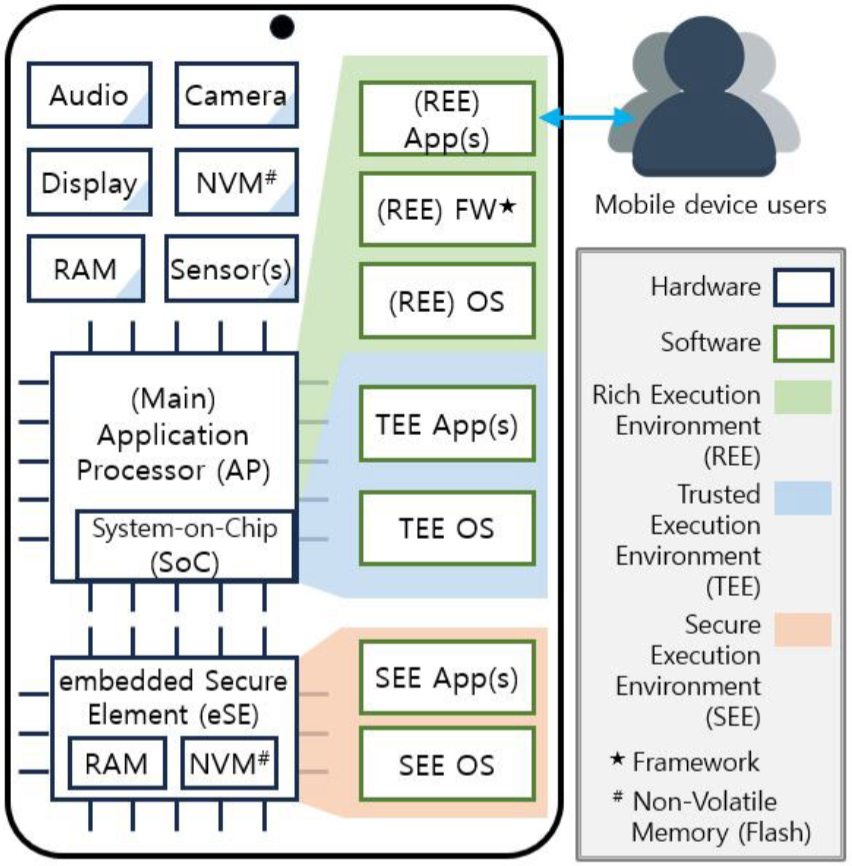
\includegraphics[width=0.3\textwidth]{figures/SecureElement.png}
    \caption{Secure element architecture.}
    \label{fig:SecureElement}
\end{figure}

\begin{table}[ht]
  \centering
  \caption{Total processing time comparison of drop-in replacement versus the proposed post-quantum cryptography migration scheme (values in milliseconds).}
  \label{tab:pqc_migration_total_time}
  \small
  \begin{tabular}{ll r}
    \toprule
    \textbf{Category} & \textbf{Scheme} & \textbf{Total} \\
    \midrule
    ML-DSA-44 & Drop-in replacement & 1,351 \\
              & Proposed scheme     &   933 \\
    \midrule
    ML-DSA-65 & Drop-in replacement & 1,826 \\
              & Proposed scheme     & 1,229 \\
    \midrule
    ML-DSA-87 & Drop-in replacement & 2,119 \\
              & Proposed scheme     & 1,445 \\
    \bottomrule
  \end{tabular}
\end{table}

\paragraph{Post-quantum Ligero signatures}
The next direction involved a full research on the actual state of the art of post-quantum signature schemes implementation.
Still keeping in mind our design choice to be compliant with the actual standards, we focused on the possibility to implement
other algorithm then ECDSA for the device binding signature, and other algorithm then ECDSA for the issuer signature. 
For the device binding signature, as Lehmann et al. pointed out in their paper Vision~\cite{Lehmann2025Vision}, current 
Secure Elements merely supports ECDSA signatures over P-256 curves. Moreover we needed the signature algorithm to be easily provable
with zero knowledge technique in order to enable user to selectively disclose the identity attributes of the credentials.

With respect to Ligero, no zero knowledge friendly post-quantum signature scheme has been implemented up to now.
There where other proving systems like zkVM, for example RiscZero~\cite{RiscZero2026} that we tested in order to prove basic claims, but their
run on android where extremely inefficient and not suitable for our purposes. We had to find another approach to solve the problem.

\paragraph{zkDilithium library}
This is where we had a fundamental intuition, which is actually one of the main contributions of this thesis to the current
state of the art. 
\begin{claim}
Post-quantum security for honest user does not require the device binding signature algorithm to be post-quantum secure.
\end{claim}
We can show this by modifying the actual Ligero circuit approach to the credential presentation problem.
Since Ligero is a zero knowledge proof system, in presentation moment the adversary is going to learn only that we know a valid
device signature which involves the device public key contained in the credential. Revealing device public key to the relying party
would lead to a privacy violation, since the relying party could link different presentations of the same credential.
The device public key is also involved in another operation: credential issuance. 
In this case, a semi-honest issuer could store user credential and user's device public key, and later on could break the device key
offline and clone his credentials on every smartphone, invalidating the device binding property.
To solve this problem, we came out with the following solution: the user will not send the issuer his device public key, 
but will instead send the sha256 of the device public key, and will prove in zero knowledge that he knows a valid preimage of the 
sha256. This way, the issuer will not be able to break the device key offline, since he does not know the device public key,
and the relying party will not be able to link different presentations of the same credential, since he does not know the device public key.

This direction allowed us to pass to the next step, which is to find a post-quantum signature scheme that is zk-friendly and can be used for the issuer signature.
The most promising candidate we found is zk-dilithium~\cite{policharla2023postquantum}, an open source library that implements
a zero knowledge friendly version of dilithium, a NIST standardized post-quantum signature scheme.
The paper's primary contribution is modifying the standard Dilithium (ML-DSA) algorithm to be efficient within a Zero-Knowledge 
proof system (specifically zkSTARKs). The main optimizations they introduce are:
\begin{itemize}
      \item \textbf{Hash Function Replacement}: Standard Dilithium uses SHA-3/SHAKE, which is very expensive to prove in ZK. 
      The paper replaces it with Poseidon, an algebraic hash function designed for STARK efficiency;
      \item \textbf{Public Key Distribution}: They do not use public key compression. By distributing the full vector t in 
      the public key, they eliminate the need for the complex "hint" h in the signature verification process;
      \item \textbf{"Sample In Ball" Optimization}: The deterministic algorithm used to generate challenges is modified to 
      avoid rejection sampling within the ZK circuit, significantly lowering the number of constraints needed.
\end{itemize}
Given this optimizations, the experimental results that the authors report in their paper are the provided in the table~\ref{tab:runtimes_memory} below.


\begin{table}[ht]
  \centering
  \caption{Run times and peak memory usage.}
  \label{tab:runtimes_memory}
  \small
  \begin{tabularx}{\textwidth}{@{}l X X X@{}}
    \toprule
    \textbf{Scheme} & \textbf{Prover (ms)} & \textbf{Verifier (ms)} & \textbf{Prover RAM (MB)} \\
    \midrule
    Better size & 4822 & 19.8 & 235 \\
    Balanced    & 660  & 22.0 & 40 \\
    Better time & 304  & 31.4 & 19 \\
    \bottomrule
  \end{tabularx}
\end{table}

The performance are completely compatible for our application, and the fact that the library is open source allows us to modify it 
and adapt it to our needs, which is a very good thing considering the fact that we need to connect it with Ligero and we need to
modify the public key field in the credential document standard.

Now the situation is the following: we have Ligero zero knowledge proof system which is optimized for proving sha256 preimage
and ECDSA, and we will use to prove device binding, disclose attributes ecc, and we have the zk-dilithium STARK prover
which we will use to prove issuer's signature over device credentials. The next question is how to connect the two proof systems, 
since we need to prove that the Ligero credentials that we disclose are the same proven to be signed by the issuer in the STARK proof,
and this is what we are going to show in the next two paragraphs.

\paragraph{SHA256 vs Poseidon}
This paragraph is going to show the problem we have to face in order to connect Ligero and zk-dilithium proof systems via a 
common commitment scheme.Immediately, we notice that this commitment should be both hiding and binding.

The first and simpler solution that came to our mind was to use a common, public sha256 commitment of the message signed by the issuer,
which corresponds to the hash of the credential. In this way, we just needed a public commitment, the same in the common public input
for both Ligero and STARK proof system, and we could prove in Ligero that the commitment is associated to the sha256 of the credential,
and in STARK that the commitment is associated to the issuer signature over the credential. Moreover, we had already the implementation
of the sha256 preimage prover in Ligero, and, as Frigo and Shelat shows in their paper~\cite{cryptoeprint:2024/2010}, the sha256 preimage
proof performance, that are reported in the table~\ref{tab:sha256_frigo_shelat} below, are completely compatible with our application.
\begin{table}[ht]
\centering
\caption{Timing benchmark of an n-block pre-image to the SHA-256 function performed on x86\_64 Emerald Rapids.}
\label{tab:sha256_frigo_shelat}
\small
\begin{tabularx}{\textwidth}{@{}l X X X X@{}}
\toprule
\textbf{Blocks (n)} & \textbf{Verify Transcript (ms)} & \textbf{Total ZK Prover (ms)} \\
\midrule
1 block  & 6.07  & 10.7 \\
2 blocks & 12.1  & 19.8 \\
4 blocks & 24.3  & 35.2 \\
8 blocks & 49.8  & 67.9 \\
\bottomrule
\end{tabularx}
\end{table}
The problem there became the following: how to implement sha256 inside the STARK prover system ? The answer was not trivial at all.
We searched for an efficient implementation of sha256 inside a STARK prover system, and we found the winterfell sha256 implementation
on github~\cite{iStrannikWinterfellSha256} which had good performance, but we found out a field incompatibility problem between the
winterfell sha256 implementation which was running on $GF(2^{128})$, and the zk-dilithium STARK implementation, which is a fork of 
the standard STARK winterfell implementation by Facebook~cite{FacebookWinterfell} running on $q = 2^{23} - 2^{20} + 1$ field.
The other way around was to implement the Poseidon hash function, which is implemented by default in the STARK proof system 
and runs in a few milliseconds, being poseidon a zk-friendly hash function. We searched online for a Ligero implementation of
the Poseidon23 hash function, which was the STARK version, but we were didn't find any implementation. Since the field in which
Poseidon23 function was implemented in the STARK proof system was different from the field in which Ligero was implemented, 
we decided to try to look for a simpler way to connect the two proof systems.

Notice that, whenever there will be an online implementation of Poseidon23 for Ligero, or sha256 for STARK in 
$q = 2^{23} - 2^{20} + 1$ field, we will be able to easily modify our solution to use the same hash function for both proof 
systems, which could lead to a possible speed up.

\paragraph{MAC code witness passing technique}
In this final paragraph we show how to connect the two proof systems without using a common hash function, 
but using an information theoretic MAC like Frigo and Shelat paper in section 3.4 of their paper~\cite{cryptoeprint:2024/2010}, 
which allows us to pass the sha256 of the credential from the Ligero circuit to the zk-dilithium STARK circuit in a secure way.
The idea is the following: the prover generates a random key $k_p$ and sends it to the verifier,
who generates a public key $k_v$ and send it back to the prover. The orchestrator computes the MAC as $MAC m = a*x + b$ over the
sha256 of the credential $x$, where $a$ and $b$ are obtained as $(a,b) = k$ with respect to the key $k = k_p \oplus k_v$. 
The prover shows in Ligero that he knows a valid preimage of the sha256 of the credential, and that the MAC is correct with respect 
to $k_p$ and $k_v$, and in STARK that he knows a valid signature of the issuer over a credential whose sha256 has a MAC equal to the 
one received from the orchestrator with respect to $k_p$ and $k_v$. T

his way, we can securely pass the sha256 of the credential from Ligero to zk-dilithium without using a common hash function, 
and without revealing any information about the credential itself.

Further proofs of security and formal implementation details are provided in the next sections.

\section{Proof Formalization}
\label{formalization}
In this section we are going to formalize how our design of the prover and the verifier works.

\subsection{Glossary of Symbols}
\label{sec:glossary}
% ═══════════════════════════════════════════════════════════════════════════

\paragraph*{Credential and session}

\begin{description}[leftmargin=3.5em, labelwidth=3em, style=sameline, itemsep=2pt]
  \item[$MSO$]   The user's credential (Mobile Security Object), a byte-string
                 laid out as an array of fields.
  \item[$tr$]    \emph{Session transcript}: a unique, fresh value jointly produced
                 by prover and verifier during the handshake. It binds the proof to
                 one specific session (anti-replay / freshness) and is the nonce the
                 device signs for device binding. Used in $k_v$ derivation and in
                 constraint \textbf{(L7)}.
  \item[$now$]   Current Unix timestamp, checked against the credential's validity
                 window \textbf{(L6)}.
  \item[$attr$]  The attribute value being disclosed.
  \item[$id$]    Index of $attr$ inside $MSO$.
\end{description}

\paragraph*{Credential hash and commitments}

\begin{description}[leftmargin=3.5em, labelwidth=3em, style=sameline, itemsep=2pt]
  \item[$e_1$]   $\SHA(MSO[0:183])$---the message the issuer actually signed.
                 Shared (privately) by both proofs.
  \item[$R_S$]   STARK-side Poseidon23 commitment to $(k_p,e_1)$. Locks the
                 prover's key share so $e_1$ cannot be swapped.
  \item[$R_L$]   Ligero-side SHA256 commitment to $(k_p,e_1)$. Same purpose,
                 on the other proof system.
\end{description}

\paragraph*{MAC (links the two proofs)}

\begin{description}[leftmargin=3.5em, labelwidth=3em, style=sameline, itemsep=2pt]
  \item[$k_p$]   Prover's secret key share, fresh per presentation (unlinkability).
  \item[$k_v$]   Verifier's key share, derived as
                 $\SHA(R_L \concat R_S \concat tr)$. Depends on \emph{both}
                 commitments, so it cannot be fixed before committing to $e_1$.
  \item[$a,b$]   The two 128-bit halves of $k_v \oplus k_p$ ($a = $ high,
                 $b = $ low); together they form the affine-MAC key.
  \item[$m$]     The \textbf{MAC tag} of $e_1$: $m = a \cdot e_1 + b \in \FF$.
                 It is an authentication tag---it neither hides nor encrypts
                 $e_1$. The \emph{same} $m$ appears in both proofs and is the
                 value the verifier cross-checks.
\end{description}

\paragraph*{Keys and signatures}

\begin{description}[leftmargin=3.5em, labelwidth=3em, style=sameline, itemsep=2pt]
  \item[$PK_{II}$]         Issuer public key (Dilithium, post-quantum).
  \item[$SK_{II}$]         Issuer secret key (Dilithium).
  \item[$sign$]            Issuer's Dilithium signature on $e_1$.
  \item[$pk_{dx},pk_{dy}$] Device public key (the two elliptic-curve coordinates
                           over P-256).
  \item[$(r_2,s_2)$]       Device's ECDSA-P256 signature over the session nonce,
                           proving device binding.
\end{description}

\paragraph*{Device-auth black boxes (Frigo--Shelat)}

\begin{description}[leftmargin=3.5em, labelwidth=3em, style=sameline, itemsep=2pt]
  \item[$H$]    The hash applied to $tr \concat hdr$ before the device ECDSA
                check (left unspecified; specified by Frigo--Shelat).
  \item[$hdr$]  The DeviceAuth header prepended to $tr$ (left unspecified).
\end{description}

\paragraph*{Outputs}

\begin{description}[leftmargin=3.5em, labelwidth=3em, style=sameline, itemsep=2pt]
  \item[$\pi_S,\pi_L$] The STARK and Ligero zero-knowledge proofs.
  \item[$Pres$]        The presentation $(X_S, X_L, \pi_S, \pi_L)$ handed to
                       the verifier.
\end{description}

% ═══════════════════════════════════════════════════════════════════════════
\subsection{Notation}
\label{sec:notation}
% ═══════════════════════════════════════════════════════════════════════════

\begin{center}
\renewcommand{\arraystretch}{1.35}
\begin{tabular}{@{}ll@{}}
\toprule
\textbf{Notation} & \textbf{Meaning} \\
\midrule
$x \concat y$                       & concatenation of bit-strings $x$ and $y$ \\
$[\,\mathit{cond}\,]$               & $1$ if $\mathit{cond}$ holds, $0$ otherwise \\
$z = \hipart{z} \concat \lopart{z}$ & for $z\in\FF$: $\hipart{z}, \lopart{z}$ are the most-/least-significant 128-bit halves \\
\bottomrule
\end{tabular}
\end{center}

% ═══════════════════════════════════════════════════════════════════════════
\subsection{Assumed Components}
\label{sec:components}
% ═══════════════════════════════════════════════════════════════════════════

\begin{align*}
\SHA            &: \text{byte-string} \to \{0,1\}^{256} \\
\Poseidon       &: \text{byte-string} \to \{0,1\}^{256} \\
H               &: \text{byte-string} \to \{0,1\}^{256}
  && \text{(Frigo--Shelat device check, unspecified)} \\
hdr             &: \text{byte-string}
  && \text{(DeviceAuth header, unspecified)} \\
\prand(n)       &: \mathbb{N} \to \{0,1\}^{8n}
  && \text{(\texttt{rand.randombytes(n)})} \\
\nowts()        &: () \to \mathbb{N}
  && \text{(\texttt{time.getTimestamp(0)}, current Unix time)} \\
\attrat(MSO,id) &: \text{byte-string} \times \mathbb{N} \to \text{byte-string}
  && \text{the $id$-th attribute element of $MSO$}
\end{align*}

\paragraph{Dilithium (post-quantum signature scheme).}
The issuer key pair is produced by $\DilKG$; the issuer signs the credential
hash with $\DilSign$; the relation \textbf{(S3)} checks the signature with
$\DilVerify$.
\begin{align*}
\DilKG()                         &\to (SK_{II},\, PK_{II}) \\
\DilSign(SK_{II},\, msg)         &\to sign \\
\DilVerify(sign,\, msg,\, PK_{II}) &\to \{0,1\}
\end{align*}

\paragraph{ECDSA over P-256 (device binding).}
The device key pair is produced by $ECKG$; the device signs the session
nonce $H(tr \concat hdr)$ with $ECSign$; the relation \textbf{(L7)} checks the
signature with $ECVerify$.
\begin{align*}
ECKG()                                                       &\to (sk_d,\, (pk_{dx}, pk_{dy})) \\
ECSign(sk_d,\, msg)                                          &\to (r_2,\, s_2) \\
ECVerify\!\bigl((r_2, s_2),\, msg,\, (pk_{dx}, pk_{dy})\bigr) &\to \{0,1\}
\end{align*}

% ═══════════════════════════════════════════════════════════════════════════
\subsection{Proof Systems}
\label{sec:proof-systems}
% ═══════════════════════════════════════════════════════════════════════════

\[
  \mathrm{Prove}(x, w) \to \pi
  \quad\textbf{require } (x,w)\in\mathcal{R};\quad
  \textbf{ensure } \mathrm{Verify}(x,\pi)=1,
\]
\[
  \mathrm{Verify}(x, \pi) \to b
  \quad\textbf{ensure } b=1 \;\Rightarrow\; \exists\, w'.\; (x,w')\in\mathcal{R}.
\]

% ───────────────────────────────────────────────────────────────────────────
\paragraph{Module \textsf{STARK}}
\label{sec:stark}
% ───────────────────────────────────────────────────────────────────────────

The STARK module proves issuer-credential validity and links the two proof
systems via the affine MAC. We name its instance $X_S$ and witness $W_S$.

\begin{mdframed}[style=relationbox]
{\small
\[
\RelSTARK \;=\; \left\{\;
\begin{array}{@{}l@{}}
x := (PK_{II},\, m,\, k_v,\, R_S) \\[5pt]
w := (sign,\, e_1,\, k_p,\, a,\, b)
\end{array}
\;\middle|\;
\begin{array}{@{}l@{\qquad}r@{}}
R_S = \Poseidon(k_p \oplus e_1) \;\wedge & \text{(S1)} \\[4pt]
a = \hipart{(k_v \oplus k_p)} \;\wedge & \text{(S2a)} \\[4pt]
b = \lopart{(k_v \oplus k_p)} \;\wedge & \text{(S2b)} \\[4pt]
m = a \cdot e_1 + b \;\wedge & \text{(S2c)} \\[4pt]
\DilVerify(sign,\, e_1,\, PK_{II}) = 1 & \text{(S3)}
\end{array}
\;\right\}
\]
}
\end{mdframed}

\begin{itemize}[leftmargin=2em, itemsep=2pt]
  \item \textbf{(S1)} $R_S$ is the STARK commitment opening of $(k_p, e_1)$.
  \item \textbf{(S2a),(S2b)} The MAC key halves $a,b$ are asserted to equal
        the high/low halves of $k_v \oplus k_p$; an incorrect $a$ or $b$
        makes the proof fail.
  \item \textbf{(S2c)} $m$ is the affine MAC of $e_1$ under that key.
  \item \textbf{(S3)} $sign$ is a valid Dilithium issuer signature on $e_1$.
\end{itemize}

% ───────────────────────────────────────────────────────────────────────────
\paragraph{Module \textsf{Ligero}}
\label{sec:ligero}
% ───────────────────────────────────────────────────────────────────────────

The Ligero module proves attribute disclosure, credential-to-device binding,
validity window, and device possession. We name its instance $X_L$ and
witness $W_L$.

\begin{mdframed}[style=relationbox]
\[
\resizebox{\linewidth}{!}{$\displaystyle
\RelLigero \;=\; \left\{\;
\begin{array}{@{}l@{}}
x := (attr,\, id,\, tr,\, now, \\
\phantom{x := (}\, m,\, k_v,\, R_L) \\[5pt]
w := (r_2,\, s_2,\, MSO,\, pk_{dx}, \\
\phantom{w := (}\, pk_{dy},\, k_p,\, e_1,\, a,\, b)
\end{array}
\;\middle|\;
\begin{array}{@{}l@{\quad}r@{}}
e_1 = \SHA(MSO[0:183]) \;\wedge & \text{(L1)} \\[4pt]
R_L = \SHA(k_p \oplus e_1) \;\wedge & \text{(L2)} \\[4pt]
a = \hipart{(k_v \oplus k_p)} \;\wedge & \text{(L3a)} \\[4pt]
b = \lopart{(k_v \oplus k_p)} \;\wedge & \text{(L3b)} \\[4pt]
m = a \cdot e_1 + b \;\wedge & \text{(L3c)} \\[4pt]
attr = \attrat(MSO, id) \;\wedge & \text{(L4)} \\[4pt]
MSO[128:160] = \SHA(pk_{dx} \concat pk_{dy}) \;\wedge & \text{(L5)} \\[4pt]
\intcast(MSO[48:56]) < now < \intcast(MSO[56:64]) \;\wedge & \text{(L6)} \\[4pt]
ECVerify\!\bigl((r_2,s_2),\, H(tr \concat hdr),\, (pk_{dx},pk_{dy})\bigr) = 1 & \text{(L7)}
\end{array}
\;\right\}
$}
\]
\end{mdframed}

\begin{itemize}[leftmargin=2em, itemsep=2pt]
  \item \textbf{(L1)} $e_1$ is the SHA256 hash of the credential $MSO$.
  \item \textbf{(L2)} $R_L$ is the Ligero commitment opening of $(k_p, e_1)$.
  \item \textbf{(L3a),(L3b),(L3c)} Same structure as \textbf{(S2a)--(S2c)}:
        $a, b$ are the high/low halves of $k_v \oplus k_p$, and
        $m = a \cdot e_1 + b$.
  \item \textbf{(L4)} $attr$ is the disclosed attribute at position $id$ in $MSO$.
  \item \textbf{(L5)} The device public key $(pk_{dx}, pk_{dy})$ hashes to the
        value stored in $MSO$.
  \item \textbf{(L6)} The current time $now$ lies within the credential's
        validity window.
  \item \textbf{(L7)} $(r_2, s_2)$ is a valid device ECDSA-P256 signature
        over the session nonce (device possession / binding).
\end{itemize}

% ═══════════════════════════════════════════════════════════════════════════
\subsection{Algorithm 1 --- Orchestrator}
\label{sec:orchestrator}
% ═══════════════════════════════════════════════════════════════════════════

\paragraph{The Orchestrator as a prover.} 

\begin{mdframed}[style=relationbox]
{\small
\[
\RelOrch \;=\; \left\{\;
\begin{array}{@{}l@{}}
x := (PK_{II},\, attr,\, id,\, tr,\, now, \\
\phantom{x := (}\, m,\, k_v,\, R_S,\, R_L) \\[5pt]
w := (sign,\, r_2,\, s_2,\, MSO,\, pk_{dx}, \\
\phantom{w := (}\, pk_{dy},\, e_1,\, k_p,\, a,\, b)
\end{array}
\;\middle|\;
\begin{array}{@{}l@{\quad}r@{}}
k_v = \SHA(R_L \concat R_S \concat tr) \;\wedge & \text{(O1)} \\[5pt]
\bigl(X_S,\, W_S\bigr) \in \RelSTARK \;\wedge & \text{(O2)} \\[5pt]
\bigl(X_L,\, W_L\bigr) \in \RelLigero & \text{(O3)}
\end{array}
\;\right\}
\]
}
\end{mdframed}

\noindent where the sub-instances and sub-witnesses are the projections
\[
\begin{aligned}
X_S &= (PK_{II},\, m,\, k_v,\, R_S), &\qquad
W_S &= (sign,\, e_1,\, k_p,\, a,\, b), \\
X_L &= (attr,\, id,\, tr,\, now,\, m,\, k_v,\, R_L), &\qquad
W_L &= (r_2,\, s_2,\, MSO,\, pk_{dx},\, pk_{dy},\, k_p,\, e_1,\, a,\, b).
\end{aligned}
\]

\begin{remark}
The only constraint not already enforced by $\RelSTARK$ or $\RelLigero$ is
\textbf{(O1)}, the derivation of the verifier key $k_v$. Constraint
\textbf{(O1)} binds \emph{both} commitments $R_S, R_L$ and the session
transcript $tr$ together, so $k_v$ cannot be fixed before committing to $e_1$.
Every other property---the issuer signature \textbf{(S3)}, the device
signature \textbf{(L7)}, the affine MAC \textbf{(S2c)/(L3c)}, the validity
window \textbf{(L6)}, and so on---is inherited from the two sub-relations.
Because $\RelOrch$ uses a single shared witness, the values $e_1, k_p, a, b, m$
and $k_v$ are automatically forced to agree across the STARK and Ligero
instances.
\end{remark}

\begin{algorithm}[H]
\caption{Orchestrator (prover for $\RelOrch$)}
\label{alg:orchestrator}
\begin{algorithmic}[1]
\Require $MSO$,\; $tr$,\; device signature $(r_2, s_2)$,\; issuer signature $sign$,\;
         device public key $(pk_{dx}, pk_{dy})$,\;
         attribute $attr$ with index $id$,\; issuer public key $PK_{II}$
\Ensure  $Pres = (X_S, X_L, \pi_S, \pi_L)$
\State $e_1 \gets \SHA(MSO[0:183])$
\State $k_p \gets \prand(32)$
\State
\State $R_S \gets \Poseidon(k_p \oplus e_1)$
\State $R_L \gets \SHA(k_p \oplus e_1)$
\State $k_v \gets \SHA(R_L \concat R_S \concat tr)$
  \Comment{establishes \textbf{(O1)}}
\State
\State $a \gets \hipart{(k_v \oplus k_p)}$
\State $b \gets \lopart{(k_v \oplus k_p)}$
\State $m \gets a \cdot e_1 + b$
\State
\State $now \gets \nowts()$
\State
\State $X_S \gets (PK_{II},\; m,\; k_v,\; R_S)$
\State $W_S \gets (sign,\; e_1,\; k_p,\; a,\; b)$
\State $X_L \gets (attr,\; id,\; tr,\; now,\; m,\; k_v,\; R_L)$
\State $W_L \gets (r_2,\; s_2,\; MSO,\; pk_{dx},\; pk_{dy},\; k_p,\; e_1,\; a,\; b)$
\State
\State \(\triangleright\)~\textit{Pre-condition (cf.\ $\RelOrch$): $(X_S,W_S)\in\RelSTARK$ and
       $(X_L,W_L)\in\RelLigero$}
\State $(\pi_S, \pi_L) \gets
  \mathrm{parallel}\!\bigl(
    ()\mapsto\STARKProve(X_S,W_S),\;
    ()\mapsto\LigeroProve(X_L,W_L)
  \bigr)$
\State \Return $(X_S, X_L, \pi_S, \pi_L)$
\end{algorithmic}
\end{algorithm}

% ═══════════════════════════════════════════════════════════════════════════
\subsection{Algorithm 2 --- Verifier}
\label{sec:verifier}
% ═══════════════════════════════════════════════════════════════════════════

\paragraph{What the verifier checks.}
On receiving a presentation $Pres = (X_S, X_L, \pi_S, \pi_L)$ and session
transcript $tr$, the verifier accepts iff a witness for the Orchestrator
relation $\RelOrch$ exists for the implied statement. Concretely it verifies
the four properties below; the first that fails causes rejection.

\begin{enumerate}[leftmargin=2em, label=\textbf{V\arabic*.}, itemsep=3pt]
  \item \textbf{Consistency.} Both proofs share the same MAC tag $m$, the same
        verifier key $k_v$, and the same session transcript $tr$
        ($m_S = m_L$,\; $k_{v,S} = k_{v,L}$,\; $tr_L = tr$). This forces the two
        instances to be the projections $X_S, X_L$ of a single Orchestrator
        instance, preventing an adversary from mixing components of different
        sessions or credentials.
  \item \textbf{Binding of $k_v$ (constraint \textbf{(O1)}).} The verifier key is
        the hash of \emph{both} commitments together with the transcript,
        $k_v = \SHA(R_L \concat R_S \concat tr)$. This is exactly the additional
        constraint of $\RelOrch$ and is the one property that neither
        sub-proof checks internally.
  \item \textbf{STARK validity (constraint \textbf{(O2)}).} The proof $\pi_S$ is a
        valid proof of knowledge for $X_S$: there exists $W_S$ with
        $(X_S, W_S)\in\RelSTARK$. This certifies the issuer Dilithium signature
        on $e_1$ and the correct MAC computation.
  \item \textbf{Ligero validity (constraint \textbf{(O3)}).} The proof $\pi_L$ is a
        valid proof of knowledge for $X_L$: there exists $W_L$ with
        $(X_L, W_L)\in\RelLigero$. This certifies attribute disclosure, device
        binding, and credential freshness.
\end{enumerate}

Conditions \textbf{V1}--\textbf{V4} together establish that there exists a
witness $W_{\mathsf{Orch}}$ with $\bigl((X_S\cup X_L),\, W_{\mathsf{Orch}}\bigr)
\in \RelOrch$: \textbf{V1} identifies the shared public values, \textbf{V2}
discharges the additional constraint \textbf{(O1)}, and \textbf{V3}--\textbf{V4}
discharge \textbf{(O2)}--\textbf{(O3)}.

\begin{algorithm}[H]
\caption{Verifier}
\label{alg:verifier}
\begin{algorithmic}[1]
\Require $Pres$,\; session transcript $tr$
\Ensure $\accept$ or $\reject$
\State \Parse $Pres = (X_S, X_L, \pi_S, \pi_L)$
\State \Parse $X_S = (PK_{II},\; m_S,\; k_{v,S},\; R_S)$
\State \Parse $X_L = (attr,\; id,\; tr_L,\; now,\; m_L,\; k_{v,L},\; R_L)$
\State
\State \(\triangleright\)~\textit{V1: consistency --- shared MAC, verifier key, and session}
\If{$m_S \neq m_L$} \Rejects \EndIf
\If{$k_{v,S} \neq k_{v,L}$} \Rejects \EndIf
\If{$tr_L \neq tr$} \Rejects \EndIf
\State
\State \(\triangleright\)~\textit{V2: binding --- constraint (O1) of $\RelOrch$}
\If{$k_{v,S} \neq \SHA(R_L \concat R_S \concat tr)$} \Rejects \EndIf
\State
\State \(\triangleright\)~\textit{V3: STARK proof validity --- constraint (O2)}
\If{$\STARKVerify(X_S, \pi_S) \neq 1$} \Rejects \EndIf
\State
\State \(\triangleright\)~\textit{V4: Ligero proof validity --- constraint (O3)}
\If{$\LigeroVerify(X_L, \pi_L) \neq 1$} \Rejects \EndIf
\State
\Accepts
\end{algorithmic}
\end{algorithm}


\section{Security Analysis}
\label{analysis}
In this section we are going to perform analysis with respect to the security of our solution, we are going to analyze
the compliance of our solution with the eIDAS 2.0 regulation and with the LoA High requirements, and we are going to analyze 
the threat model of our solution, showing how and why it satisfies our design choice explained in section~\ref{designchoice}.

\subsection{MAC Witness Sharing}
\label{securityanalysis}
STARK zk proof over the issuer signature needs dilithium verification algorithm.
The algorithm takes in input the signature $sig$, the message being signed $e_1$ and 
the public key of the issuer $PK_{II}$.
The message signed by the issuer $e_1$is the sha256 of the credential document. Knowledge
of sha256 preimage is hard to prove in STARK winterfell circuit, so we propose the
following solution: the Ligero circuit, which has an optimized sha prover, will
prove $e_1 = sha256(cred)$, then $e_1$ is encoded in a binding and hiding commitment
realized with information theoretic MAC.

Mathematical proof of MAC security:$$m = MAC_k(e_1) = MAC_{k_p,k_v}(e_1) = MAC_{a,b}(e_1)$$
We obtain the key as:$$(a,b) = k_p \oplus k_v$$ where $k_p$ is a secret random 32 bytes key
chosen by the prover and $k_v$ is a public verifiable key chosen by the verifier.
What security concerns do we have?
\begin{enumerate}
    \item The prover can try to forge a valid MAC for a different $e_1'$, but $e_1'$ would
    still need to be a valid sha256 of signed credential since the signature is verified by the circuit;
    \item The prover could generate $k_p$ after seeing $k_v$, leading to arbitrary proves;
    \item Different presentations could be linkable to the same MAC.
\end{enumerate}
2 is avoidable if we require the prover to generate $k_p$ before seeing $k_v$, committing to 
and building $k_v$ with fiat shamir transform on $k_p$ commitment, and 3 is avoidable if we require the 
prover to generate a different $k_p$ for each presentation.

For 1, we have the following security proof in which we show that is not possible to forge 
a valid MAC for a different $e_1'$ without breaking the security of the MAC scheme:
$$m = MAC_k(e_1) = a*e_1 + b = a*e_1' + b \Rightarrow a*(e_1 - e_1') = 0$$
which is true either if a = 0 or if $e_1 = e_1'$. It has been proven that the probability
that $a = 0$ is negligible.
if $e_1 = e_1'$ then the prover is proving the same credential, so no forgery is happening.
We also now that is not possible to have $m_1 = a'*e_1 + b' = m_2 = a''*e_1' + b''$ since
the prover is not able to choose $a$ and $b$ due to the verifier participation in the key
generation with $k_v$.
\subsection{Compliance with eIDAS 2.0 and LoA High}
\label{ComplianceEIDAS}
In this section we are going to analyze our solution, taking into account the requirements
of the European Commission for the EUDI wallet application, considering both the eIDAS 2.0
regulation and the LoA High (Level of Assurance High).

\paragraph{Dynamic Authentication and Replay Protection}$\newline$
CIR 2015/1502 requires that for LoA High, authentication must be dynamic, creating a proof 
that changes with each session. The plan fulfills this by including a session transcript (tr) 
in the Device Binding proof. The device's Secure Element signs this transcript, and the ZK 
circuit verifies this signature (p256.verify), ensuring the proof cannot be replayed by an 
attacker who has intercepted a previous proof.

\paragraph{Hardware Binding}$\newline$
The plan enforces Device Binding by extracting the public key ($pk_d$) from the signed MSO 
and requiring a proof of possession of the corresponding private key. This ensures the 
credential is bound to a tamper-resistant WSCD (Wallet Secure Cryptographic Device).
    
\paragraph{Algorithmic Soundness}$\newline$
The extraction error of the combined STARK/Ligero system is negligible
($O(\eta + d \cdot \log(w) / \mid F \mid)$), providing a robust mathematical barrier against forgery.

\paragraph{Compliance with EUDI ARF Requirements}$\newline$
The implementation satisfies several High-Level Requirements (HLRs) from the EUDI Architecture and Reference Framework:
\begin{itemize}
\item \textbf{User Sole Control}: The ZKP generation happens entirely on the user's device (orchestrated by the Wallet Unit),
 ensuring the user has sole control over attribute disclosure;
\item \textbf{Validity Verification}: The circuit enforces validity checks (tstart<tnow<tend) without revealing the actual 
issuance or expiration dates, as required for privacy-preserving interactions;
\end{itemize}

\subsection{Threat Model}
\label{threatmodel}
In this section we clarify the threat model we are considering for our solution, and explaining
clearly where this thesis is going to be placed inside the context of the EUDI wallet application.

Current implementations completely lacks of post-quantum security, since current infrastructures relies on
RSA and ECDSA signatures, and since hardware constraints of the LoA High requirements of the eIDAS 2.0 regulation
forces the use of P256 curve. Since now, for this reasons, no one has already made any steps in the direction
of getting a post-quantum solution for the EUDI wallet application.

With the solution proposed in this thesis, we are not achieving a full post-quantum secure wallet:
instead, what we are achieving is post-quantum security for the current state of the art and technology advance
in the quantum computing research.
In this moment, no quantum computer is able to break RSA nor ECDSA signatures, but what an adversary could do
is to record authentication sessions as a relying party or just a passive network monitoring adversary, and 
later on get the capability to break the signatures and forge device binding and issuer signature, or worst.
A malicious issuer could collect users device public key and credentials,
and later on break that set of keys and, being able to forge also device binding signature, impersonate other users.

With our solution we are protecting millions of users from this kind of risks. In fact, this solution is completely
secure assuming honest users, as shown before.
Why our solution is not actual secure against dishonest users?

\paragraph{Forgery attack}
A malicious prover, which owns a valid credential and owns a quantum computer, could reverse engineer the application
and extract the public key of the device. This is possible because, when the proof is generated, the device public key
is needed in order to generate the zero-knowledge proof for the validity of the device binding signature. This operation,
given the actual hardware restriction, cannot be made inside the Secure Element, therefore the device public key is
exposed to the wallet unit which runs the prover algorithm, and with proper technique could be extracted and reversed
with the Shor's algorithm~\cite{Shor1997Polynomial} in order to obtain the device private key.

\paragraph{Mitigation}
This attack allows a malicious prover to extract the device public key from his own device.
In order for the attacker to be able to use the stolen device keys, he will still need the credentials.
In the particular (and easier) case in which the attacker is the owner of the device and the credentials,
he will be able to pass his credentials across different devices and therefore he could allow other
users to use his credentials. This violates the LoA High required by the eIDAS 2.0 regulation, but does
not allow the attacker to impersonate other users, since he will not be able to forge device binding signature
for other users. Instead the attacker is only able to share his identity, which in first place harm his own
privacy. There is also a sever economic disincentive for the attacker to forge his own device keys, sincea 
this implies a quantum computer attack, expensive and time consuming, in order to forge a single keypair,
which by the way is his own keypair.

In conclusion, the solution proposed in this thesis is secure assuming honest users,
but is a perfect bridge between a completely quantum-agnostic implementation of the wallet and a future
post-quantum sound implementation of the wallet, which will be able to protect users against malicious quantum adversaries.
Post-quantum sound solutions are likely to be out soon, since the entire online community, due to incurrent quantum
threat, is moving towards post-quantum secure software. In particular, Google declared that the next version
of their operating system, Android 17, will implement post-quantum secure NIST standardized algorithm 
ML-DSA~\cite{Google2026SecurityQuantumAndroid}.


\section{Summary}
To summarize our solution: we designed a zero-knowledge proof system
composed by an orchestrator (prover) which runs two provers in parallel:
\begin{itemize}
  \item \textbf{Ligero}: Longfellow Ligero implementation, without proving issuer signature,
  and an additional MAC witness sharing circuit and commitment check, sha256 proof over device public key commitment
  on credentials;
  \item \textbf{STARK}: zk-dilithium circuit, without message sharing, with an additional MAC witness sharing circuit
  and commitment check;
\end{itemize}
We also designed a verifier which will ensure the MAC is the same and fill the two circuits input.

Moreover, we modified the standard MDOC document, replacing the old
device public key (2 coordinates, ECDSA keys, 256bits each) with their hash value obtained 
evaluating the sha256 function over each coordinate,,
without requiring any MDOC modification and keeping our protocol 100\% compatible
with ISO 18013-5 standard.

Therefore, we managed to design and implement a post-quantum
anonymous credential system for honest users. 

\chapter{Experimental Results}
\label{results}
In this section we report the empirical evaluation of our solution. Rather than
presenting only the final system, we benchmark the whole \emph{path} that led to
it: the unmodified building blocks (Longfellow and zkDilithium), the two hash
primitives we tried to use as a common commitment (SHA-256 and Poseidon23), the
incremental cost of each customization (removing message sharing from the STARK,
adding the SHA-256 opening to Ligero, and the MAC witness-sharing bridge), and
finally the cost of composing the two proof systems sequentially versus in
parallel. This experimental results are shown in order to justify the implementations choices
made in section~\ref{implementation}.

\section{Testing Setup}
\label{results:setup}
All experiments were run on three platforms: one desktop and the two
smartphones mandated by the device-binding use case.
\begin{itemize}[noitemsep]
  \item \textbf{Desktop} --- AMD Ryzen~5~1600 (6 cores / 12 threads, 3.2\,GHz),
        Linux, \texttt{x86\_64}.
  \item \textbf{Galaxy S24} --- Samsung SM-S928B, Qualcomm Snapdragon~8~Gen~3
        (\texttt{SM8650}), \texttt{arm64-v8a}.
  \item \textbf{Galaxy A53} --- Samsung SM-A536B, Samsung Exynos~1280
        (\texttt{s5e8825}), \texttt{arm64-v8a}, a mid-range device included to
        show behaviour on weaker hardware.
\end{itemize}
The smartphones represents an top-of-the-line Samsung device 2 years old 
and a mid-range Samsung device which is 5 years old, in order to show the 
performance of our solution on different hardware.

\paragraph{Methodology.} Every binary was compiled in release mode; the STARK
prover used its concurrent (multi-threaded) backend. Each cell of every table is
the \textbf{median of 5 runs}. For the Ligero/Longfellow prover, which compiles
and caches its arithmetic circuit on first use, we always discard the first
(cold-cache) run and report \emph{warm-cache} timings; the one-time circuit
generation is reported separately. Desktop timings were taken with the machine
otherwise idle, as we observed that a concurrent compilation could inflate a
STARK proving time by up to $5\times$. Unless stated otherwise, the credential
is the reference mDOC test vector disclosing a single attribute
(\texttt{age\_over\_18}), and the prover key share $k_p$ is fixed to simplify 
the analysis. Reported security levels are the conjectured ones: $115$~bit for
the zkDilithium STARK, ${\approx}96$~bit for the standalone SHA-256 STARK, and
the Longfellow default for the Ligero proofs.

\section{Build and Run Commands}
\label{results:repro}
For completeness, and so that every figure in this chapter can be reproduced from
the public repository, we list here the exact commands used to compile and run
each component on both target platforms --- the desktop (Linux, \texttt{x86\_64})
and the two Android phones (\texttt{arm64-v8a}). The Android cross-builds all use
the NDK r28 toolchain; below we write \texttt{\$ANDROID\_NDK\_ROOT} for its
install directory and \texttt{\$NDK} for its host \texttt{prebuilt} sub-path. The
mDOC test vector, the disclosed attribute (\texttt{age\_over\_18}) and the fixed
prover key share $k_p$ are the same across all runs, as stated in the methodology
above.

\paragraph{Longfellow mDOC proof (Ligero, C++).}
On the desktop the Ligero side is a CMake/Clang build; the \texttt{mdoc\_zk\_test}
target produces the warm-cache prove/verify timings of
\cref{tab:res-base-ligero}.
\begin{lstlisting}[caption={Longfellow mDOC proof (Ligero, C++): desktop build and run.},label={lst:ligero-desktop}]
# Desktop (Linux, x86_64)
cd longfellow-zk
CXX=clang++ cmake -D CMAKE_BUILD_TYPE=Release \
    -S lib -B clang-build-release --install-prefix ${PWD}/install
make -C clang-build-release mdoc_zk_test mdoc_signature_test -j8
./clang-build-release/circuits/mdoc/mdoc_zk_test \
    --gtest_filter='MdocZKTest.split_phase_roundtrip'
\end{lstlisting}
The Android cross-build first runs \texttt{android.sh} (which builds GoogleTest,
google-benchmark, zstd and OpenSSL for \texttt{arm64-v8a} into
\texttt{deps-android/}), then reconfigures out-of-tree because the committed
\texttt{CMakeCache.txt} carries a stale absolute source path; the
\texttt{-llog} linker flag is required because the minimal targets reference
\texttt{\_\_android\_log\_print}.
\begin{lstlisting}[caption={Longfellow mDOC proof (Ligero, C++): Android (arm64-v8a) cross-build and run.},label={lst:ligero-android}]
# Android (arm64-v8a)
export ANDROID_NDK_ROOT=$HOME/Android/Sdk/ndk/28.2.13676358
cd longfellow-zk
./android.sh
cmake -S lib -B /tmp/lf-android \
    -DCMAKE_TOOLCHAIN_FILE=$ANDROID_NDK_ROOT/build/cmake/android.toolchain.cmake \
    -DANDROID_ABI=arm64-v8a -DANDROID_PLATFORM=android-24 \
    -DCMAKE_BUILD_TYPE=Release \
    -DCMAKE_FIND_ROOT_PATH=$PWD/deps-android \
    -DCMAKE_EXE_LINKER_FLAGS=-llog
make -C /tmp/lf-android mdoc_zk_test -j8
adb push /tmp/lf-android/circuits/mdoc/mdoc_zk_test /data/local/tmp/
adb shell 'cd /data/local/tmp && ./mdoc_zk_test \
    --gtest_filter=MdocZKTest.split_phase_roundtrip'
\end{lstlisting}

\paragraph{zkDilithium signature proof (STARK, Rust).}
The STARK side is a Rust crate. The desktop build is a plain
\texttt{cargo build --release}; for Android we override the NDK linker and
archiver on the command line, since the crate's checked-in
\texttt{.cargo/config.toml} points at a different NDK location.
\begin{lstlisting}[caption={zkDilithium signature proof (STARK, Rust): desktop and Android.},label={lst:stark}]
# Desktop (Linux, x86_64)
cd zkdilithium
cargo build --release
RUST_LOG=info ./target/release/zk_dilithium

# Android (arm64-v8a)
export NDK=$HOME/Android/Sdk/ndk/28.2.13676358/toolchains/llvm/prebuilt/linux-x86_64
CARGO_TARGET_AARCH64_LINUX_ANDROID_LINKER=$NDK/bin/aarch64-linux-android29-clang \
CC_aarch64_linux_android=$NDK/bin/aarch64-linux-android29-clang \
AR_aarch64_linux_android=$NDK/bin/llvm-ar \
    cargo build --release --target aarch64-linux-android
adb push target/aarch64-linux-android/release/zk_dilithium /data/local/tmp/
adb shell 'cd /data/local/tmp && RUST_LOG=info ./zk_dilithium'
\end{lstlisting}

\paragraph{SHA-256-in-STARK proof-size sweep.}
The sensitivity study of \cref{tab:res-hash} is produced by the
\texttt{winterfell-sha256} prototype, whose \texttt{benchmark\_preimage} binary
sweeps the STARK parameters on the desktop, while the
\texttt{android\_prover}/\texttt{android\_verifier} pair reproduces the on-device
prove/verify timings of \cref{tab:res-hash}.
\begin{lstlisting}[caption={SHA-256-in-STARK parameter sweep and on-device prove/verify timings.},label={lst:sweep}]
# Desktop (Linux, x86_64)
cd winterfell-sha256
cargo run --release --features concurrent --bin benchmark_preimage

# Android (arm64-v8a): split prover / verifier
cargo build --release --features concurrent \
    --target aarch64-linux-android --bin android_prover --bin android_verifier
adb push target/aarch64-linux-android/release/android_prover  /data/local/tmp/
adb push target/aarch64-linux-android/release/android_verifier /data/local/tmp/
adb shell 'cd /data/local/tmp && ./android_prover && ./android_verifier'
\end{lstlisting}

\paragraph{Joint presentation (orchestrator).}
Finally, the full joint proof of \cref{tab:res-orchestrator} is driven by the
Rust orchestrator, which runs the STARK and Ligero provers in parallel. On the
desktop the Longfellow static library must be built first (see
Listing~\ref{lst:ligero-desktop}); on Android the binary additionally needs the
NDK's
\texttt{libc++\_shared.so} pushed alongside it.
\begin{lstlisting}[caption={Joint presentation (orchestrator, STARK${+}$Ligero in parallel): desktop and Android.},label={lst:orch}]
# Desktop (Linux, x86_64)
cargo build --release --manifest-path orchestrator/Cargo.toml
RUST_LOG=info ./orchestrator/target/release/pqac_orchestrator

# Android (arm64-v8a)
cd orchestrator
cargo build --release --target aarch64-linux-android
adb push target/aarch64-linux-android/release/pqac_orchestrator /data/local/tmp/
adb push $NDK/sysroot/usr/lib/aarch64-linux-android/libc++_shared.so \
    /data/local/tmp/
adb shell 'cd /data/local/tmp && LD_LIBRARY_PATH=/data/local/tmp \
    RUST_LOG=info ./pqac_orchestrator'
\end{lstlisting}
On a stock device the circuit cache directory may not be writable; in that case
each run pays a one-time cold-cache circuit regeneration (\(\sim\)30\,s on the
A53) before the warm timings reported here. All desktop measurements were taken
with the machine otherwise idle, as a concurrent compilation was observed to
inflate a STARK proving time by up to $5\times$.

\section{STARK and Ligero Default Run}
\label{results:baselines}
Before measuring the cost of any of our modifications we characterize the two
systems we build upon, exactly as they ship upstream: the Longfellow mDOC proof
(Ligero) and the zkDilithium signature proof (STARK). These two systems are the
references against which every customization in
\cref{results:customizations} is measured, so we report them in full detail and
on each of the three platforms separately rather than collapsing them into a
single average. As a sanity check, our desktop Longfellow numbers
($\sim$1.05\,s prove, $\sim$0.56\,s verify) sit in the same range as the figures
reported by Frigo and Shelat (\cref{tab:prover_verifier_perf}), and our
zkDilithium numbers are consistent with the original library
(\cref{tab:runtimes_memory}); this cross-check gives us confidence that our
measurement harness is sound before we start perturbing it.

\Cref{tab:res-base-ligero} reports the Longfellow mDOC baseline. Besides the raw
prove/verify/size triple we add two derived quantities that we will track
throughout the section: the \emph{verify/prove ratio}, which captures how
balanced the two phases are, and the \emph{prove time relative to the
Galaxy~S24}, which we adopt as the reference device because it is the
fastest prover on this workload.

\begin{table}[ht]
  \centering
  \caption{Longfellow mDOC (Ligero) baseline, per platform. Median of 5 runs,
  warm cache, single disclosed attribute. ``V/P'' is the verify-to-prove ratio;
  ``Prove rel.'' is the prove time normalised to the Galaxy~S24.}
  \label{tab:res-base-ligero}
  \small
  \begin{tabular}{@{}lrrrrr@{}}
    \toprule
    \textbf{Platform} & \textbf{Prove (ms)} & \textbf{Verify (ms)} & \textbf{Size (KB)} & \textbf{V/P} & \textbf{Prove rel.} \\
    \midrule
    Desktop    & 1047 & 559  & 351.6 & 0.53 & $1.08\times$ \\
    Galaxy S24 & 973  & 530  & 351.6 & 0.54 & $1.00\times$ \\
    Galaxy A53 & 1822 & 1099 & 351.6 & 0.60 & $1.87\times$ \\
    \bottomrule
  \end{tabular}
\end{table}

A first non-obvious observation is that the Galaxy~S24 is \emph{faster than our
desktop} on the Longfellow proof (973\,ms vs 1047\,ms): the Snapdragon~8~Gen~3
big cores outperform a 2017-era Ryzen on this MPC-in-the-head workload, which is
exactly the encouraging direction for a scheme meant to run on phones. 

The verify/prove ratio is remarkably stable across platforms (0.53--0.60), telling us
that verification is \emph{not} a fixed-cost overhead but scales with the same
hardware factors as proving. The proof size is, as expected for Ligero, completely
platform-independent at $351.6$\,KB.

\Cref{tab:res-base-stark} reports the zkDilithium STARK baseline. Here we
normalise the prove time to the \emph{Desktop}, which is the fastest STARK prover,
and we observe the opposite hardware story to Ligero.

\begin{table}[ht]
  \centering
  \caption{zkDilithium (STARK) baseline, per platform. Median of 5 runs,
  concurrent prover backend. ``Prove rel.'' is normalised to the Desktop.}
  \label{tab:res-base-stark}
  \small
  \begin{tabular}{@{}lrrrrr@{}}
    \toprule
    \textbf{Platform} & \textbf{Prove (ms)} & \textbf{Verify (ms)} & \textbf{Size (KB)} & \textbf{V/P} & \textbf{Prove rel.} \\
    \midrule
    Desktop    & 225 & 33.5 & 173.7 & 0.149 & $1.00\times$ \\
    Galaxy S24 & 369 & 39.7 & 173.7 & 0.108 & $1.64\times$ \\
    Galaxy A53 & 432 & 40.6 & 173.7 & 0.094 & $1.92\times$ \\
    \bottomrule
  \end{tabular}
\end{table}

Two points deserve emphasis. First, the STARK verify/prove ratio is an order of
magnitude smaller than Ligero's (0.09--0.15 versus 0.53--0.60): STARK
verification is genuinely cheap and almost flat across devices ($33$--$41$\,ms),
which is the classic STARK asymmetry of a relatively heavy prover paired with a
light verifier. Second, and in contrast to the Longfellow proof, here the desktop
\emph{wins}: the STARK prover is more sensitive to single-thread throughput and
to the small $\mathbb{F}_{2^{23}-2^{20}+1}$ field arithmetic, where the desktop's
wider out-of-order core still has an edge over the phone SoCs. The A53 is only
$1.92\times$ slower than the desktop on the STARK, against $1.87\times$ on Ligero,
so the mid-range gap is consistent across both proof systems and stays below
$2\times$ --- a useful invariant when we later reason about the joint proof on
weak hardware.

\section{SHA-256 vs Poseidon Running Times}
\label{results:hash}
As explained in \cref{implementation}, linking the two proofs requires committing
to the same credential hash $e_1$ on both sides, which initially meant proving
the \emph{same} hash function in both proof systems. \Cref{tab:res-hash}
quantifies why this turned out to be impractical. Proving a single SHA-256 block
inside the STARK costs $0.67$--$2.3$\,s depending on the device --- two orders of
magnitude more than the ${\approx}11$\,ms that the same SHA-256 block costs in
Ligero (\cref{tab:sha256_frigo_shelat}). Poseidon23, on the other hand, is cheap
\emph{everywhere}: as a STARK commitment it is essentially free (it adds at most
a few tens of milliseconds over the bare signature proof, see
\cref{tab:res-stark-steps}), and as a standalone Ligero preimage proof it costs
only $\sim$25--40\,ms.

\begin{table}[ht]
  \centering
  \caption{Cost of proving one hash invocation in each proof system. The SHA-256
  in-Ligero figure is the Frigo--Shelat reference (\cref{tab:sha256_frigo_shelat},
  x86); all others are measured in this work (median of 5).}
  \label{tab:res-hash}
  \small
  \begin{tabular}{@{}llrrr@{}}
    \toprule
    \textbf{Hash / proof system} & \textbf{Platform} & \textbf{Prove (ms)} & \textbf{Verify (ms)} & \textbf{Size (KB)} \\
    \midrule
    \multirow{3}{*}{SHA-256 in STARK (1 block)}
        & Desktop    & 666  & 118 & 73.2 \\
        & Galaxy S24 & 1207 & 294 & 73.2 \\
        & Galaxy A53 & 2287 & 522 & 73.2 \\
    \midrule
    SHA-256 in Ligero (1 block) & x86 (Frigo--Shelat) & \multicolumn{1}{r}{$\approx 11$} & \multicolumn{1}{r}{$\approx 6$} & --- \\
    \midrule
    \multirow{3}{*}{Poseidon23 in Ligero}
        & Desktop    & 25.5 & 12.7 & 77.7 \\
        & Galaxy S24 & 28.8 & 12.0 & 77.3 \\
        & Galaxy A53 & 38.5 & 16.0 & 77.3 \\
    \bottomrule
  \end{tabular}
\end{table}

The conclusion is the one anticipated in \cref{implementation}: each hash is
cheap in \emph{one} system and prohibitive or unavailable in the other (there is
no Poseidon23 gadget for Ligero's field, and no efficient SHA-256 AIR for the
zkDilithium field $\mathbb{F}_{2^{23}-2^{20}+1}$). This asymmetry is precisely
what motivated abandoning a shared hash commitment in favour of the
information-theoretic MAC bridge.

% \subsection{Running times forSHA-256 in STARK}
% \label{results:hash-sweep}
% The timings in \cref{tab:res-hash} already rule SHA-256-in-STARK out on grounds of
% \emph{proving time}, but it is instructive to ask whether the picture could be
% rescued by tuning the STARK's own parameters --- after all, a STARK proof system
% exposes a number of knobs (the Reed--Solomon blow-up factor, the proof-of-work
% grinding factor, the field-extension degree, the FRI folding factor) that trade
% prover work, verifier work, soundness and proof size against one another. To
% answer this we built a standalone SHA-256 AIR on the
% \texttt{winterfell-sha256} prototype and swept each parameter independently
% around the default configuration (blow-up $8$, grinding $16$ bits, no field
% extension, folding $8$, a single $240$-bit pre-image block), measuring the
% resulting proof size. \Cref{tab:res-stark-sweep} reports the full sweep.

% \begin{table}[ht]
%   \centering
%   \caption{SHA-256-in-STARK proof-size sensitivity (\texttt{winterfell-sha256}
%   prototype, single block). Each group varies one parameter while the others are
%   held at the default configuration (\emph{italicised} row, $61.97$\,KB). Proof
%   size only; timing is reported in \cref{tab:res-hash}.}
%   \label{tab:res-stark-sweep}
%   \small
%   \begin{tabular}{@{}llrr@{}}
%     \toprule
%     \textbf{Swept parameter} & \textbf{Value} & \textbf{Proof (B)} & \textbf{Proof (KB)} \\
%     \midrule
%     \multirow{4}{*}{Blow-up factor}
%         & 8 \emph{(default)} & 63\,460 & \emph{61.97} \\
%         & 16                 & 68\,995 & 67.38 \\
%         & 32                 & 75\,687 & 73.91 \\
%         & 64                 & 80\,072 & 78.20 \\
%     \midrule
%     \multirow{6}{*}{Grinding factor (bits)}
%         & 8                  & 64\,259 & 62.75 \\
%         & 16 \emph{(default)}& 63\,460 & \emph{61.97} \\
%         & 20                 & 63\,616 & 62.13 \\
%         & 24                 & 63\,710 & 62.22 \\
%         & 28                 & 64\,160 & 62.66 \\
%         & 32                 & 63\,231 & 61.75 \\
%     \midrule
%     \multirow{3}{*}{Field-extension degree}
%         & 1 \emph{(default)} & 63\,460 & \emph{61.97} \\
%         & 2                  & 72\,900 & 71.19 \\
%         & 3                  & 82\,147 & 80.22 \\
%     \midrule
%     \multirow{2}{*}{Folding factor}
%         & 8 \emph{(default)} & 63\,460 & \emph{61.97} \\
%         & 16                 & 61\,339 & 59.90 \\
%     \midrule
%     \multirow{9}{*}{Pre-image length (bits)}
%         & 110                & 58\,242 & 56.88 \\
%         & 240 \emph{(default)}& 63\,460& \emph{61.97} \\
%         & 480                & 69\,766 & 68.13 \\
%         & 1\,000             & 74\,505 & 72.76 \\
%         & 2\,030             & 81\,670 & 79.76 \\
%         & 4\,050             & 88\,047 & 85.98 \\
%         & 8\,150             & 94\,251 & 92.04 \\
%         & 16\,350            & 103\,343& 100.92 \\
%         & 32\,700            & 109\,813& 107.24 \\
%     \bottomrule
%   \end{tabular}
% \end{table}

% The sweep tells a clear story. The proof size is essentially \emph{free} in the
% grinding factor: raising the proof-of-work from $8$ to $32$ bits moves the size by
% less than $1$\,KB ($62.75 \to 61.75$\,KB, non-monotone, within the queue-padding
% noise of the FRI layer), so soundness from grinding can be bought at no size cost.
% The blow-up and the field-extension degree, in contrast, are the two expensive
% knobs: doubling the blow-up from $8$ to $64$ inflates the proof by $\sim$26\,\%
% ($61.97 \to 78.20$\,KB), and each additional field-extension degree adds a near-
% constant $\sim$9.2\,KB per level ($61.97 \to 71.19 \to 80.22$\,KB), because the
% FRI commitments are duplicated in the larger extension field. The folding factor
% moves in the opposite, helpful direction --- folding by $16$ instead of $8$ shaves
% $\sim$2\,KB --- but at the cost of a heavier verifier, so it is not a free lunch
% either. Finally, the proof grows only \emph{logarithmically} in the pre-image
% length: a $297\times$ increase in input size (from $110$ to $32\,700$ bits) less
% than doubles the proof ($56.88 \to 107.24$\,KB), which is the expected
% $O(\log n)$ behaviour of a FRI-based system.

% The practical upshot is decisive. Even at its \emph{smallest} configuration the
% SHA-256-in-STARK proof for a single block is $\sim$60\,KB and, crucially,
% \emph{none} of the size knobs touch the proving time that already disqualified it
% in \cref{tab:res-hash} ($0.67$--$2.3$\,s); if anything, the cheap-size
% configurations (low blow-up) make the prover \emph{slower} per unit soundness. No
% combination of parameters turns SHA-256-in-STARK into a viable cross-system
% commitment, which retrospectively confirms that the asymmetry is structural ---
% rooted in the field and the AIR --- and not a matter of tuning. This is the
% quantitative justification for the MAC bridge that the single line in
% \cref{tab:res-hash} could only assert.

\section{Cost of the Customizations}
\label{results:customizations}
We now isolate the cost added by each of our modifications, on top of the
baselines of \cref{tab:res-base-ligero,tab:res-base-stark}.

\subsection{STARK Side}
\label{results:cust-stark}
We build the final STARK prover from the bare zkDilithium signature proof in two
increments: first the Poseidon23 commitment $R_S$ that locks the prover's key
share, then the MAC witness-sharing bridge proper --- making the message $e_1$ a
private witness, bit-decomposing it, recomputing the GF$(2^{128})$ MAC $m_e$
in-circuit, and binding it to the signed message. \Cref{tab:res-stark-steps}
reports the absolute prove time and size at each increment, and adds the proof-
size multiplier relative to the baseline so the blow-up is visible at a glance.

\begin{table}[ht]
  \centering
  \caption{STARK side: absolute cost at each customization increment. Median
  prove time and proof size; ``Size $\times$'' is the size relative to the
  baseline.}
  \label{tab:res-stark-steps}
  \small
  \begin{tabular}{@{}lrrrrr@{}}
    \toprule
    \textbf{STARK variant} & \multicolumn{3}{c}{\textbf{Prove (ms)}} & \textbf{Size} & \textbf{Size} \\
    \cmidrule(lr){2-4}
     & Desktop & S24 & A53 & \textbf{(KB)} & \textbf{$\times$} \\
    \midrule
    Baseline (message public)                 & 225 & 369 & 432  & 173.7 & $1.0\times$ \\
    \;+ Poseidon23 commitment $R_S$           & 234 & 405 & 616  & 173.3 & $1.0\times$ \\
    \;+ MAC witness sharing (final)           & 451 & 732 & 1382 & 1254  & $7.2\times$ \\
    \bottomrule
  \end{tabular}
\end{table}

To see \emph{where} the cost enters, \cref{tab:res-stark-delta} re-expresses the
same data as the marginal cost of each increment: the time and size added on top
of the previous row, in absolute terms and as a percentage. The two increments
could hardly be more different. The Poseidon23 commitment is almost free --- it
adds $4$--$10\,\%$ of prove time on the desktop and flagship, and not a single
kilobyte (it is actually $0.4$\,KB \emph{smaller}, within noise); only on the weak
A53 does it become noticeable at $+184$\,ms ($+43\,\%$), because the extra
algebraic hashing competes for the Exynos' scarce core throughput. The MAC bridge,
by contrast, is the dominant cost on every axis: it roughly doubles the prove time
on the desktop and S24 and more than triples it on the A53, and it single-handedly
accounts for the entire $7.2\times$ proof-size blow-up, taking the proof from
$173$\,KB to $1.25$\,MB. The reason is structural: bit-decomposing $e_1$ and
evaluating the GF$(2^{128})$ MAC introduces a wide block of new AIR columns whose
FRI commitments dominate the transcript. This single gadget is therefore the prime
optimization target identified in \cref{sec:future-work}.

\begin{table}[ht]
  \centering
  \caption{STARK side: \emph{marginal} cost of each increment (added relative to
  the previous row). Time deltas are per platform; percentages are relative to the
  previous row's prove time on that platform.}
  \label{tab:res-stark-delta}
  \small
  \begin{tabular}{@{}lrrrr@{}}
    \toprule
    \textbf{Increment} & \textbf{$\Delta$ Desktop} & \textbf{$\Delta$ S24} & \textbf{$\Delta$ A53} & \textbf{$\Delta$ Size} \\
    \midrule
    + Poseidon23 $R_S$        & $+9$ ($+4\%$)   & $+36$ ($+10\%$)  & $+184$ ($+43\%$)  & $-0.4$\,KB \\
    + MAC witness sharing     & $+217$ ($+93\%$)& $+327$ ($+81\%$) & $+766$ ($+124\%$) & $+1081$\,KB \\
    \midrule
    \textbf{Total (vs.\ baseline)} & $+226$ ($+100\%$) & $+363$ ($+98\%$) & $+950$ ($+220\%$) & $+1080$\,KB \\
    \bottomrule
  \end{tabular}
\end{table}

\subsection{Ligero Side}
\label{results:cust-ligero}
On the Ligero side the cross-system binding is a single increment: adding the
in-circuit SHA-256 opening of $R_L=\SHA(k_p\,\|\,e_1)$ together with the $m_e$ MAC
gadget. \Cref{tab:res-ligero-steps} reports the absolute figures and the added
cost side by side; the Ligero numbers are taken from the split commit+finalize
path actually used by the orchestrator.

\begin{table}[ht]
  \centering
  \caption{Ligero side: cost of adding the SHA-256 $R_L$ opening and the $m_e$ MAC
  gadget. Median prove time and proof size, with the marginal cost
  ($\Delta$ vs.\ baseline) per platform.}
  \label{tab:res-ligero-steps}
  \small
  \begin{tabular}{@{}lrrrr@{}}
    \toprule
    \textbf{Ligero variant} & \multicolumn{3}{c}{\textbf{Prove (ms)}} & \textbf{Size} \\
    \cmidrule(lr){2-4}
     & Desktop & S24 & A53 & \textbf{(KB)} \\
    \midrule
    Baseline mDOC                                & 1047 & 973  & 1822 & 351.6 \\
    \;+ $R_L$ SHA-256 opening + $m_e$ (final)    & 1353 & 1107 & 2190 & 335.0 \\
    \midrule
    $\Delta$ (added)                             & $+306$ & $+134$ & $+368$ & $-16.6$ \\
    $\Delta$ (\%)                                & $+29\%$ & $+14\%$ & $+20\%$ & $-4.7\%$ \\
    \bottomrule
  \end{tabular}
\end{table}

The contrast with the STARK side is the central engineering result of this
section. Where the STARK MAC bridge caused a $7.2\times$ size explosion, the
Ligero side absorbs the \emph{same} cross-system binding almost for free: the
proof actually gets $16.6$\,KB \emph{smaller} (because the final circuit layout
packs the SHA-256 opening more tightly than the stock mDOC circuit), and the prove
time grows by only $14$--$29\,\%$. SHA-256 is a natural, well-optimized primitive
inside Ligero's MPC-in-the-head machinery, whereas the GF$(2^{128})$ MAC and the
$e_1$ bit-decomposition are alien to the small-prime STARK field --- which is
exactly why the binding cost lands so asymmetrically on the two systems. The
design consequence is that, whenever the bridge can be made cheaper, the work
should be concentrated on the STARK side; the Ligero side is already close to
optimal.

\section{The Joint System}
\label{results:joint}
\Cref{tab:res-orchestrator} reports the full joint proof produced by the
orchestrator (\cref{alg:orchestrator}), broken down into its stages. The STARK
proof and the Ligero commit+finalize run on separate threads; the wall-clock
proving time is therefore dominated by the slower of the two (Ligero), not by
their sum. On both flagship and desktop the complete joint proof is produced in
about $1.1$--$1.4$\,s and verified in under $0.85$\,s; even on the mid-range
A53 the prover stays around $2.2$\,s, comfortably under the $2$\,s target on the
flagship device. All proofs verified successfully on all platforms.

\begin{table}[ht]
  \centering
  \caption{Joint (orchestrator) proof, warm cache, median of 5. The STARK and
  Ligero provers run in parallel; ``wall-clock'' is the end-to-end proving time.}
  \label{tab:res-orchestrator}
  \small
  \begin{tabular}{@{}lrrr@{}}
    \toprule
    \textbf{Stage} & \textbf{Desktop} & \textbf{Galaxy S24} & \textbf{Galaxy A53} \\
    \midrule
    STARK prove (ms)            & 573  & 805  & 2039 \\
    Ligero commit (ms)          & 573  & 387  & 951  \\
    Ligero finalize (ms)        & 780  & 704  & 1238 \\
    Ligero total (ms)           & 1353 & 1107 & 2190 \\
    \textbf{Wall-clock prove (ms)} & \textbf{1353} & \textbf{1108} & \textbf{2190} \\
    Joint verify (ms)           & 828  & 739  & 1017 \\
    \midrule
    STARK proof size (KB)       & 1252 & 1252 & 1252 \\
    Ligero proof size (KB)      & 335  & 335  & 335  \\
    \textbf{Total proof (KB)}   & \textbf{1587} & \textbf{1587} & \textbf{1587} \\
    \bottomrule
  \end{tabular}
\end{table}

The first-run circuit generation, paid once and then cached to disk, costs about
$30$\,s on the A53 (and a few seconds on faster machines, where the disk cache
makes subsequent runs warm). This is a one-time cost per application build and
does not affect presentation latency.

\paragraph{Sequential vs parallel composition.}
A central engineering decision was to run the two provers concurrently on the
device rather than one after the other. \Cref{tab:res-composition} quantifies the
benefit: parallel composition (the wall-clock of \cref{tab:res-orchestrator})
versus sequential composition (the sum of the STARK and Ligero proving times).
The speed-up grows with the number of usable cores and the relative balance of
the two provers, reaching $1.9\times$ on the A53. This is what keeps the
mid-range device within roughly two seconds.

\begin{table}[ht]
  \centering
  \caption{Sequential vs parallel composition of the two provers (wall-clock
  proving time, ms). Sequential $=$ STARK $+$ Ligero; parallel $=$ measured
  wall-clock.}
  \label{tab:res-composition}
  \small
  \begin{tabular}{@{}lrrr@{}}
    \toprule
    \textbf{Platform} & \textbf{Sequential (ms)} & \textbf{Parallel (ms)} & \textbf{Speed-up} \\
    \midrule
    Desktop    & 1926 & 1353 & $1.42\times$ \\
    Galaxy S24 & 1912 & 1108 & $1.73\times$ \\
    Galaxy A53 & 4229 & 2190 & $1.93\times$ \\
    \bottomrule
  \end{tabular}
\end{table}

The speed-up is not constant: it is smallest on the desktop ($1.42\times$) and
largest on the A53 ($1.93\times$), the opposite of what raw core counts would
suggest (the desktop has $12$ threads, the phones $8$). The explanation lies in
the \emph{balance} of the two provers on each device. Parallel composition can at
best hide the shorter prover behind the longer one, so the achievable speed-up is
bounded by $(\text{STARK}+\text{Ligero})/\max(\text{STARK},\text{Ligero})$. On the
A53 the two provers are closest in length ($2039$\,ms STARK vs $2190$\,ms Ligero),
so almost the entire STARK cost is hidden; on the desktop the STARK ($573$\,ms) is
far shorter than the Ligero ($1353$\,ms), leaving less to overlap. In other words,
the weak device benefits \emph{most} from parallelism precisely because its STARK
prover is relatively heavier --- a fortunate alignment, since the A53 is the device
that most needs the help.

Finally, \cref{tab:res-crossplatform} consolidates the headline end-to-end
figures into a single normalised view, so the three platforms can be compared at a
glance. We report the wall-clock prove time, the joint verify time, their sum (the
total user-visible latency of one presentation), the total proof size, and the
prove time normalised to the Galaxy~S24.

\begin{table}[ht]
  \centering
  \caption{End-to-end joint presentation, consolidated. ``Prove+Verify'' is the
  total round-trip latency; ``Prove rel.'' normalises the wall-clock prove time to
  the Galaxy~S24.}
  \label{tab:res-crossplatform}
  \small
  \begin{tabular}{@{}lrrrrr@{}}
    \toprule
    \textbf{Platform} & \textbf{Prove (ms)} & \textbf{Verify (ms)} & \textbf{Prove+Verify (ms)} & \textbf{Size (KB)} & \textbf{Prove rel.} \\
    \midrule
    Desktop    & 1353 & 828  & 2181 & 1587 & $1.22\times$ \\
    Galaxy S24 & 1108 & 739  & 1847 & 1587 & $1.00\times$ \\
    Galaxy A53 & 2190 & 1017 & 3207 & 1588 & $1.98\times$ \\
    \bottomrule
  \end{tabular}
\end{table}

The consolidated view reinforces the two phones-first findings of this chapter.
The flagship Galaxy~S24 is the fastest \emph{prover} of all three platforms,
desktop included, and turns around an entire post-quantum, device-bound
presentation --- prove \emph{and} verify --- in well under two seconds
($1.85$\,s). The mid-range A53 stays within a $1.98\times$ window of the flagship
on proving and a $1.38\times$ window on verification, so even on hardware several
years and several price tiers below the reference device the scheme remains
interactive. The proof size is, as expected, entirely platform-independent at
$\sim$1.59\,MB.

\section{Discussion}
\label{results:discussion}
Four findings stand out. First, \textbf{post-quantum cross-system binding is
affordable}: the complete joint proof runs in about $1.1$\,s on a current
flagship and $2.2$\,s on a mid-range phone (\cref{tab:res-crossplatform}), with a
total proof size of ${\sim}1.6$\,MB, while adding issuer post-quantum security and
hiding the device public key from the issuer. Second, \textbf{the cost is
concentrated in the STARK MAC bridge}, which alone accounts for the $7.2\times$
proof-size blow-up (\cref{tab:res-stark-steps,tab:res-stark-delta}); the Ligero
side absorbs the same binding with a $14$--$29\,\%$ time cost and \emph{no} size
growth (\cref{tab:res-ligero-steps}), and the Poseidon commitment is essentially
free. This isolates the STARK MAC gadget as the single prime target for the
optimization work outlined in \cref{sec:future-work}. Third, the
\textbf{hash-function asymmetry} measured in \cref{tab:res-hash} retrospectively
justifies the MAC-bridge design: a shared-hash commitment would have forced a
$0.7$--$2.3$\,s SHA-256-in-STARK proof, larger than our entire joint proof today
--- and the parameter sweep of \cref{tab:res-hash} shows that \emph{no}
combination of STARK knobs rescues it, confirming the asymmetry is structural
rather than a tuning artifact. Fourth, \textbf{parallel composition is what keeps
the weak device usable}: the speed-up from running the two provers concurrently
rises to $1.93\times$ precisely on the A53 (\cref{tab:res-composition}), where the
two provers are most evenly balanced, pulling its end-to-end latency back under
the flagship's sequential cost. Taken together --- and given that the Galaxy~S24
matches or beats a desktop CPU while the mid-range A53 stays around two seconds
--- these experimental results support the central claim of this thesis: privacy-preserving,
post-quantum, device-bound anonymous credentials are practical on the commodity
hardware that the EUDI Wallet must actually run on.

\chapter{Future Work}
\label{sec:future-work}

The prototype presented in this thesis demonstrates, for the first time, that privacy-preserving, post-quantum, device-bound anonymous credentials are feasible on commodity hardware. It remains, however, a proof of concept: it shows that the approach \emph{can} work, not that it is yet a complete, formally verified, and standards-ready system. The remainder of this section details the concrete directions along which this work can and should be extended.

\section{Formal Treatment and System Completion}

The most immediate gap between the current prototype and a deployable system is the lack of a formal security treatment. Future work should provide a formal security model for post-quantum, device-bound anonymous credentials operating on legacy hardware and legacy infrastructures, together with reductions to well-established hard problems for each underlying construction. Closing this gap would not only place the scheme on rigorous theoretical footing but would also make it, to the best of current knowledge, the first concrete instantiation of an EUDI Wallet credential that simultaneously fulfils all of the European Commission's stated requirements for the wallet, rather than approximating a subset of them as current deployable approaches do.

\section{Optimization of the Mixed Zero-Knowledge Construction}

The present construction is built by mixing two different zero-knowledge proof technologies: a hash-based zero-knowledge bridge on top of a classical, secure-element-bound ECDSA signature, composed with an outer post-quantum signature layer. This composition was designed primarily to demonstrate feasibility, and a closer examination of \emph{how} the two proof systems are mixed and composed is likely to yield a substantial performance improvement. Future work should:
\begin{itemize}
    \item profile the zero-knowledge layer end to end to locate the actual bottlenecks, including circuit size, the choice of commitment scheme, the underlying field, and the hash function used;
    \item iterate on the proof system itself and on the way its components are composed, rather than treating the two ZK technologies as a fixed black-box pipeline;
    \item re-benchmark proving time, verification time, and proof size after each optimization round, comparing against the original prototype and against external baselines.
\end{itemize}
Concrete target metrics for this optimization effort include sub-second presentation proving on mid-range phones, proof and communication sizes competitive with the Frigo--Shelat construction underlying Google's Longfellow system, and explicit coverage of low-end devices that lack a high-assurance secure element, which the current prototype does not specifically address.

\section{Extended Credential Functionality}

Beyond the core presentation proof over the standard MDOC document format, several features are necessary for a credential system to be realistically deployable at the scale of a national or European digital identity wallet, and none of them are trivial extensions of the base scheme:

\begin{itemize}
    \item \textbf{Multiple-attribute presentation.} Support presenting several attributes in a single proof, including attributes drawn from different credentials, assembled and proved jointly rather than one credential at a time.
    \item \textbf{Revocation lists.} Implement a revocation mechanism that lets a verifier efficiently check the current validity of a credential after the issuer has invalidated it. Revocation is essential for any real-world deployment, but is notoriously difficult to implement without breaking the unlinkability properties that anonymous credentials are meant to provide.
    \item \textbf{Pseudonyms.} Implement accountable pseudonyms that let a user log in to, and persist a stable identifier with, a given relying party for an arbitrary purpose, while remaining anonymous and unlinkable everywhere else. Pseudonym support is mandated by the EUDI Architecture Reference Framework, yet, at the time of writing, no advanced anonymous-credential system has produced a working implementation of it.
    \item \textbf{Presentation deniability.} Investigate mechanisms that always allow a user to deny having produced a specific presentation, optionally at the verifier's discretion. Such deniability can be built on different paradigms, for instance on the property that a given proof could plausibly have been produced by someone else entirely, rather than necessarily by the holder of the credential.
    \item \textbf{Blind signature of credentials.} Explore blind-signature constructions that let an issuer sign credential data supplied by the user without learning what is actually being signed, while still being able to verify that the blinded data is well-formed and correct.
    \item \textbf{Social recovery.} Design a social-recovery mechanism, based on threshold cryptography and a set of trusted users, so that the loss of a device does not entail the unrecoverable loss of all the credentials and private information it held. This is particularly important in a system that, by design, avoids a central authority responsible for backing up user data.
\end{itemize}

\section{Alternative and Exploratory Research Directions}

A number of directions depart from the specific path taken in the current prototype but are worth investigating in their own right:

\begin{itemize}
    \item \textbf{Multi-party computation (MPC).} Investigate whether efficient MPC protocols over the anonymous-credential system could circumvent, rather than work around, the limitations of secure elements that cannot natively execute the algorithms the scheme requires.
    \item \textbf{Native post-quantum support in future Android releases.} Android 17, expected in 2026/27, has been announced to implement the ML-DSA post-quantum signature standard. Once secure elements natively support ML-DSA, it becomes possible to combine a post-quantum device-binding signature with a post-quantum issuer signature efficiently and natively, removing the need for the hybrid hash-based bridge used in the current prototype.
    \item \textbf{Hash-based post-quantum signatures.} Legacy secure elements are already capable of computing the SHA-256 hash function, which is believed to be post-quantum resistant. This opens the possibility of implementing a standardized hash-based post-quantum signature scheme, such as SPHINCS+, directly inside the secure element, as a potentially more efficient alternative to ML-DSA in terms of proving time and key size.
\end{itemize}

\section{Evolving the Threat Model}

The design should continue to be evaluated against two distinct time horizons, and future work should make this evolution explicit rather than implicit:

\begin{itemize}
    \item \textbf{Medium term.} No cryptographically relevant quantum computer exists yet, but the deployed infrastructure -- secure elements limited to ECDSA over P-256, classical issuers and verifiers, and hundreds of millions of presentations already being made -- does. The pressing danger in this horizon is store-now-decrypt-later and its privacy-specific variant, store-now-link-later: an issuer, a set of colluding verifiers, or a passive network observer can record today's presentations and, once a quantum computer becomes available, retroactively break the classical assumptions that kept those presentations unlinkable, de-anonimyzing users across services and over time. Because identity data remains sensitive for decades and a privacy breach cannot be undone, the relevant clock starts at the moment a presentation is made, not at the moment a quantum computer first appears, which is precisely why this threat must be addressed now, on hardware that cannot be changed.
    \item \textbf{Long term.} The infrastructure itself is eventually upgraded: secure elements gain native post-quantum signatures, and issuer and verifier stacks complete their NIST- and EU-mandated migrations. Future work should ensure the scheme is designed to grow into this setting without requiring a redesign, rather than being optimized exclusively for the medium-term, legacy-hardware case.
\end{itemize}

A related, but comparatively lower-priority, risk is credential forgeability. Because device binding requires the device's public key to be embedded in the credential document, a sufficiently capable quantum adversary could in principle recover the corresponding ECDSA secret key and forge the binding. By itself, this only grants the ability to use an already-stolen credential, or to clone one's own credential, and only for one device at a time; mounting this attack at any meaningful scale would require physically extracting keys from a very large number of individual phones, a cost that is not justified by any realistic gain. The timeline further weakens this risk: with ML-DSA support expected in Android secure elements from 2026, and roughly four years estimated before a cryptographically relevant quantum computer (Q-day) materializes, device binding should become post-quantum sound across most of the device base before this attack is ever practical. Future work should track this timeline and adjust the urgency of mitigations accordingly.

\chapter{Conclusion}
\label{sec:conclusion}

This are some benefits which derives from our solution proposed in this thesis:

\paragraph{Advancement over the state of the art.} Existing deployable approaches, such as Frigo--Shelat, do not achieve post-quantum privacy and remain dependent on the secure element; pairing-based BBS/BBS+ offers elegant selective disclosure but is neither post-quantum nor hardware-compatible. A system that simultaneously targets privacy preservation, post-quantum security, device binding, and deployability on legacy hardware, and validates all four properties on commodity phones, would be the first of its kind.
\paragraph{Impact on European Digital Identity.} Every EU Member State is required to offer an EUDI Wallet, and the regulation's privacy goals are currently unmet. Directly addressing the two acknowledged weaknesses of the current design -- over-disclosure and linkability -- with real predicate proofs and unlinkable presentations, while making the wallet quantum-safe, would align it with both the EU post-quantum migration roadmap and the 2030 Digital Decade targets.
\paragraph{Societal benefits.} Citizens would gain genuine data minimization (for example, proving "older than 18" without revealing a birth date, or proving residence without revealing an address), protection from cross-service profiling, resilience against device loss through social recovery, and access regardless of phone tier, advancing both privacy-by-design and digital inclusion for hundreds of millions of users.
\paragraph{Economic and standardization impact.} Results would feed directly into EUDI ARF discussions, contributing to European sovereignty over a privacy-preserving, quantum-safe identity stack rather than importing one. An open-source library would lower the barrier for national wallet providers and for the private-sector relying parties the regulation aims to onboard, and would be reusable in adjacent settings such as Privacy Pass, remote attestation, and online age verification.
\paragraph{Deployment-friendliness.} Critically, this direction does not require citizens to purchase modern smartphones, nor does it require relying parties to adopt modern hardware. The only requirement on the ecosystem side is for the issuer to adopt a post-quantum, Dilithium-class standardized signature and to reduce the size of the device public-key field carried in the credential document, which, as a side effect, also yields a net space optimization in the document itself.

\backmatter

\bibliographystyle{sapthesis}
\bibliography{reference}

\end{document}
